\documentclass[twoside]{book}

% Packages required by doxygen
\usepackage{fixltx2e}
\usepackage{calc}
\usepackage{doxygen}
\usepackage[export]{adjustbox} % also loads graphicx
\usepackage{graphicx}
\usepackage[utf8]{inputenc}
\usepackage{makeidx}
\usepackage{multicol}
\usepackage{multirow}
\PassOptionsToPackage{warn}{textcomp}
\usepackage{textcomp}
\usepackage[nointegrals]{wasysym}
\usepackage[table]{xcolor}

% Font selection
\usepackage[T1]{fontenc}
\usepackage[scaled=.90]{helvet}
\usepackage{courier}
\usepackage{amssymb}
\usepackage{sectsty}
\renewcommand{\familydefault}{\sfdefault}
\allsectionsfont{%
  \fontseries{bc}\selectfont%
  \color{darkgray}%
}
\renewcommand{\DoxyLabelFont}{%
  \fontseries{bc}\selectfont%
  \color{darkgray}%
}
\newcommand{\+}{\discretionary{\mbox{\scriptsize$\hookleftarrow$}}{}{}}

% Page & text layout
\usepackage{geometry}
\geometry{%
  a4paper,%
  top=2.5cm,%
  bottom=2.5cm,%
  left=2.5cm,%
  right=2.5cm%
}
\tolerance=750
\hfuzz=15pt
\hbadness=750
\setlength{\emergencystretch}{15pt}
\setlength{\parindent}{0cm}
\setlength{\parskip}{3ex plus 2ex minus 2ex}
\makeatletter
\renewcommand{\paragraph}{%
  \@startsection{paragraph}{4}{0ex}{-1.0ex}{1.0ex}{%
    \normalfont\normalsize\bfseries\SS@parafont%
  }%
}
\renewcommand{\subparagraph}{%
  \@startsection{subparagraph}{5}{0ex}{-1.0ex}{1.0ex}{%
    \normalfont\normalsize\bfseries\SS@subparafont%
  }%
}
\makeatother

% Headers & footers
\usepackage{fancyhdr}
\pagestyle{fancyplain}
\fancyhead[LE]{\fancyplain{}{\bfseries\thepage}}
\fancyhead[CE]{\fancyplain{}{}}
\fancyhead[RE]{\fancyplain{}{\bfseries\leftmark}}
\fancyhead[LO]{\fancyplain{}{\bfseries\rightmark}}
\fancyhead[CO]{\fancyplain{}{}}
\fancyhead[RO]{\fancyplain{}{\bfseries\thepage}}
\fancyfoot[LE]{\fancyplain{}{}}
\fancyfoot[CE]{\fancyplain{}{}}
\fancyfoot[RE]{\fancyplain{}{\bfseries\scriptsize Generated by Doxygen }}
\fancyfoot[LO]{\fancyplain{}{\bfseries\scriptsize Generated by Doxygen }}
\fancyfoot[CO]{\fancyplain{}{}}
\fancyfoot[RO]{\fancyplain{}{}}
\renewcommand{\footrulewidth}{0.4pt}
\renewcommand{\chaptermark}[1]{%
  \markboth{#1}{}%
}
\renewcommand{\sectionmark}[1]{%
  \markright{\thesection\ #1}%
}

% Indices & bibliography
\usepackage{natbib}
\usepackage[titles]{tocloft}
\setcounter{tocdepth}{3}
\setcounter{secnumdepth}{5}
\makeindex

% Hyperlinks (required, but should be loaded last)
\usepackage{ifpdf}
\ifpdf
  \usepackage[pdftex,pagebackref=true]{hyperref}
\else
  \usepackage[ps2pdf,pagebackref=true]{hyperref}
\fi
\hypersetup{%
  colorlinks=true,%
  linkcolor=blue,%
  citecolor=blue,%
  unicode%
}

% Custom commands
\newcommand{\clearemptydoublepage}{%
  \newpage{\pagestyle{empty}\cleardoublepage}%
}

\usepackage{caption}
\captionsetup{labelsep=space,justification=centering,font={bf},singlelinecheck=off,skip=4pt,position=top}

%===== C O N T E N T S =====

\begin{document}

% Titlepage & ToC
\hypersetup{pageanchor=false,
             bookmarksnumbered=true,
             pdfencoding=unicode
            }
\pagenumbering{alph}
\begin{titlepage}
\vspace*{7cm}
\begin{center}%
{\Large M\+O\+H\+I\+D\+Lagrangian \\[1ex]\large 0.\+01 }\\
\vspace*{1cm}
{\large Generated by Doxygen 1.8.14}\\
\end{center}
\end{titlepage}
\clearemptydoublepage
\pagenumbering{roman}
\tableofcontents
\clearemptydoublepage
\pagenumbering{arabic}
\hypersetup{pageanchor=true}

%--- Begin generated contents ---
\chapter{Modules Index}
\section{Modules List}
Here is a list of all modules with brief descriptions\+:\begin{DoxyCompactList}
\item\contentsline{section}{\mbox{\hyperlink{namespaceabstract__linkedlist__mod}{abstract\+\_\+linkedlist\+\_\+mod}} \\*Module that defines an unlimited polymorphic container list class and related methods. A container is a fundamental entity allowing to build data structures such as lists and arrays. This is an abstract type, so a derived type must be defined for any specific contents that may be required. Those derived types should provide type-\/specific methods that require type-\/guards, such as printing }{\pageref{namespaceabstract__linkedlist__mod}}{}
\item\contentsline{section}{\mbox{\hyperlink{namespaceaot__mod}{aot\+\_\+mod}} \\*Module to hold the Arrays of Tracers class and its methods. This class defines a collection of id, xyz, uvw, .. arrays that allow for easy and efficient manipulation of the Tracer objects. These must be exported into the objects from this class }{\pageref{namespaceaot__mod}}{}
\item\contentsline{section}{\mbox{\hyperlink{namespacebackground__mod}{background\+\_\+mod}} \\*Defines a background class that describes a solution from which to interpolate. A background object contains an arbitrary number of scalar or vectorial fields, in 2, 3 or 4D, indexed to labeled 1D fields of dimensions. The fields are stored in a linked list, enabling trivial iteration }{\pageref{namespacebackground__mod}}{}
\item\contentsline{section}{\mbox{\hyperlink{namespaceblocks__mod}{blocks\+\_\+mod}} \\*Module that defines a block class and related methods. A block is a fundamental type of the model. It contains a sub-\/domain of the simulation bounding box, holding all entities inside that sub-\/domain. It maps to a domain decomposition parallelization strategy, if needed }{\pageref{namespaceblocks__mod}}{}
\item\contentsline{section}{\mbox{\hyperlink{namespaceboundingbox__mod}{boundingbox\+\_\+mod}} \\*Module that defines a simulation Bounding Box }{\pageref{namespaceboundingbox__mod}}{}
\item\contentsline{section}{\mbox{\hyperlink{namespacecommon__modules}{common\+\_\+modules}} \\*Module to hold all of the commonly used base modules }{\pageref{namespacecommon__modules}}{}
\item\contentsline{section}{\mbox{\hyperlink{namespacecontainer__mod}{container\+\_\+mod}} \\*Module that defines an unlimited polymorphic container class and related methods. A container is a fundamental entity allowing to build data structures such as lists and arrays }{\pageref{namespacecontainer__mod}}{}
\item\contentsline{section}{\mbox{\hyperlink{namespaceemitter__mod}{emitter\+\_\+mod}} \\*Module that defines an emitter class and related methods. This module is responsible for building a potential tracer list based on the availble sources and calling their initializers }{\pageref{namespaceemitter__mod}}{}
\item\contentsline{section}{\mbox{\hyperlink{namespacefield__types__mod}{field\+\_\+types\+\_\+mod}} \\*Defines classes for \textquotesingle{}fields\textquotesingle{}\+: 1, 2, 3 and 4D labeled data. Valid for both scalar and vectorial (real) data. Defines a generic wrapper for these classes, that abstracts the user from having to choose their data dimensionality or type to create a field }{\pageref{namespacefield__types__mod}}{}
\item\contentsline{section}{\mbox{\hyperlink{namespacegeometry__mod}{geometry\+\_\+mod}} \\*Module that defines geometry classes and related methods }{\pageref{namespacegeometry__mod}}{}
\item\contentsline{section}{\mbox{\hyperlink{namespaceinterpolator__mod}{interpolator\+\_\+mod}} \\*Defines an Interpolator class }{\pageref{namespaceinterpolator__mod}}{}
\item\contentsline{section}{\mbox{\hyperlink{namespacelink__mod}{link\+\_\+mod}} \\*Module that defines a link based on an unlimited polymorphic container class }{\pageref{namespacelink__mod}}{}
\item\contentsline{section}{\mbox{\hyperlink{namespacesimulation__about__mod}{simulation\+\_\+about\+\_\+mod}} \\*Module to print version, licence, preambles }{\pageref{namespacesimulation__about__mod}}{}
\item\contentsline{section}{\mbox{\hyperlink{namespacesimulation__globals__mod}{simulation\+\_\+globals\+\_\+mod}} \\*Module to hold the simulation global parameter classes and their methods }{\pageref{namespacesimulation__globals__mod}}{}
\item\contentsline{section}{\mbox{\hyperlink{namespacesimulation__initialize__mod}{simulation\+\_\+initialize\+\_\+mod}} \\*Module with the simulation initialization related definitions and methods. Has one public access routine that is incharge of building the simulation space from input files }{\pageref{namespacesimulation__initialize__mod}}{}
\item\contentsline{section}{\mbox{\hyperlink{namespacesimulation__logger__mod}{simulation\+\_\+logger\+\_\+mod}} \\*Module to hold all the simulation logger related definitions and methods }{\pageref{namespacesimulation__logger__mod}}{}
\item\contentsline{section}{\mbox{\hyperlink{namespacesimulation__memory__mod}{simulation\+\_\+memory\+\_\+mod}} \\*Module to hold the simulation memory managment class and its methods }{\pageref{namespacesimulation__memory__mod}}{}
\item\contentsline{section}{\mbox{\hyperlink{namespacesimulation__mod}{simulation\+\_\+mod}} \\*Module to hold the simulation class and its methods. This is the only class that is exposed to an external program, as it encapsulates every other class and method }{\pageref{namespacesimulation__mod}}{}
\item\contentsline{section}{\mbox{\hyperlink{namespacesimulation__output__streamer__mod}{simulation\+\_\+output\+\_\+streamer\+\_\+mod}} \\*Defines a output file writer class with an object exposable to the Simulation This class is in charge of selectig the correct writter for the selected output file format }{\pageref{namespacesimulation__output__streamer__mod}}{}
\item\contentsline{section}{\mbox{\hyperlink{namespacesimulation__precision__mod}{simulation\+\_\+precision\+\_\+mod}} \\*Module to control the precision of the variables trough the project }{\pageref{namespacesimulation__precision__mod}}{}
\item\contentsline{section}{\mbox{\hyperlink{namespacesolver__mod}{solver\+\_\+mod}} \\*Defines an Solver class. This class invokes the different available integration algorithms as methods, and these invoke the necessary interpolation objects }{\pageref{namespacesolver__mod}}{}
\item\contentsline{section}{\mbox{\hyperlink{namespacesources__list__mod}{sources\+\_\+list\+\_\+mod}} \\*Module to hold the Sources linked list class and its methods. This class defines a double linked list to store any variable type, but with specific methods with type guards for Source objects. The class allows for insertion, deletion and iteration of the desired contents }{\pageref{namespacesources__list__mod}}{}
\item\contentsline{section}{\mbox{\hyperlink{namespacesources__mod}{sources\+\_\+mod}} \\*Module that defines a source class and related methods }{\pageref{namespacesources__mod}}{}
\item\contentsline{section}{\mbox{\hyperlink{namespacetracer__base__mod}{tracer\+\_\+base\+\_\+mod}} \\*Module that defines a pure Lagrangian tracer class and related methods }{\pageref{namespacetracer__base__mod}}{}
\item\contentsline{section}{\mbox{\hyperlink{namespacetracer__list__mod}{tracer\+\_\+list\+\_\+mod}} \\*Module to hold the tracer linked list class and its methods. This class defines a double linked list to store any variable type, but with specific methods with type guards for Tracer objects. The class allows for insertion, deletion and iteration of the desired contents }{\pageref{namespacetracer__list__mod}}{}
\item\contentsline{section}{\mbox{\hyperlink{namespacetracer__paper__mod}{tracer\+\_\+paper\+\_\+mod}} \\*Module that defines a Lagrangian tracer class for paper modelling and related methods. The type is defined as a derived type from the pule Lagrangian tracer, and hence inherits all of it\textquotesingle{}s data and methods }{\pageref{namespacetracer__paper__mod}}{}
\item\contentsline{section}{\mbox{\hyperlink{namespacetracer__plastic__mod}{tracer\+\_\+plastic\+\_\+mod}} \\*Module that defines a Lagrangian tracer class for plastic modelling and related methods. The type is defined as a derived type from the pule Lagrangian tracer, and hence inherits all of it\textquotesingle{}s data and methods }{\pageref{namespacetracer__plastic__mod}}{}
\item\contentsline{section}{\mbox{\hyperlink{namespacetracers__mod}{tracers\+\_\+mod}} \\*Module to hold and \textquotesingle{}wrap\textquotesingle{} all the tracer respective modules }{\pageref{namespacetracers__mod}}{}
\item\contentsline{section}{\mbox{\hyperlink{namespaceutilities__mod}{utilities\+\_\+mod}} \\*Module that provides useful back-\/end routines }{\pageref{namespaceutilities__mod}}{}
\item\contentsline{section}{\mbox{\hyperlink{namespacevtkwritter__mod}{vtkwritter\+\_\+mod}} \\*Defines a vtk writer class with an object exposable to the Output streamer. Writes files in .xml vtk, both in serial and parallel model. Uses an unstructured mesh format specifier to store any type of data, both meshes and Tracers. Supports scalar and vectorial data }{\pageref{namespacevtkwritter__mod}}{}
\item\contentsline{section}{\mbox{\hyperlink{namespacexmlparser__mod}{xmlparser\+\_\+mod}} \\*Module with the simulation xml parsing class and methods, Encapsulates the F\+O\+X\+\_\+dom library }{\pageref{namespacexmlparser__mod}}{}
\end{DoxyCompactList}

\chapter{Data Type Index}
\section{Class Hierarchy}
This inheritance list is sorted roughly, but not completely, alphabetically\+:\begin{DoxyCompactList}
\item \contentsline{section}{simulation\+\_\+globals\+:\+:constants\+\_\+t}{\pageref{structsimulation__globals_1_1constants__t}}{}
\item \contentsline{section}{source\+\_\+emitter\+:\+:emitter\+\_\+t}{\pageref{structsource__emitter_1_1emitter__t}}{}
\item \contentsline{section}{simulation\+\_\+globals\+:\+:filenames\+\_\+t}{\pageref{structsimulation__globals_1_1filenames__t}}{}
\item \contentsline{section}{simulation\+\_\+memory\+:\+:memory\+\_\+t}{\pageref{structsimulation__memory_1_1memory__t}}{}
\item \contentsline{section}{tracer\+\_\+paper\+:\+:paper\+\_\+par\+\_\+class}{\pageref{structtracer__paper_1_1paper__par__class}}{}
\item \contentsline{section}{tracer\+\_\+paper\+:\+:paper\+\_\+state\+\_\+class}{\pageref{structtracer__paper_1_1paper__state__class}}{}
\item \contentsline{section}{simulation\+\_\+globals\+:\+:parameters\+\_\+t}{\pageref{structsimulation__globals_1_1parameters__t}}{}
\item \contentsline{section}{tracer\+\_\+plastic\+:\+:plastic\+\_\+par\+\_\+class}{\pageref{structtracer__plastic_1_1plastic__par__class}}{}
\item \contentsline{section}{tracer\+\_\+plastic\+:\+:plastic\+\_\+state\+\_\+class}{\pageref{structtracer__plastic_1_1plastic__state__class}}{}
\item \contentsline{section}{geometry\+:\+:shape}{\pageref{structgeometry_1_1shape}}{}
\begin{DoxyCompactList}
\item \contentsline{section}{geometry\+:\+:box}{\pageref{structgeometry_1_1box}}{}
\item \contentsline{section}{geometry\+:\+:line}{\pageref{structgeometry_1_1line}}{}
\item \contentsline{section}{geometry\+:\+:point}{\pageref{structgeometry_1_1point}}{}
\item \contentsline{section}{geometry\+:\+:sphere}{\pageref{structgeometry_1_1sphere}}{}
\end{DoxyCompactList}
\item \contentsline{section}{simulation\+\_\+globals\+:\+:simdefs\+\_\+t}{\pageref{structsimulation__globals_1_1simdefs__t}}{}
\item \contentsline{section}{source\+\_\+identity\+:\+:source\+\_\+class}{\pageref{structsource__identity_1_1source__class}}{}
\item \contentsline{section}{source\+\_\+identity\+:\+:source\+\_\+par}{\pageref{structsource__identity_1_1source__par}}{}
\item \contentsline{section}{source\+\_\+identity\+:\+:source\+\_\+state}{\pageref{structsource__identity_1_1source__state}}{}
\item \contentsline{section}{source\+\_\+identity\+:\+:source\+\_\+stats}{\pageref{structsource__identity_1_1source__stats}}{}
\item \contentsline{section}{source\+\_\+identity\+:\+:source\+\_\+stencil}{\pageref{structsource__identity_1_1source__stencil}}{}
\item \contentsline{section}{tracer\+\_\+base\+:\+:tracer\+\_\+class}{\pageref{structtracer__base_1_1tracer__class}}{}
\begin{DoxyCompactList}
\item \contentsline{section}{tracer\+\_\+paper\+:\+:paper\+\_\+class}{\pageref{structtracer__paper_1_1paper__class}}{}
\item \contentsline{section}{tracer\+\_\+plastic\+:\+:plastic\+\_\+class}{\pageref{structtracer__plastic_1_1plastic__class}}{}
\end{DoxyCompactList}
\item \contentsline{section}{tracer\+\_\+base\+:\+:tracer\+\_\+par\+\_\+class}{\pageref{structtracer__base_1_1tracer__par__class}}{}
\item \contentsline{section}{tracer\+\_\+base\+:\+:tracer\+\_\+state\+\_\+class}{\pageref{structtracer__base_1_1tracer__state__class}}{}
\item \contentsline{section}{tracer\+\_\+base\+:\+:tracer\+\_\+stats\+\_\+class}{\pageref{structtracer__base_1_1tracer__stats__class}}{}
\end{DoxyCompactList}

\chapter{Data Type Index}
\section{Data Types List}
Here are the data types with brief descriptions\+:\begin{DoxyCompactList}
\item\contentsline{section}{\mbox{\hyperlink{interfacebackground__mod_1_1background}{background\+\_\+mod\+::background}} }{\pageref{interfacebackground__mod_1_1background}}{}
\item\contentsline{section}{\mbox{\hyperlink{structbackground__mod_1_1background__class}{background\+\_\+mod\+::background\+\_\+class}} }{\pageref{structbackground__mod_1_1background__class}}{}
\item\contentsline{section}{\mbox{\hyperlink{structblocks__mod_1_1block__class}{blocks\+\_\+mod\+::block\+\_\+class}} }{\pageref{structblocks__mod_1_1block__class}}{}
\item\contentsline{section}{\mbox{\hyperlink{structboundingbox__mod_1_1boundingbox__class}{boundingbox\+\_\+mod\+::boundingbox\+\_\+class}} }{\pageref{structboundingbox__mod_1_1boundingbox__class}}{}
\item\contentsline{section}{\mbox{\hyperlink{structgeometry__mod_1_1box}{geometry\+\_\+mod\+::box}} \\*Type -\/ point class }{\pageref{structgeometry__mod_1_1box}}{}
\item\contentsline{section}{\mbox{\hyperlink{structsimulationglobals__mod_1_1constants__t}{simulationglobals\+\_\+mod\+::constants\+\_\+t}} \\*Case Constants class }{\pageref{structsimulationglobals__mod_1_1constants__t}}{}
\item\contentsline{section}{\mbox{\hyperlink{structcontainer__mod_1_1container}{container\+\_\+mod\+::container}} }{\pageref{structcontainer__mod_1_1container}}{}
\item\contentsline{section}{\mbox{\hyperlink{structcsvparser__mod_1_1csvparser__class}{csvparser\+\_\+mod\+::csvparser\+\_\+class}} }{\pageref{structcsvparser__mod_1_1csvparser__class}}{}
\item\contentsline{section}{\mbox{\hyperlink{structnetcdfparser__mod_1_1dim__t}{netcdfparser\+\_\+mod\+::dim\+\_\+t}} }{\pageref{structnetcdfparser__mod_1_1dim__t}}{}
\item\contentsline{section}{\mbox{\hyperlink{structemitter__mod_1_1emitter__class}{emitter\+\_\+mod\+::emitter\+\_\+class}} }{\pageref{structemitter__mod_1_1emitter__class}}{}
\item\contentsline{section}{\mbox{\hyperlink{structfieldtypes__mod_1_1field__class}{fieldtypes\+\_\+mod\+::field\+\_\+class}} }{\pageref{structfieldtypes__mod_1_1field__class}}{}
\item\contentsline{section}{\mbox{\hyperlink{structbackground__mod_1_1fieldslist__class}{background\+\_\+mod\+::fieldslist\+\_\+class}} }{\pageref{structbackground__mod_1_1fieldslist__class}}{}
\item\contentsline{section}{\mbox{\hyperlink{structsimulationglobals__mod_1_1filenames__t}{simulationglobals\+\_\+mod\+::filenames\+\_\+t}} \\*File names class }{\pageref{structsimulationglobals__mod_1_1filenames__t}}{}
\item\contentsline{section}{\mbox{\hyperlink{structfieldtypes__mod_1_1generic__field__class}{fieldtypes\+\_\+mod\+::generic\+\_\+field\+\_\+class}} \\*Generic field class. This works as a wrapper for a generic initialization routine }{\pageref{structfieldtypes__mod_1_1generic__field__class}}{}
\item\contentsline{section}{\mbox{\hyperlink{structgeometry__mod_1_1geometry__class}{geometry\+\_\+mod\+::geometry\+\_\+class}} }{\pageref{structgeometry__mod_1_1geometry__class}}{}
\item\contentsline{section}{\mbox{\hyperlink{structsimulationglobals__mod_1_1globals__class}{simulationglobals\+\_\+mod\+::globals\+\_\+class}} \\*Globals class -\/ This is a container for every global variable on the simulation }{\pageref{structsimulationglobals__mod_1_1globals__class}}{}
\item\contentsline{section}{\mbox{\hyperlink{structsimulationinputstreamer__mod_1_1input__streamer__class}{simulationinputstreamer\+\_\+mod\+::input\+\_\+streamer\+\_\+class}} \\*Input Streamer class }{\pageref{structsimulationinputstreamer__mod_1_1input__streamer__class}}{}
\item\contentsline{section}{\mbox{\hyperlink{structsimulationinputstreamer__mod_1_1inputfilemodel__class}{simulationinputstreamer\+\_\+mod\+::inputfilemodel\+\_\+class}} }{\pageref{structsimulationinputstreamer__mod_1_1inputfilemodel__class}}{}
\item\contentsline{section}{\mbox{\hyperlink{structinterpolator__mod_1_1interpolator__class}{interpolator\+\_\+mod\+::interpolator\+\_\+class}} }{\pageref{structinterpolator__mod_1_1interpolator__class}}{}
\item\contentsline{section}{\mbox{\hyperlink{structkernel__mod_1_1kernel__class}{kernel\+\_\+mod\+::kernel\+\_\+class}} }{\pageref{structkernel__mod_1_1kernel__class}}{}
\item\contentsline{section}{\mbox{\hyperlink{structgeometry__mod_1_1line}{geometry\+\_\+mod\+::line}} \\*Type -\/ line class }{\pageref{structgeometry__mod_1_1line}}{}
\item\contentsline{section}{\mbox{\hyperlink{structlink__mod_1_1link}{link\+\_\+mod\+::link}} }{\pageref{structlink__mod_1_1link}}{}
\item\contentsline{section}{\mbox{\hyperlink{structabstract__linkedlist__mod_1_1linkedlist}{abstract\+\_\+linkedlist\+\_\+mod\+::linkedlist}} }{\pageref{structabstract__linkedlist__mod_1_1linkedlist}}{}
\item\contentsline{section}{\mbox{\hyperlink{structsimulationlogger__mod_1_1logger__class}{simulationlogger\+\_\+mod\+::logger\+\_\+class}} }{\pageref{structsimulationlogger__mod_1_1logger__class}}{}
\item\contentsline{section}{\mbox{\hyperlink{structsimulationglobals__mod_1_1maskvals__t}{simulationglobals\+\_\+mod\+::maskvals\+\_\+t}} }{\pageref{structsimulationglobals__mod_1_1maskvals__t}}{}
\item\contentsline{section}{\mbox{\hyperlink{structsimulationmemory__mod_1_1memory__t}{simulationmemory\+\_\+mod\+::memory\+\_\+t}} }{\pageref{structsimulationmemory__mod_1_1memory__t}}{}
\item\contentsline{section}{\mbox{\hyperlink{structnetcdfparser__mod_1_1ncfile__class}{netcdfparser\+\_\+mod\+::ncfile\+\_\+class}} \\*A class that models a netcdf file }{\pageref{structnetcdfparser__mod_1_1ncfile__class}}{}
\item\contentsline{section}{\mbox{\hyperlink{structsimulationoutputstreamer__mod_1_1output__streamer__class}{simulationoutputstreamer\+\_\+mod\+::output\+\_\+streamer\+\_\+class}} }{\pageref{structsimulationoutputstreamer__mod_1_1output__streamer__class}}{}
\item\contentsline{section}{\mbox{\hyperlink{structtracerpaper__mod_1_1paper__class}{tracerpaper\+\_\+mod\+::paper\+\_\+class}} \\*Type -\/ The plastic material Lagrangian tracer class }{\pageref{structtracerpaper__mod_1_1paper__class}}{}
\item\contentsline{section}{\mbox{\hyperlink{structtracerpaper__mod_1_1paper__par__class}{tracerpaper\+\_\+mod\+::paper\+\_\+par\+\_\+class}} }{\pageref{structtracerpaper__mod_1_1paper__par__class}}{}
\item\contentsline{section}{\mbox{\hyperlink{structtracerpaper__mod_1_1paper__state__class}{tracerpaper\+\_\+mod\+::paper\+\_\+state\+\_\+class}} \\*Type -\/ State variables of a tracer object representing a paper material }{\pageref{structtracerpaper__mod_1_1paper__state__class}}{}
\item\contentsline{section}{\mbox{\hyperlink{interfacetracerpaper__mod_1_1papertracer}{tracerpaper\+\_\+mod\+::papertracer}} }{\pageref{interfacetracerpaper__mod_1_1papertracer}}{}
\item\contentsline{section}{\mbox{\hyperlink{structsimulationparallel__omp__mod_1_1parallel__omp__class}{simulationparallel\+\_\+omp\+\_\+mod\+::parallel\+\_\+omp\+\_\+class}} }{\pageref{structsimulationparallel__omp__mod_1_1parallel__omp__class}}{}
\item\contentsline{section}{\mbox{\hyperlink{structsimulationglobals__mod_1_1parameters__t}{simulationglobals\+\_\+mod\+::parameters\+\_\+t}} }{\pageref{structsimulationglobals__mod_1_1parameters__t}}{}
\item\contentsline{section}{\mbox{\hyperlink{structtracerplastic__mod_1_1plastic__class}{tracerplastic\+\_\+mod\+::plastic\+\_\+class}} \\*Type -\/ The plastic material Lagrangian tracer class }{\pageref{structtracerplastic__mod_1_1plastic__class}}{}
\item\contentsline{section}{\mbox{\hyperlink{structtracerplastic__mod_1_1plastic__par__class}{tracerplastic\+\_\+mod\+::plastic\+\_\+par\+\_\+class}} }{\pageref{structtracerplastic__mod_1_1plastic__par__class}}{}
\item\contentsline{section}{\mbox{\hyperlink{structtracerplastic__mod_1_1plastic__state__class}{tracerplastic\+\_\+mod\+::plastic\+\_\+state\+\_\+class}} \\*Type -\/ State variables of a tracer object representing a plastic material }{\pageref{structtracerplastic__mod_1_1plastic__state__class}}{}
\item\contentsline{section}{\mbox{\hyperlink{interfacetracerplastic__mod_1_1plastictracer}{tracerplastic\+\_\+mod\+::plastictracer}} }{\pageref{interfacetracerplastic__mod_1_1plastictracer}}{}
\item\contentsline{section}{\mbox{\hyperlink{structgeometry__mod_1_1point}{geometry\+\_\+mod\+::point}} \\*Type -\/ point class }{\pageref{structgeometry__mod_1_1point}}{}
\item\contentsline{section}{\mbox{\hyperlink{structfieldtypes__mod_1_1scalar1d__field__class}{fieldtypes\+\_\+mod\+::scalar1d\+\_\+field\+\_\+class}} \\*1D scalar field class }{\pageref{structfieldtypes__mod_1_1scalar1d__field__class}}{}
\item\contentsline{section}{\mbox{\hyperlink{structfieldtypes__mod_1_1scalar2d__field__class}{fieldtypes\+\_\+mod\+::scalar2d\+\_\+field\+\_\+class}} \\*2D scalar field class }{\pageref{structfieldtypes__mod_1_1scalar2d__field__class}}{}
\item\contentsline{section}{\mbox{\hyperlink{structfieldtypes__mod_1_1scalar3d__field__class}{fieldtypes\+\_\+mod\+::scalar3d\+\_\+field\+\_\+class}} \\*3D scalar field class }{\pageref{structfieldtypes__mod_1_1scalar3d__field__class}}{}
\item\contentsline{section}{\mbox{\hyperlink{structfieldtypes__mod_1_1scalar4d__field__class}{fieldtypes\+\_\+mod\+::scalar4d\+\_\+field\+\_\+class}} \\*4D scalar field class }{\pageref{structfieldtypes__mod_1_1scalar4d__field__class}}{}
\item\contentsline{section}{\mbox{\hyperlink{structfieldtypes__mod_1_1scalar__field__class}{fieldtypes\+\_\+mod\+::scalar\+\_\+field\+\_\+class}} \\*Scalar field class }{\pageref{structfieldtypes__mod_1_1scalar__field__class}}{}
\item\contentsline{section}{\mbox{\hyperlink{structgeometry__mod_1_1shape}{geometry\+\_\+mod\+::shape}} \\*Type -\/ extendable shape class }{\pageref{structgeometry__mod_1_1shape}}{}
\item\contentsline{section}{\mbox{\hyperlink{structsimulationglobals__mod_1_1sim__t}{simulationglobals\+\_\+mod\+::sim\+\_\+t}} \\*Simulation related counters and others }{\pageref{structsimulationglobals__mod_1_1sim__t}}{}
\item\contentsline{section}{\mbox{\hyperlink{structsimulationglobals__mod_1_1sim__time__t}{simulationglobals\+\_\+mod\+::sim\+\_\+time\+\_\+t}} }{\pageref{structsimulationglobals__mod_1_1sim__time__t}}{}
\item\contentsline{section}{\mbox{\hyperlink{structsimulationglobals__mod_1_1simdefs__t}{simulationglobals\+\_\+mod\+::simdefs\+\_\+t}} \\*Simulation definitions class }{\pageref{structsimulationglobals__mod_1_1simdefs__t}}{}
\item\contentsline{section}{\mbox{\hyperlink{structsimulation__mod_1_1simulation__class}{simulation\+\_\+mod\+::simulation\+\_\+class}} }{\pageref{structsimulation__mod_1_1simulation__class}}{}
\item\contentsline{section}{\mbox{\hyperlink{structsolver__mod_1_1solver__class}{solver\+\_\+mod\+::solver\+\_\+class}} }{\pageref{structsolver__mod_1_1solver__class}}{}
\item\contentsline{section}{\mbox{\hyperlink{structsources__mod_1_1source__class}{sources\+\_\+mod\+::source\+\_\+class}} \\*Type -\/ The source class }{\pageref{structsources__mod_1_1source__class}}{}
\item\contentsline{section}{\mbox{\hyperlink{structsources__mod_1_1source__group__class}{sources\+\_\+mod\+::source\+\_\+group\+\_\+class}} }{\pageref{structsources__mod_1_1source__group__class}}{}
\item\contentsline{section}{\mbox{\hyperlink{structsources__mod_1_1source__par}{sources\+\_\+mod\+::source\+\_\+par}} }{\pageref{structsources__mod_1_1source__par}}{}
\item\contentsline{section}{\mbox{\hyperlink{structsources__mod_1_1source__prop}{sources\+\_\+mod\+::source\+\_\+prop}} \\*Type -\/ material properties of a source object }{\pageref{structsources__mod_1_1source__prop}}{}
\item\contentsline{section}{\mbox{\hyperlink{structsources__mod_1_1source__state}{sources\+\_\+mod\+::source\+\_\+state}} \\*Type -\/ state variables of a source object }{\pageref{structsources__mod_1_1source__state}}{}
\item\contentsline{section}{\mbox{\hyperlink{structsources__mod_1_1source__stats}{sources\+\_\+mod\+::source\+\_\+stats}} \\*Type -\/ statistical variables of a source object }{\pageref{structsources__mod_1_1source__stats}}{}
\item\contentsline{section}{\mbox{\hyperlink{structsources__mod_1_1source__stencil}{sources\+\_\+mod\+::source\+\_\+stencil}} \\*Type -\/ holder for the tracer creation stencil of the source }{\pageref{structsources__mod_1_1source__stencil}}{}
\item\contentsline{section}{\mbox{\hyperlink{structsourceslist__mod_1_1sourcelist__class}{sourceslist\+\_\+mod\+::sourcelist\+\_\+class}} }{\pageref{structsourceslist__mod_1_1sourcelist__class}}{}
\item\contentsline{section}{\mbox{\hyperlink{structgeometry__mod_1_1sphere}{geometry\+\_\+mod\+::sphere}} \\*Type -\/ sphere class }{\pageref{structgeometry__mod_1_1sphere}}{}
\item\contentsline{section}{\mbox{\hyperlink{structsimulationglobals__mod_1_1src__parm__t}{simulationglobals\+\_\+mod\+::src\+\_\+parm\+\_\+t}} \\*Lists for Source parameters }{\pageref{structsimulationglobals__mod_1_1src__parm__t}}{}
\item\contentsline{section}{\mbox{\hyperlink{structstatevector__mod_1_1statevector__class}{statevector\+\_\+mod\+::statevector\+\_\+class}} }{\pageref{structstatevector__mod_1_1statevector__class}}{}
\item\contentsline{section}{\mbox{\hyperlink{structsimulationglobals__mod_1_1stringlist__class}{simulationglobals\+\_\+mod\+::stringlist\+\_\+class}} }{\pageref{structsimulationglobals__mod_1_1stringlist__class}}{}
\item\contentsline{section}{\mbox{\hyperlink{structsimulationtestmaker__mod_1_1testmaker__class}{simulationtestmaker\+\_\+mod\+::testmaker\+\_\+class}} }{\pageref{structsimulationtestmaker__mod_1_1testmaker__class}}{}
\item\contentsline{section}{\mbox{\hyperlink{structsimulationtimer__mod_1_1timer__class}{simulationtimer\+\_\+mod\+::timer\+\_\+class}} }{\pageref{structsimulationtimer__mod_1_1timer__class}}{}
\item\contentsline{section}{\mbox{\hyperlink{interfacetracerbase__mod_1_1tracer}{tracerbase\+\_\+mod\+::tracer}} }{\pageref{interfacetracerbase__mod_1_1tracer}}{}
\item\contentsline{section}{\mbox{\hyperlink{structtracerbase__mod_1_1tracer__class}{tracerbase\+\_\+mod\+::tracer\+\_\+class}} \\*Type -\/ The pure Lagrangian tracer class }{\pageref{structtracerbase__mod_1_1tracer__class}}{}
\item\contentsline{section}{\mbox{\hyperlink{structtracerbase__mod_1_1tracer__par__class}{tracerbase\+\_\+mod\+::tracer\+\_\+par\+\_\+class}} }{\pageref{structtracerbase__mod_1_1tracer__par__class}}{}
\item\contentsline{section}{\mbox{\hyperlink{structtracerbase__mod_1_1tracer__state__class}{tracerbase\+\_\+mod\+::tracer\+\_\+state\+\_\+class}} \\*Type -\/ state variables of a pure Lagrangian tracer object }{\pageref{structtracerbase__mod_1_1tracer__state__class}}{}
\item\contentsline{section}{\mbox{\hyperlink{structtracerlist__mod_1_1tracerlist__class}{tracerlist\+\_\+mod\+::tracerlist\+\_\+class}} }{\pageref{structtracerlist__mod_1_1tracerlist__class}}{}
\item\contentsline{section}{\mbox{\hyperlink{structsimulationglobals__mod_1_1tracertypes__t}{simulationglobals\+\_\+mod\+::tracertypes\+\_\+t}} }{\pageref{structsimulationglobals__mod_1_1tracertypes__t}}{}
\item\contentsline{section}{\mbox{\hyperlink{structstatevector__mod_1_1trcptr__class}{statevector\+\_\+mod\+::trcptr\+\_\+class}} }{\pageref{structstatevector__mod_1_1trcptr__class}}{}
\item\contentsline{section}{\mbox{\hyperlink{structtraceruser__mod_1_1user__par__class}{traceruser\+\_\+mod\+::user\+\_\+par\+\_\+class}} }{\pageref{structtraceruser__mod_1_1user__par__class}}{}
\item\contentsline{section}{\mbox{\hyperlink{structtraceruser__mod_1_1user__state__class}{traceruser\+\_\+mod\+::user\+\_\+state\+\_\+class}} \\*Type -\/ State variables of a tracer object representing a user defined type }{\pageref{structtraceruser__mod_1_1user__state__class}}{}
\item\contentsline{section}{\mbox{\hyperlink{interfacetraceruser__mod_1_1usertracer}{traceruser\+\_\+mod\+::usertracer}} }{\pageref{interfacetraceruser__mod_1_1usertracer}}{}
\item\contentsline{section}{\mbox{\hyperlink{structtraceruser__mod_1_1usertracer__class}{traceruser\+\_\+mod\+::usertracer\+\_\+class}} \\*Type -\/ The user-\/defined Lagrangian tracer class }{\pageref{structtraceruser__mod_1_1usertracer__class}}{}
\item\contentsline{section}{\mbox{\hyperlink{structutilities__mod_1_1utils__class}{utilities\+\_\+mod\+::utils\+\_\+class}} }{\pageref{structutilities__mod_1_1utils__class}}{}
\item\contentsline{section}{\mbox{\hyperlink{structsimulationglobals__mod_1_1var__names__t}{simulationglobals\+\_\+mod\+::var\+\_\+names\+\_\+t}} }{\pageref{structsimulationglobals__mod_1_1var__names__t}}{}
\item\contentsline{section}{\mbox{\hyperlink{structnetcdfparser__mod_1_1var__t}{netcdfparser\+\_\+mod\+::var\+\_\+t}} }{\pageref{structnetcdfparser__mod_1_1var__t}}{}
\item\contentsline{section}{\mbox{\hyperlink{structfieldtypes__mod_1_1vectorial2d__field__class}{fieldtypes\+\_\+mod\+::vectorial2d\+\_\+field\+\_\+class}} \\*2D vectorial field class }{\pageref{structfieldtypes__mod_1_1vectorial2d__field__class}}{}
\item\contentsline{section}{\mbox{\hyperlink{structfieldtypes__mod_1_1vectorial3d__field__class}{fieldtypes\+\_\+mod\+::vectorial3d\+\_\+field\+\_\+class}} \\*3D vectorial field class }{\pageref{structfieldtypes__mod_1_1vectorial3d__field__class}}{}
\item\contentsline{section}{\mbox{\hyperlink{structfieldtypes__mod_1_1vectorial4d__field__class}{fieldtypes\+\_\+mod\+::vectorial4d\+\_\+field\+\_\+class}} \\*4D vectorial field class }{\pageref{structfieldtypes__mod_1_1vectorial4d__field__class}}{}
\item\contentsline{section}{\mbox{\hyperlink{structfieldtypes__mod_1_1vectorial__field__class}{fieldtypes\+\_\+mod\+::vectorial\+\_\+field\+\_\+class}} \\*Vectorial field class }{\pageref{structfieldtypes__mod_1_1vectorial__field__class}}{}
\item\contentsline{section}{\mbox{\hyperlink{structvtkwritter__mod_1_1vtkwritter__class}{vtkwritter\+\_\+mod\+::vtkwritter\+\_\+class}} }{\pageref{structvtkwritter__mod_1_1vtkwritter__class}}{}
\item\contentsline{section}{\mbox{\hyperlink{structxmlparser__mod_1_1xmlparser__class}{xmlparser\+\_\+mod\+::xmlparser\+\_\+class}} }{\pageref{structxmlparser__mod_1_1xmlparser__class}}{}
\end{DoxyCompactList}

\chapter{File Index}
\section{File List}
Here is a list of all files with brief descriptions\+:\begin{DoxyCompactList}
\item\contentsline{section}{C\+:/\+Users/administrator/\+Documents/\+Git\+Hub/\+M\+O\+H\+I\+D-\/\+Lagrangian/src/app/\mbox{\hyperlink{_m_o_h_i_d_lagrangian_8f90}{M\+O\+H\+I\+D\+Lagrangian.\+f90}} }{\pageref{_m_o_h_i_d_lagrangian_8f90}}{}
\item\contentsline{section}{C\+:/\+Users/administrator/\+Documents/\+Git\+Hub/\+M\+O\+H\+I\+D-\/\+Lagrangian/src/lib/\mbox{\hyperlink{about_8f90}{about.\+f90}} }{\pageref{about_8f90}}{}
\item\contentsline{section}{C\+:/\+Users/administrator/\+Documents/\+Git\+Hub/\+M\+O\+H\+I\+D-\/\+Lagrangian/src/lib/\mbox{\hyperlink{abstract__container__array_8f90}{abstract\+\_\+container\+\_\+array.\+f90}} }{\pageref{abstract__container__array_8f90}}{}
\item\contentsline{section}{C\+:/\+Users/administrator/\+Documents/\+Git\+Hub/\+M\+O\+H\+I\+D-\/\+Lagrangian/src/lib/\mbox{\hyperlink{blocks_8f90}{blocks.\+f90}} }{\pageref{blocks_8f90}}{}
\item\contentsline{section}{C\+:/\+Users/administrator/\+Documents/\+Git\+Hub/\+M\+O\+H\+I\+D-\/\+Lagrangian/src/lib/\mbox{\hyperlink{boundingbox_8f90}{boundingbox.\+f90}} }{\pageref{boundingbox_8f90}}{}
\item\contentsline{section}{C\+:/\+Users/administrator/\+Documents/\+Git\+Hub/\+M\+O\+H\+I\+D-\/\+Lagrangian/src/lib/\mbox{\hyperlink{common__modules_8f90}{common\+\_\+modules.\+f90}} }{\pageref{common__modules_8f90}}{}
\item\contentsline{section}{C\+:/\+Users/administrator/\+Documents/\+Git\+Hub/\+M\+O\+H\+I\+D-\/\+Lagrangian/src/lib/\mbox{\hyperlink{container_8f90}{container.\+f90}} }{\pageref{container_8f90}}{}
\item\contentsline{section}{C\+:/\+Users/administrator/\+Documents/\+Git\+Hub/\+M\+O\+H\+I\+D-\/\+Lagrangian/src/lib/\mbox{\hyperlink{emitter_8f90}{emitter.\+f90}} }{\pageref{emitter_8f90}}{}
\item\contentsline{section}{C\+:/\+Users/administrator/\+Documents/\+Git\+Hub/\+M\+O\+H\+I\+D-\/\+Lagrangian/src/lib/\mbox{\hyperlink{geometry_8f90}{geometry.\+f90}} }{\pageref{geometry_8f90}}{}
\item\contentsline{section}{C\+:/\+Users/administrator/\+Documents/\+Git\+Hub/\+M\+O\+H\+I\+D-\/\+Lagrangian/src/lib/\mbox{\hyperlink{initialize_8f90}{initialize.\+f90}} }{\pageref{initialize_8f90}}{}
\item\contentsline{section}{C\+:/\+Users/administrator/\+Documents/\+Git\+Hub/\+M\+O\+H\+I\+D-\/\+Lagrangian/src/lib/\mbox{\hyperlink{simulation_8f90}{simulation.\+f90}} }{\pageref{simulation_8f90}}{}
\item\contentsline{section}{C\+:/\+Users/administrator/\+Documents/\+Git\+Hub/\+M\+O\+H\+I\+D-\/\+Lagrangian/src/lib/\mbox{\hyperlink{simulation__globals_8f90}{simulation\+\_\+globals.\+f90}} }{\pageref{simulation__globals_8f90}}{}
\item\contentsline{section}{C\+:/\+Users/administrator/\+Documents/\+Git\+Hub/\+M\+O\+H\+I\+D-\/\+Lagrangian/src/lib/\mbox{\hyperlink{simulation__logger_8f90}{simulation\+\_\+logger.\+f90}} }{\pageref{simulation__logger_8f90}}{}
\item\contentsline{section}{C\+:/\+Users/administrator/\+Documents/\+Git\+Hub/\+M\+O\+H\+I\+D-\/\+Lagrangian/src/lib/\mbox{\hyperlink{simulation__memory_8f90}{simulation\+\_\+memory.\+f90}} }{\pageref{simulation__memory_8f90}}{}
\item\contentsline{section}{C\+:/\+Users/administrator/\+Documents/\+Git\+Hub/\+M\+O\+H\+I\+D-\/\+Lagrangian/src/lib/\mbox{\hyperlink{simulation__precision_8f90}{simulation\+\_\+precision.\+f90}} }{\pageref{simulation__precision_8f90}}{}
\item\contentsline{section}{C\+:/\+Users/administrator/\+Documents/\+Git\+Hub/\+M\+O\+H\+I\+D-\/\+Lagrangian/src/lib/\mbox{\hyperlink{simulation__xmlparser_8f90}{simulation\+\_\+xmlparser.\+f90}} }{\pageref{simulation__xmlparser_8f90}}{}
\item\contentsline{section}{C\+:/\+Users/administrator/\+Documents/\+Git\+Hub/\+M\+O\+H\+I\+D-\/\+Lagrangian/src/lib/\mbox{\hyperlink{sources_8f90}{sources.\+f90}} }{\pageref{sources_8f90}}{}
\item\contentsline{section}{C\+:/\+Users/administrator/\+Documents/\+Git\+Hub/\+M\+O\+H\+I\+D-\/\+Lagrangian/src/lib/\mbox{\hyperlink{sources__array_8f90}{sources\+\_\+array.\+f90}} }{\pageref{sources__array_8f90}}{}
\item\contentsline{section}{C\+:/\+Users/administrator/\+Documents/\+Git\+Hub/\+M\+O\+H\+I\+D-\/\+Lagrangian/src/lib/\mbox{\hyperlink{tracer__array_8f90}{tracer\+\_\+array.\+f90}} }{\pageref{tracer__array_8f90}}{}
\item\contentsline{section}{C\+:/\+Users/administrator/\+Documents/\+Git\+Hub/\+M\+O\+H\+I\+D-\/\+Lagrangian/src/lib/\mbox{\hyperlink{tracer__base_8f90}{tracer\+\_\+base.\+f90}} }{\pageref{tracer__base_8f90}}{}
\item\contentsline{section}{C\+:/\+Users/administrator/\+Documents/\+Git\+Hub/\+M\+O\+H\+I\+D-\/\+Lagrangian/src/lib/\mbox{\hyperlink{tracer__interp_8f90}{tracer\+\_\+interp.\+f90}} }{\pageref{tracer__interp_8f90}}{}
\item\contentsline{section}{C\+:/\+Users/administrator/\+Documents/\+Git\+Hub/\+M\+O\+H\+I\+D-\/\+Lagrangian/src/lib/\mbox{\hyperlink{tracer__paper_8f90}{tracer\+\_\+paper.\+f90}} }{\pageref{tracer__paper_8f90}}{}
\item\contentsline{section}{C\+:/\+Users/administrator/\+Documents/\+Git\+Hub/\+M\+O\+H\+I\+D-\/\+Lagrangian/src/lib/\mbox{\hyperlink{tracer__plastic_8f90}{tracer\+\_\+plastic.\+f90}} }{\pageref{tracer__plastic_8f90}}{}
\item\contentsline{section}{C\+:/\+Users/administrator/\+Documents/\+Git\+Hub/\+M\+O\+H\+I\+D-\/\+Lagrangian/src/lib/\mbox{\hyperlink{tracers_8f90}{tracers.\+f90}} }{\pageref{tracers_8f90}}{}
\item\contentsline{section}{C\+:/\+Users/administrator/\+Documents/\+Git\+Hub/\+M\+O\+H\+I\+D-\/\+Lagrangian/src/lib/\mbox{\hyperlink{utilities_8f90}{utilities.\+f90}} }{\pageref{utilities_8f90}}{}
\end{DoxyCompactList}

\chapter{Module Documentation}
\hypertarget{namespacecommom__modules}{}\section{commom\+\_\+modules Module Reference}
\label{namespacecommom__modules}\index{commom\+\_\+modules@{commom\+\_\+modules}}


Module to hold all of the commonly used base modules.  




\subsection{Detailed Description}
Module to hold all of the commonly used base modules. 

\begin{DoxyAuthor}{Author}
Ricardo Birjukovs Canelas 
\end{DoxyAuthor}

\hypertarget{namespacegeometry}{}\section{geometry Module Reference}
\label{namespacegeometry}\index{geometry@{geometry}}


Module that defines geometry classes and related methods.  


\subsection*{Data Types}
\begin{DoxyCompactItemize}
\item 
type \mbox{\hyperlink{structgeometry_1_1box}{box}}
\item 
type \mbox{\hyperlink{structgeometry_1_1line}{line}}
\begin{DoxyCompactList}\small\item\em Type -\/ point class. \end{DoxyCompactList}\item 
type \mbox{\hyperlink{structgeometry_1_1point}{point}}
\item 
type \mbox{\hyperlink{structgeometry_1_1shape}{shape}}
\item 
type \mbox{\hyperlink{structgeometry_1_1sphere}{sphere}}
\end{DoxyCompactItemize}


\subsection{Detailed Description}
Module that defines geometry classes and related methods. 

\begin{DoxyAuthor}{Author}
Ricardo Birjukovs Canelas 
\end{DoxyAuthor}

\hypertarget{namespaceinitialize}{}\section{initialize Module Reference}
\label{namespaceinitialize}\index{initialize@{initialize}}


Module with the simulation initialization related definitions and methods. Has one public access routine that is incharge of building the simulation space from input files.  


\subsection*{Functions/\+Subroutines}
\begin{DoxyCompactItemize}
\item 
subroutine \mbox{\hyperlink{namespaceinitialize_ab91b27efd537a161ee9ca4b2d9efde1a}{linkpropertysources}} (links\+Node)
\begin{DoxyCompactList}\small\item\em Birjukovs Canelas -\/ M\+A\+R\+E\+T\+EC \end{DoxyCompactList}\item 
subroutine \mbox{\hyperlink{namespaceinitialize_a4640ad15e29b88467ec842f274f64b62}{init\+\_\+properties}} (case\+\_\+node)
\begin{DoxyCompactList}\small\item\em Birjukovs Canelas -\/ M\+A\+R\+E\+T\+EC \end{DoxyCompactList}\item 
subroutine \mbox{\hyperlink{namespaceinitialize_ad36e4f602dab66c06a1f0e2474e9f0a6}{read\+\_\+xml\+\_\+geometry}} (source, source\+\_\+detail, geometry)
\begin{DoxyCompactList}\small\item\em Birjukovs Canelas -\/ M\+A\+R\+E\+T\+EC \end{DoxyCompactList}\item 
subroutine \mbox{\hyperlink{namespaceinitialize_a9ed75476e5dd07928aed3442281930be}{init\+\_\+sources}} (case\+\_\+node)
\begin{DoxyCompactList}\small\item\em Birjukovs Canelas -\/ M\+A\+R\+E\+T\+EC \end{DoxyCompactList}\item 
subroutine \mbox{\hyperlink{namespaceinitialize_adb972e92da4789506ee6b62b702df2b3}{init\+\_\+simdefs}} (case\+\_\+node)
\begin{DoxyCompactList}\small\item\em Birjukovs Canelas -\/ M\+A\+R\+E\+T\+EC \end{DoxyCompactList}\item 
subroutine \mbox{\hyperlink{namespaceinitialize_a4c982b312ab10bf112dd3d2bc314569e}{init\+\_\+caseconstants}} (case\+\_\+node)
\begin{DoxyCompactList}\small\item\em Birjukovs Canelas -\/ M\+A\+R\+E\+T\+EC \end{DoxyCompactList}\item 
subroutine \mbox{\hyperlink{namespaceinitialize_a7a54dc126f448bea2b566339a449f85c}{init\+\_\+parameters}} (execution\+\_\+node)
\begin{DoxyCompactList}\small\item\em Birjukovs Canelas -\/ M\+A\+R\+E\+T\+EC \end{DoxyCompactList}\item 
subroutine, public \mbox{\hyperlink{namespaceinitialize_a45b7ca20c45cf272acbc391950cbb804}{initmohidlagrangian}} (xmlfilename)
\begin{DoxyCompactList}\small\item\em Birjukovs Canelas -\/ M\+A\+R\+E\+T\+EC \end{DoxyCompactList}\end{DoxyCompactItemize}


\subsection{Detailed Description}
Module with the simulation initialization related definitions and methods. Has one public access routine that is incharge of building the simulation space from input files. 

\begin{DoxyAuthor}{Author}
Ricardo Birjukovs Canelas 
\end{DoxyAuthor}


\subsection{Function/\+Subroutine Documentation}
\mbox{\Hypertarget{namespaceinitialize_a4c982b312ab10bf112dd3d2bc314569e}\label{namespaceinitialize_a4c982b312ab10bf112dd3d2bc314569e}} 
\index{initialize@{initialize}!init\+\_\+caseconstants@{init\+\_\+caseconstants}}
\index{init\+\_\+caseconstants@{init\+\_\+caseconstants}!initialize@{initialize}}
\subsubsection{\texorpdfstring{init\+\_\+caseconstants()}{init\_caseconstants()}}
{\footnotesize\ttfamily subroutine initialize\+::init\+\_\+caseconstants (\begin{DoxyParamCaption}\item[{type(node), intent(in), pointer}]{case\+\_\+node }\end{DoxyParamCaption})\hspace{0.3cm}{\ttfamily [private]}}



Birjukovs Canelas -\/ M\+A\+R\+E\+T\+EC 

Private case constant parser routine. Builds the simulation parametric space from the input xml case file. 
\begin{DoxyParams}[1]{Parameters}
\mbox{\tt in}  & {\em parsedxml} & \\
\hline
\end{DoxyParams}
Here is the call graph for this function\+:
\nopagebreak
\begin{figure}[H]
\begin{center}
\leavevmode
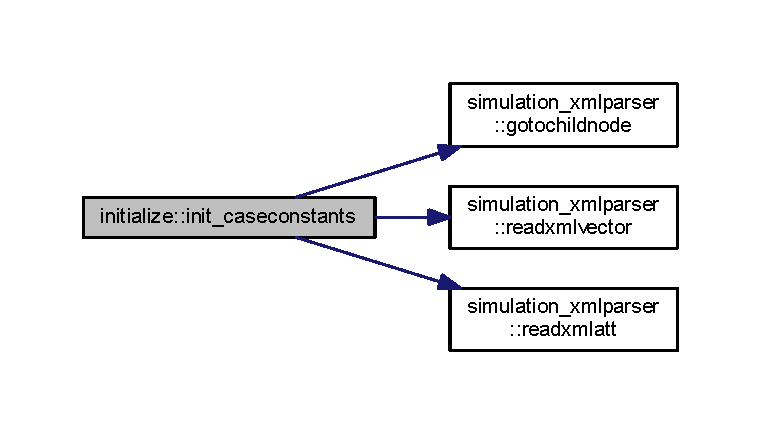
\includegraphics[width=350pt]{namespaceinitialize_a4c982b312ab10bf112dd3d2bc314569e_cgraph}
\end{center}
\end{figure}
Here is the caller graph for this function\+:
\nopagebreak
\begin{figure}[H]
\begin{center}
\leavevmode
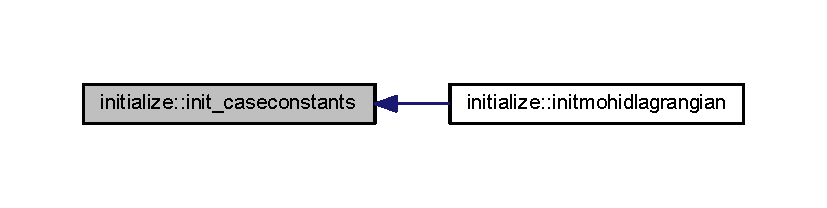
\includegraphics[width=350pt]{namespaceinitialize_a4c982b312ab10bf112dd3d2bc314569e_icgraph}
\end{center}
\end{figure}
\mbox{\Hypertarget{namespaceinitialize_a7a54dc126f448bea2b566339a449f85c}\label{namespaceinitialize_a7a54dc126f448bea2b566339a449f85c}} 
\index{initialize@{initialize}!init\+\_\+parameters@{init\+\_\+parameters}}
\index{init\+\_\+parameters@{init\+\_\+parameters}!initialize@{initialize}}
\subsubsection{\texorpdfstring{init\+\_\+parameters()}{init\_parameters()}}
{\footnotesize\ttfamily subroutine initialize\+::init\+\_\+parameters (\begin{DoxyParamCaption}\item[{type(node), intent(in), pointer}]{execution\+\_\+node }\end{DoxyParamCaption})\hspace{0.3cm}{\ttfamily [private]}}



Birjukovs Canelas -\/ M\+A\+R\+E\+T\+EC 

Private parameter parser routine. Builds the simulation parametric space from the input xml case file. 
\begin{DoxyParams}[1]{Parameters}
\mbox{\tt in}  & {\em parsedxml} & \\
\hline
\end{DoxyParams}
Here is the call graph for this function\+:
\nopagebreak
\begin{figure}[H]
\begin{center}
\leavevmode
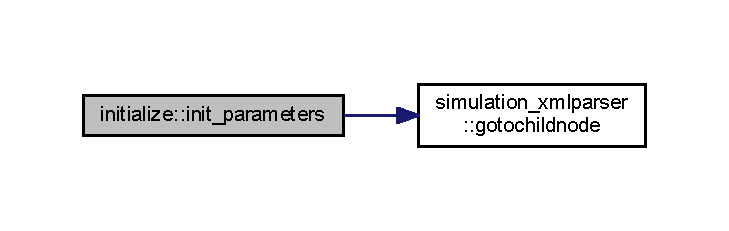
\includegraphics[width=350pt]{namespaceinitialize_a7a54dc126f448bea2b566339a449f85c_cgraph}
\end{center}
\end{figure}
Here is the caller graph for this function\+:
\nopagebreak
\begin{figure}[H]
\begin{center}
\leavevmode
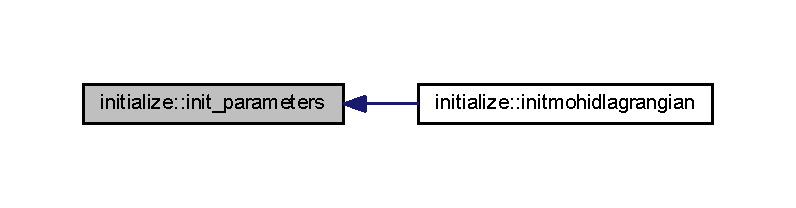
\includegraphics[width=350pt]{namespaceinitialize_a7a54dc126f448bea2b566339a449f85c_icgraph}
\end{center}
\end{figure}
\mbox{\Hypertarget{namespaceinitialize_a4640ad15e29b88467ec842f274f64b62}\label{namespaceinitialize_a4640ad15e29b88467ec842f274f64b62}} 
\index{initialize@{initialize}!init\+\_\+properties@{init\+\_\+properties}}
\index{init\+\_\+properties@{init\+\_\+properties}!initialize@{initialize}}
\subsubsection{\texorpdfstring{init\+\_\+properties()}{init\_properties()}}
{\footnotesize\ttfamily subroutine initialize\+::init\+\_\+properties (\begin{DoxyParamCaption}\item[{type(node), intent(in), pointer}]{case\+\_\+node }\end{DoxyParamCaption})\hspace{0.3cm}{\ttfamily [private]}}



Birjukovs Canelas -\/ M\+A\+R\+E\+T\+EC 

Private property xml parser routine. Reads the properties tab from the xml file and links these to the corresponding source 
\begin{DoxyParams}[1]{Parameters}
\mbox{\tt in}  & {\em parsedxml} & \\
\hline
\end{DoxyParams}
Here is the call graph for this function\+:
\nopagebreak
\begin{figure}[H]
\begin{center}
\leavevmode
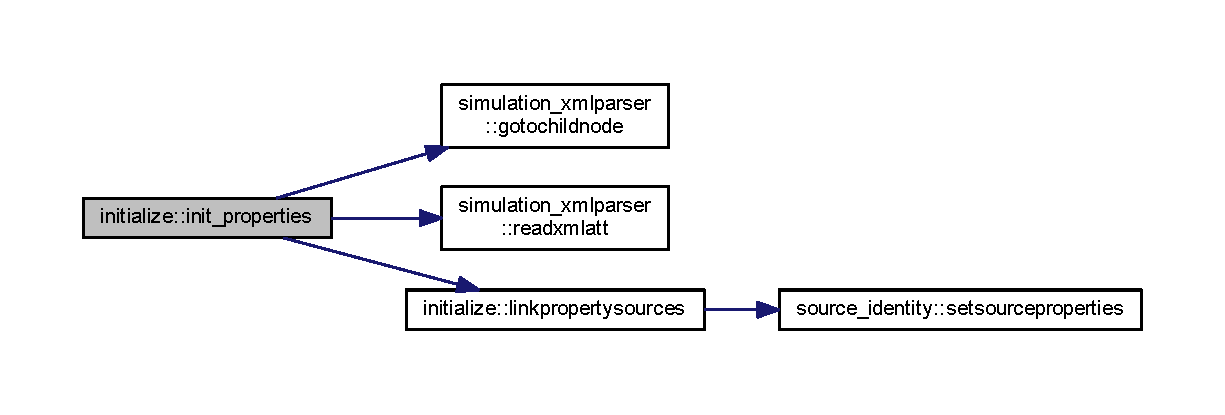
\includegraphics[width=350pt]{namespaceinitialize_a4640ad15e29b88467ec842f274f64b62_cgraph}
\end{center}
\end{figure}
Here is the caller graph for this function\+:
\nopagebreak
\begin{figure}[H]
\begin{center}
\leavevmode
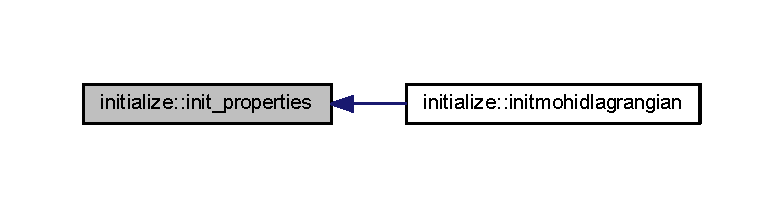
\includegraphics[width=350pt]{namespaceinitialize_a4640ad15e29b88467ec842f274f64b62_icgraph}
\end{center}
\end{figure}
\mbox{\Hypertarget{namespaceinitialize_adb972e92da4789506ee6b62b702df2b3}\label{namespaceinitialize_adb972e92da4789506ee6b62b702df2b3}} 
\index{initialize@{initialize}!init\+\_\+simdefs@{init\+\_\+simdefs}}
\index{init\+\_\+simdefs@{init\+\_\+simdefs}!initialize@{initialize}}
\subsubsection{\texorpdfstring{init\+\_\+simdefs()}{init\_simdefs()}}
{\footnotesize\ttfamily subroutine initialize\+::init\+\_\+simdefs (\begin{DoxyParamCaption}\item[{type(node), intent(in), pointer}]{case\+\_\+node }\end{DoxyParamCaption})\hspace{0.3cm}{\ttfamily [private]}}



Birjukovs Canelas -\/ M\+A\+R\+E\+T\+EC 

Private simulation definitions parser routine. Builds the simulation geometric space from the input xml case file. 
\begin{DoxyParams}[1]{Parameters}
\mbox{\tt in}  & {\em parsedxml} & \\
\hline
\end{DoxyParams}
Here is the call graph for this function\+:
\nopagebreak
\begin{figure}[H]
\begin{center}
\leavevmode
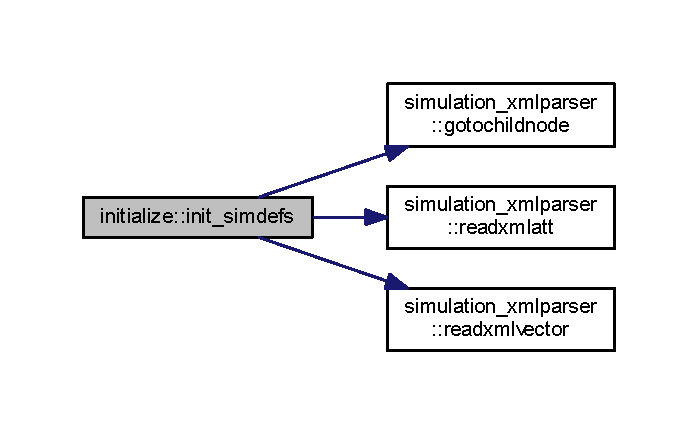
\includegraphics[width=335pt]{namespaceinitialize_adb972e92da4789506ee6b62b702df2b3_cgraph}
\end{center}
\end{figure}
Here is the caller graph for this function\+:
\nopagebreak
\begin{figure}[H]
\begin{center}
\leavevmode
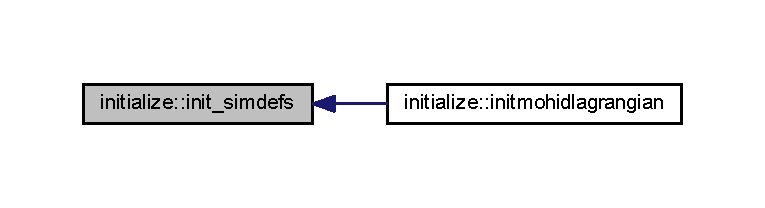
\includegraphics[width=350pt]{namespaceinitialize_adb972e92da4789506ee6b62b702df2b3_icgraph}
\end{center}
\end{figure}
\mbox{\Hypertarget{namespaceinitialize_a9ed75476e5dd07928aed3442281930be}\label{namespaceinitialize_a9ed75476e5dd07928aed3442281930be}} 
\index{initialize@{initialize}!init\+\_\+sources@{init\+\_\+sources}}
\index{init\+\_\+sources@{init\+\_\+sources}!initialize@{initialize}}
\subsubsection{\texorpdfstring{init\+\_\+sources()}{init\_sources()}}
{\footnotesize\ttfamily subroutine initialize\+::init\+\_\+sources (\begin{DoxyParamCaption}\item[{type(node), intent(in), pointer}]{case\+\_\+node }\end{DoxyParamCaption})\hspace{0.3cm}{\ttfamily [private]}}



Birjukovs Canelas -\/ M\+A\+R\+E\+T\+EC 

Private source definitions parser routine. Builds the tracer sources from the input xml case file. 
\begin{DoxyParams}[1]{Parameters}
\mbox{\tt in}  & {\em parsedxml} & \\
\hline
\end{DoxyParams}
Here is the call graph for this function\+:
\nopagebreak
\begin{figure}[H]
\begin{center}
\leavevmode
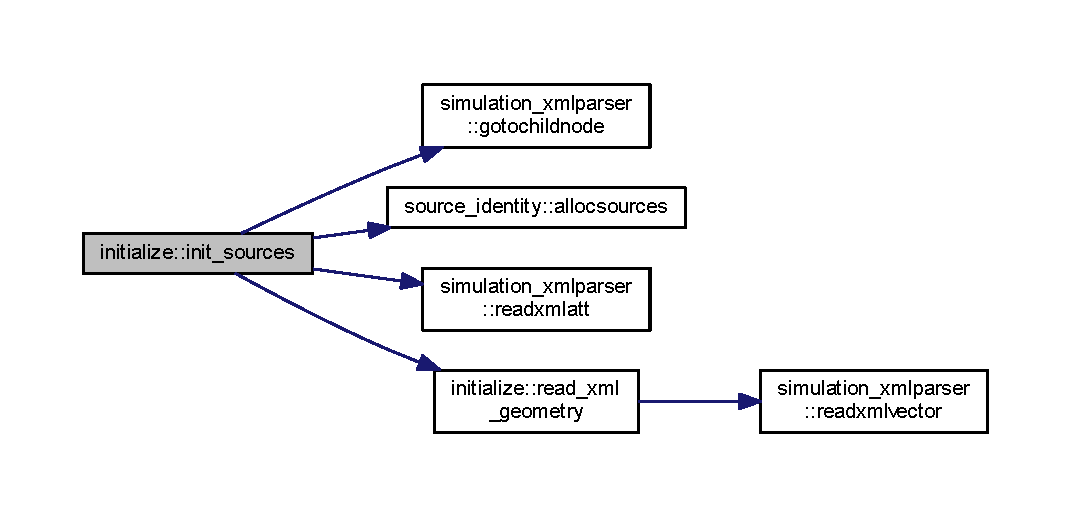
\includegraphics[width=350pt]{namespaceinitialize_a9ed75476e5dd07928aed3442281930be_cgraph}
\end{center}
\end{figure}
Here is the caller graph for this function\+:
\nopagebreak
\begin{figure}[H]
\begin{center}
\leavevmode
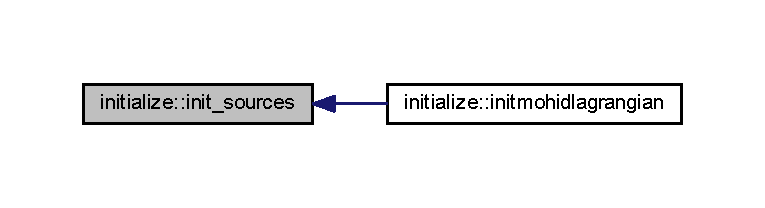
\includegraphics[width=350pt]{namespaceinitialize_a9ed75476e5dd07928aed3442281930be_icgraph}
\end{center}
\end{figure}
\mbox{\Hypertarget{namespaceinitialize_a45b7ca20c45cf272acbc391950cbb804}\label{namespaceinitialize_a45b7ca20c45cf272acbc391950cbb804}} 
\index{initialize@{initialize}!initmohidlagrangian@{initmohidlagrangian}}
\index{initmohidlagrangian@{initmohidlagrangian}!initialize@{initialize}}
\subsubsection{\texorpdfstring{initmohidlagrangian()}{initmohidlagrangian()}}
{\footnotesize\ttfamily subroutine, public initialize\+::initmohidlagrangian (\begin{DoxyParamCaption}\item[{type(string), intent(in)}]{xmlfilename }\end{DoxyParamCaption})}



Birjukovs Canelas -\/ M\+A\+R\+E\+T\+EC 

Public xml parser routine. Builds the simulation space from the input xml case file. 
\begin{DoxyParams}[1]{Parameters}
\mbox{\tt in}  & {\em xmlfilename} & \\
\hline
\mbox{\tt in}  & {\em xmlfilename} & .xml file name \\
\hline
\end{DoxyParams}
Here is the call graph for this function\+:
\nopagebreak
\begin{figure}[H]
\begin{center}
\leavevmode
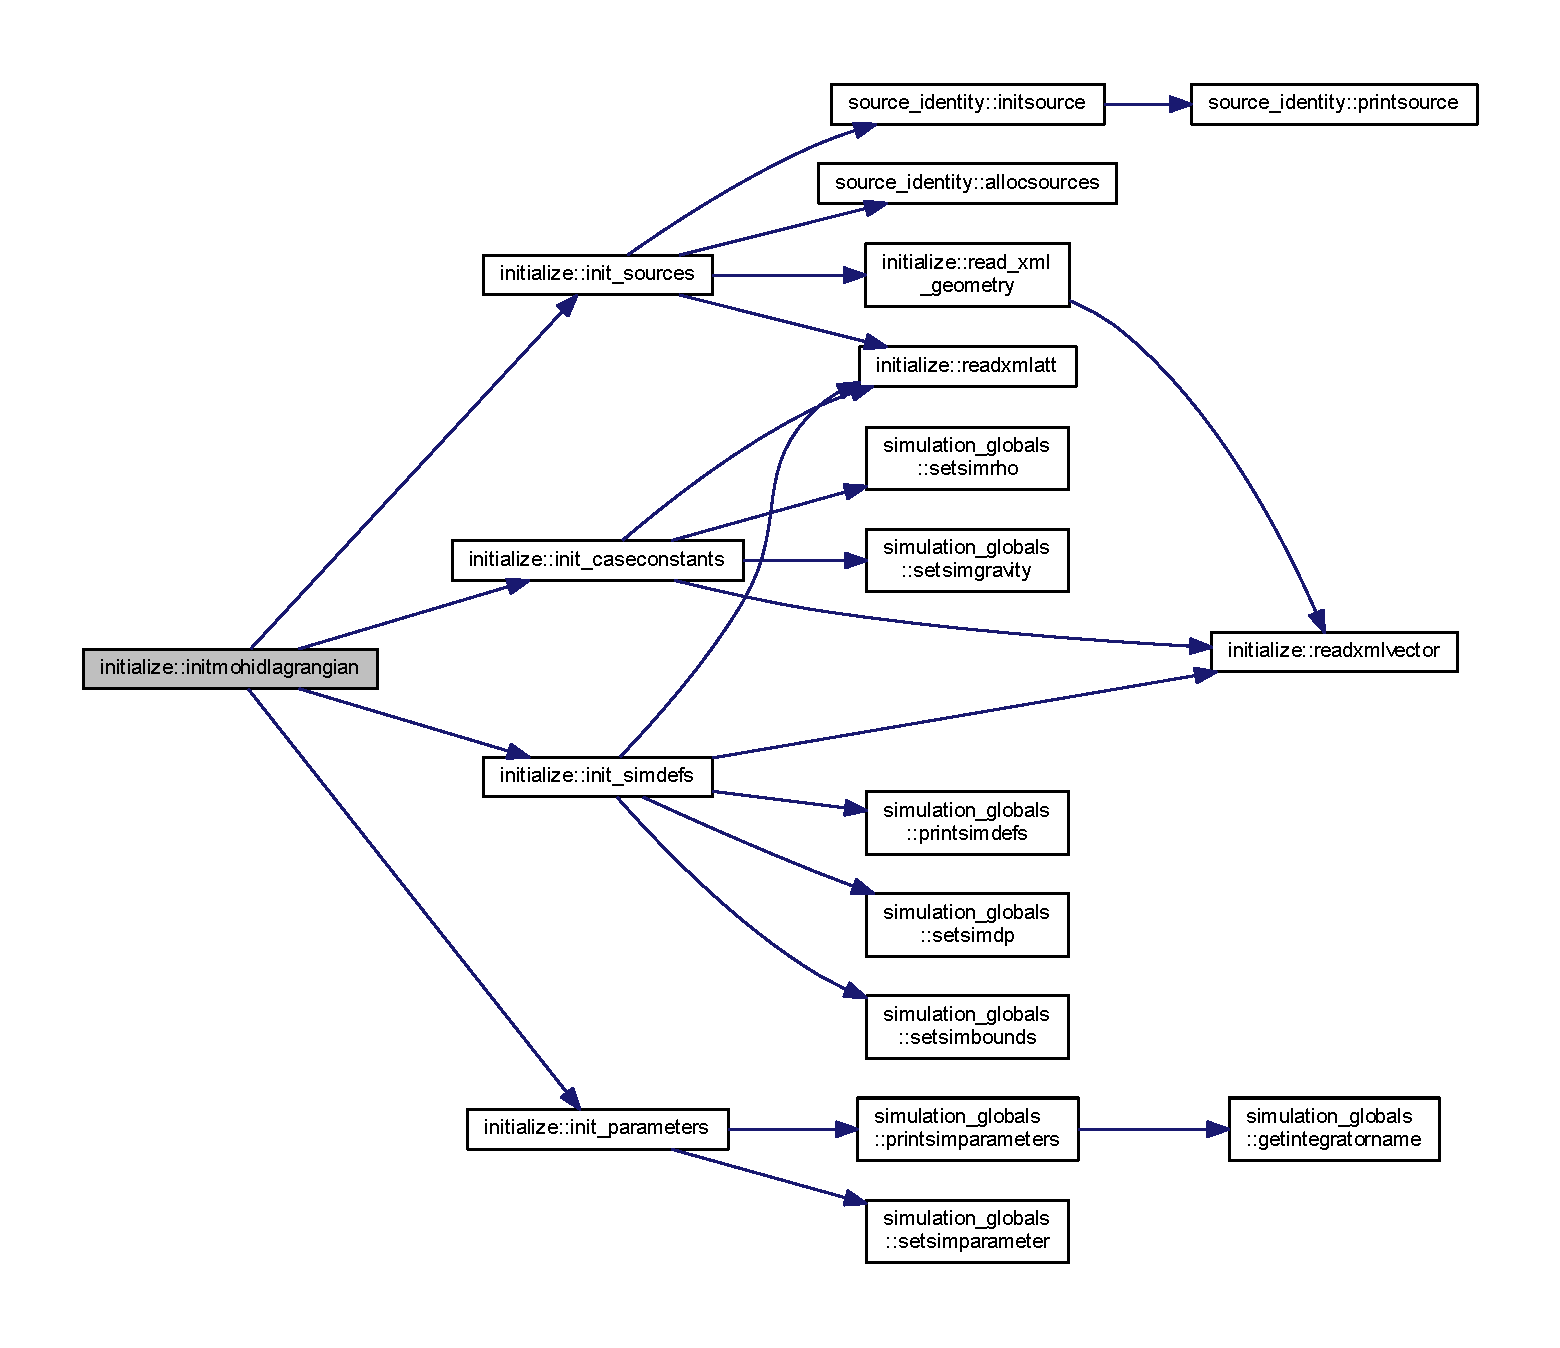
\includegraphics[width=350pt]{namespaceinitialize_a45b7ca20c45cf272acbc391950cbb804_cgraph}
\end{center}
\end{figure}
\mbox{\Hypertarget{namespaceinitialize_ab91b27efd537a161ee9ca4b2d9efde1a}\label{namespaceinitialize_ab91b27efd537a161ee9ca4b2d9efde1a}} 
\index{initialize@{initialize}!linkpropertysources@{linkpropertysources}}
\index{linkpropertysources@{linkpropertysources}!initialize@{initialize}}
\subsubsection{\texorpdfstring{linkpropertysources()}{linkpropertysources()}}
{\footnotesize\ttfamily subroutine initialize\+::linkpropertysources (\begin{DoxyParamCaption}\item[{type(node), intent(in), pointer}]{links\+Node }\end{DoxyParamCaption})\hspace{0.3cm}{\ttfamily [private]}}



Birjukovs Canelas -\/ M\+A\+R\+E\+T\+EC 

Private property xml parser routine. Reads the properties tab from the xml file and links these to the corresponding source 
\begin{DoxyParams}[1]{Parameters}
\mbox{\tt in}  & {\em parsedxml} & \\
\hline
\end{DoxyParams}
Here is the call graph for this function\+:
\nopagebreak
\begin{figure}[H]
\begin{center}
\leavevmode
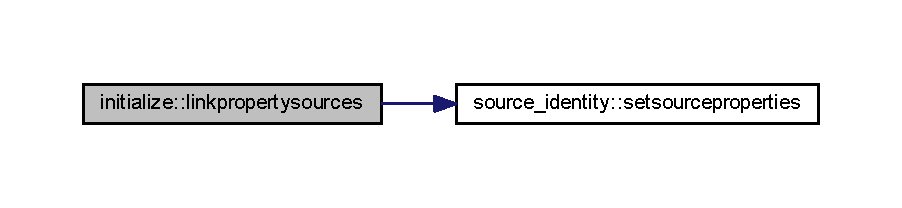
\includegraphics[width=350pt]{namespaceinitialize_ab91b27efd537a161ee9ca4b2d9efde1a_cgraph}
\end{center}
\end{figure}
Here is the caller graph for this function\+:
\nopagebreak
\begin{figure}[H]
\begin{center}
\leavevmode
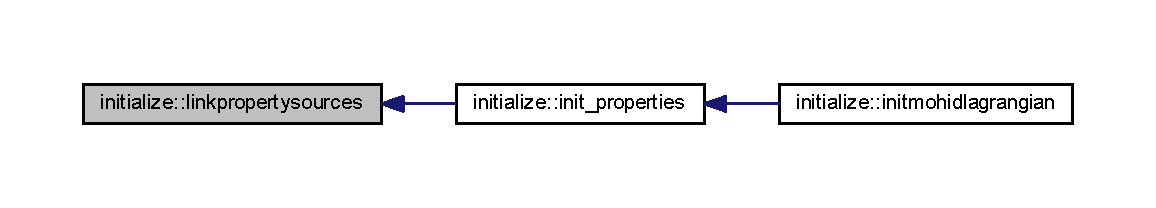
\includegraphics[width=350pt]{namespaceinitialize_ab91b27efd537a161ee9ca4b2d9efde1a_icgraph}
\end{center}
\end{figure}
\mbox{\Hypertarget{namespaceinitialize_ad36e4f602dab66c06a1f0e2474e9f0a6}\label{namespaceinitialize_ad36e4f602dab66c06a1f0e2474e9f0a6}} 
\index{initialize@{initialize}!read\+\_\+xml\+\_\+geometry@{read\+\_\+xml\+\_\+geometry}}
\index{read\+\_\+xml\+\_\+geometry@{read\+\_\+xml\+\_\+geometry}!initialize@{initialize}}
\subsubsection{\texorpdfstring{read\+\_\+xml\+\_\+geometry()}{read\_xml\_geometry()}}
{\footnotesize\ttfamily subroutine initialize\+::read\+\_\+xml\+\_\+geometry (\begin{DoxyParamCaption}\item[{type(node), intent(in), pointer}]{source,  }\item[{type(node), intent(in), pointer}]{source\+\_\+detail,  }\item[{class(\mbox{\hyperlink{structgeometry_1_1shape}{shape}}), intent(inout)}]{geometry }\end{DoxyParamCaption})\hspace{0.3cm}{\ttfamily [private]}}



Birjukovs Canelas -\/ M\+A\+R\+E\+T\+EC 

Private geometry xml parser routine. Reads a geometry from the xml depending on the geometry type of the node 
\begin{DoxyParams}[1]{Parameters}
\mbox{\tt in}  & {\em source,geometry} & \\
\hline
\mbox{\tt in}  & {\em source} & Working xml node\\
\hline
\mbox{\tt in}  & {\em source\+\_\+detail} & Working xml node details\\
\hline
\mbox{\tt in,out}  & {\em geometry} & Geometrical object to fill \\
\hline
\end{DoxyParams}
Here is the call graph for this function\+:
\nopagebreak
\begin{figure}[H]
\begin{center}
\leavevmode
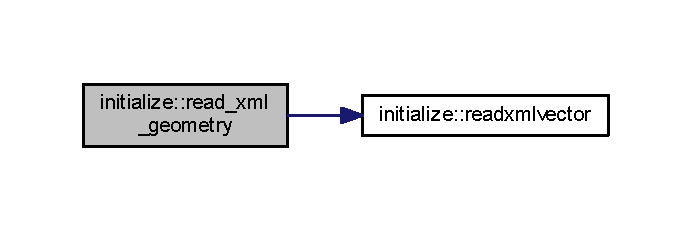
\includegraphics[width=323pt]{namespaceinitialize_ad36e4f602dab66c06a1f0e2474e9f0a6_cgraph}
\end{center}
\end{figure}
Here is the caller graph for this function\+:
\nopagebreak
\begin{figure}[H]
\begin{center}
\leavevmode
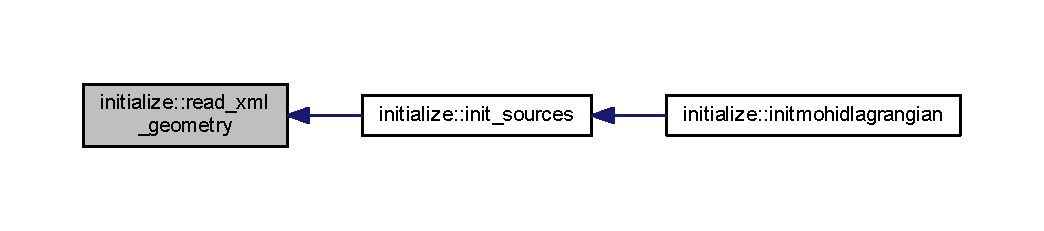
\includegraphics[width=350pt]{namespaceinitialize_ad36e4f602dab66c06a1f0e2474e9f0a6_icgraph}
\end{center}
\end{figure}

\hypertarget{namespacesimulation__globals}{}\section{simulation\+\_\+globals Module Reference}
\label{namespacesimulation__globals}\index{simulation\+\_\+globals@{simulation\+\_\+globals}}


Module to hold the simulation global parameter classes and their methods.  


\subsection*{Data Types}
\begin{DoxyCompactItemize}
\item 
type \mbox{\hyperlink{structsimulation__globals_1_1constants__t}{constants\+\_\+t}}
\begin{DoxyCompactList}\small\item\em Case Constants class. \end{DoxyCompactList}\item 
type \mbox{\hyperlink{structsimulation__globals_1_1filenames__t}{filenames\+\_\+t}}
\begin{DoxyCompactList}\small\item\em File names class. \end{DoxyCompactList}\item 
type \mbox{\hyperlink{structsimulation__globals_1_1parameters__t}{parameters\+\_\+t}}
\item 
type \mbox{\hyperlink{structsimulation__globals_1_1simdefs__t}{simdefs\+\_\+t}}
\begin{DoxyCompactList}\small\item\em Simulation definitions class. \end{DoxyCompactList}\end{DoxyCompactItemize}
\subsection*{Functions/\+Subroutines}
\begin{DoxyCompactItemize}
\item 
subroutine \mbox{\hyperlink{namespacesimulation__globals_aed3f671899558008ae9f0f009f581baf}{setparameter}} (self, parmkey, parmvalue)
\begin{DoxyCompactList}\small\item\em Birjukovs Canelas -\/ M\+A\+R\+E\+T\+EC \end{DoxyCompactList}\item 
subroutine \mbox{\hyperlink{namespacesimulation__globals_a3867df0f77dca3700c9470aea24fd048}{check}} (self)
\begin{DoxyCompactList}\small\item\em Birjukovs Canelas -\/ M\+A\+R\+E\+T\+EC \end{DoxyCompactList}\item 
subroutine \mbox{\hyperlink{namespacesimulation__globals_a0b17b2f2e9e7dbbad7c9d735217c1ee1}{printsimparameters}} (self)
\begin{DoxyCompactList}\small\item\em Birjukovs Canelas -\/ M\+A\+R\+E\+T\+EC \end{DoxyCompactList}\item 
subroutine \mbox{\hyperlink{namespacesimulation__globals_a2c6bf88542c503d1da58280ab3dcf772}{getintegratorname}} (name, code)
\begin{DoxyCompactList}\small\item\em Birjukovs Canelas -\/ M\+A\+R\+E\+T\+EC \end{DoxyCompactList}\item 
subroutine \mbox{\hyperlink{namespacesimulation__globals_ac655f60155581a71b312f3c1a8c87db2}{setgravity}} (self, grav)
\begin{DoxyCompactList}\small\item\em Birjukovs Canelas -\/ M\+A\+R\+E\+T\+EC \end{DoxyCompactList}\item 
subroutine \mbox{\hyperlink{namespacesimulation__globals_acfdc640757f0275bccb1d8de7bd7dc92}{setrho}} (self, read\+\_\+rho)
\begin{DoxyCompactList}\small\item\em Birjukovs Canelas -\/ M\+A\+R\+E\+T\+EC \end{DoxyCompactList}\item 
subroutine \mbox{\hyperlink{namespacesimulation__globals_a9a8e88c06937b7cf6be9d9bf30f54ba9}{setdp}} (self, read\+\_\+dp)
\begin{DoxyCompactList}\small\item\em Birjukovs Canelas -\/ M\+A\+R\+E\+T\+EC \end{DoxyCompactList}\item 
subroutine \mbox{\hyperlink{namespacesimulation__globals_a3ef0462db5a60ac79304cabd2fdd914d}{setdt}} (self, read\+\_\+dt)
\begin{DoxyCompactList}\small\item\em Birjukovs Canelas -\/ M\+A\+R\+E\+T\+EC \end{DoxyCompactList}\item 
subroutine \mbox{\hyperlink{namespacesimulation__globals_a1fc4653684d73efecdbd140b6cafe541}{setboundingbox}} (self, point\+\_\+, coords)
\begin{DoxyCompactList}\small\item\em Birjukovs Canelas -\/ M\+A\+R\+E\+T\+EC \end{DoxyCompactList}\item 
subroutine \mbox{\hyperlink{namespacesimulation__globals_ad90d6959da1d43e2cd1febff82187ed5}{printsimdefs}} (self)
\begin{DoxyCompactList}\small\item\em Birjukovs Canelas -\/ M\+A\+R\+E\+T\+EC \end{DoxyCompactList}\end{DoxyCompactItemize}
\subsection*{Variables}
\begin{DoxyCompactItemize}
\item 
real(prec\+\_\+time), public \mbox{\hyperlink{namespacesimulation__globals_a10daac198c63b06f99ec0c01b614a352}{simtime}}
\item 
type(\mbox{\hyperlink{structsimulation__globals_1_1parameters__t}{parameters\+\_\+t}}), public \mbox{\hyperlink{namespacesimulation__globals_ac23e87cbb2256792d683ab1bf5dc5e21}{parameters}}
\item 
type(\mbox{\hyperlink{structsimulation__globals_1_1simdefs__t}{simdefs\+\_\+t}}), public \mbox{\hyperlink{namespacesimulation__globals_ae851f977b442737307cd4bb76f2f68be}{simdefs}}
\item 
type(\mbox{\hyperlink{structsimulation__globals_1_1constants__t}{constants\+\_\+t}}), public \mbox{\hyperlink{namespacesimulation__globals_aa3e1a54abbb08d2c09978a3509ec4303}{constants}}
\item 
type(\mbox{\hyperlink{structsimulation__globals_1_1filenames__t}{filenames\+\_\+t}}), public \mbox{\hyperlink{namespacesimulation__globals_ada5ae97821ffcb77674c3470431101e3}{filenames}}
\end{DoxyCompactItemize}


\subsection{Detailed Description}
Module to hold the simulation global parameter classes and their methods. 

\begin{DoxyAuthor}{Author}
Ricardo Birjukovs Canelas 
\end{DoxyAuthor}


\subsection{Function/\+Subroutine Documentation}
\mbox{\Hypertarget{namespacesimulation__globals_a3867df0f77dca3700c9470aea24fd048}\label{namespacesimulation__globals_a3867df0f77dca3700c9470aea24fd048}} 
\index{simulation\+\_\+globals@{simulation\+\_\+globals}!check@{check}}
\index{check@{check}!simulation\+\_\+globals@{simulation\+\_\+globals}}
\subsubsection{\texorpdfstring{check()}{check()}}
{\footnotesize\ttfamily subroutine simulation\+\_\+globals\+::check (\begin{DoxyParamCaption}\item[{class(\mbox{\hyperlink{structsimulation__globals_1_1parameters__t}{parameters\+\_\+t}}), intent(inout)}]{self }\end{DoxyParamCaption})\hspace{0.3cm}{\ttfamily [private]}}



Birjukovs Canelas -\/ M\+A\+R\+E\+T\+EC 

Private parameter checking method. Checks if mandatory parameters were set Here is the call graph for this function\+:
\nopagebreak
\begin{figure}[H]
\begin{center}
\leavevmode
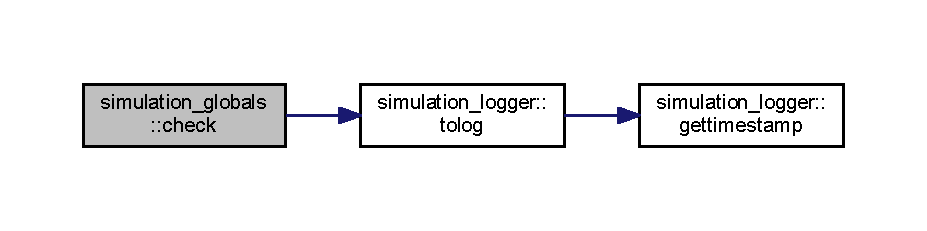
\includegraphics[width=350pt]{namespacesimulation__globals_a3867df0f77dca3700c9470aea24fd048_cgraph}
\end{center}
\end{figure}
\mbox{\Hypertarget{namespacesimulation__globals_a2c6bf88542c503d1da58280ab3dcf772}\label{namespacesimulation__globals_a2c6bf88542c503d1da58280ab3dcf772}} 
\index{simulation\+\_\+globals@{simulation\+\_\+globals}!getintegratorname@{getintegratorname}}
\index{getintegratorname@{getintegratorname}!simulation\+\_\+globals@{simulation\+\_\+globals}}
\subsubsection{\texorpdfstring{getintegratorname()}{getintegratorname()}}
{\footnotesize\ttfamily subroutine simulation\+\_\+globals\+::getintegratorname (\begin{DoxyParamCaption}\item[{type(string), intent(inout)}]{name,  }\item[{integer, intent(in)}]{code }\end{DoxyParamCaption})\hspace{0.3cm}{\ttfamily [private]}}



Birjukovs Canelas -\/ M\+A\+R\+E\+T\+EC 

private routine to get integrator scheme name Here is the caller graph for this function\+:
\nopagebreak
\begin{figure}[H]
\begin{center}
\leavevmode
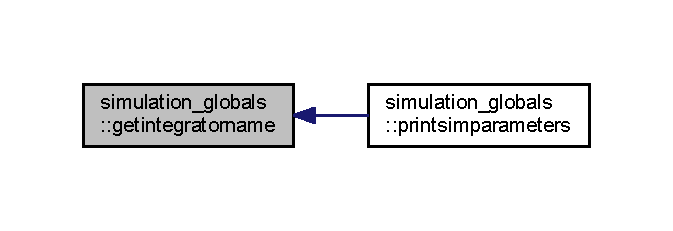
\includegraphics[width=323pt]{namespacesimulation__globals_a2c6bf88542c503d1da58280ab3dcf772_icgraph}
\end{center}
\end{figure}
\mbox{\Hypertarget{namespacesimulation__globals_ad90d6959da1d43e2cd1febff82187ed5}\label{namespacesimulation__globals_ad90d6959da1d43e2cd1febff82187ed5}} 
\index{simulation\+\_\+globals@{simulation\+\_\+globals}!printsimdefs@{printsimdefs}}
\index{printsimdefs@{printsimdefs}!simulation\+\_\+globals@{simulation\+\_\+globals}}
\subsubsection{\texorpdfstring{printsimdefs()}{printsimdefs()}}
{\footnotesize\ttfamily subroutine simulation\+\_\+globals\+::printsimdefs (\begin{DoxyParamCaption}\item[{class(\mbox{\hyperlink{structsimulation__globals_1_1simdefs__t}{simdefs\+\_\+t}}), intent(in)}]{self }\end{DoxyParamCaption})\hspace{0.3cm}{\ttfamily [private]}}



Birjukovs Canelas -\/ M\+A\+R\+E\+T\+EC 

Public simulation definitions printing routine. Here is the call graph for this function\+:
\nopagebreak
\begin{figure}[H]
\begin{center}
\leavevmode
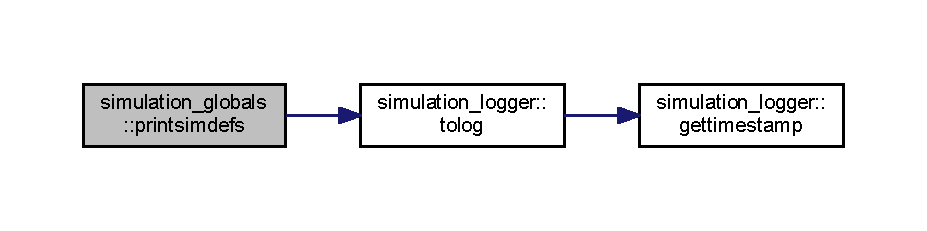
\includegraphics[width=350pt]{namespacesimulation__globals_ad90d6959da1d43e2cd1febff82187ed5_cgraph}
\end{center}
\end{figure}
\mbox{\Hypertarget{namespacesimulation__globals_a0b17b2f2e9e7dbbad7c9d735217c1ee1}\label{namespacesimulation__globals_a0b17b2f2e9e7dbbad7c9d735217c1ee1}} 
\index{simulation\+\_\+globals@{simulation\+\_\+globals}!printsimparameters@{printsimparameters}}
\index{printsimparameters@{printsimparameters}!simulation\+\_\+globals@{simulation\+\_\+globals}}
\subsubsection{\texorpdfstring{printsimparameters()}{printsimparameters()}}
{\footnotesize\ttfamily subroutine simulation\+\_\+globals\+::printsimparameters (\begin{DoxyParamCaption}\item[{class(\mbox{\hyperlink{structsimulation__globals_1_1parameters__t}{parameters\+\_\+t}}), intent(inout)}]{self }\end{DoxyParamCaption})\hspace{0.3cm}{\ttfamily [private]}}



Birjukovs Canelas -\/ M\+A\+R\+E\+T\+EC 

Private parameter printing method. Here is the call graph for this function\+:
\nopagebreak
\begin{figure}[H]
\begin{center}
\leavevmode
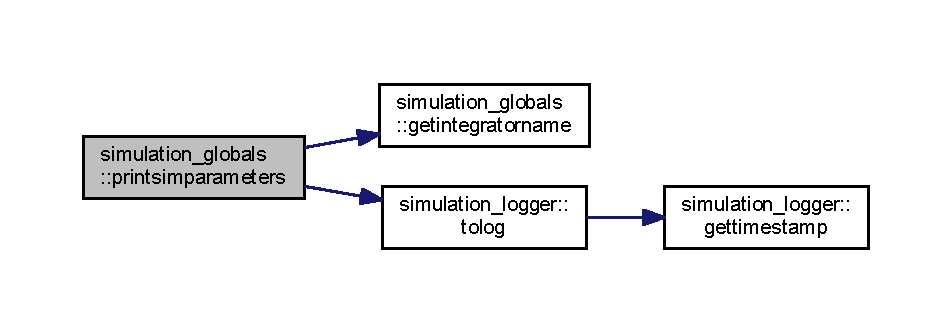
\includegraphics[width=350pt]{namespacesimulation__globals_a0b17b2f2e9e7dbbad7c9d735217c1ee1_cgraph}
\end{center}
\end{figure}
\mbox{\Hypertarget{namespacesimulation__globals_a1fc4653684d73efecdbd140b6cafe541}\label{namespacesimulation__globals_a1fc4653684d73efecdbd140b6cafe541}} 
\index{simulation\+\_\+globals@{simulation\+\_\+globals}!setboundingbox@{setboundingbox}}
\index{setboundingbox@{setboundingbox}!simulation\+\_\+globals@{simulation\+\_\+globals}}
\subsubsection{\texorpdfstring{setboundingbox()}{setboundingbox()}}
{\footnotesize\ttfamily subroutine simulation\+\_\+globals\+::setboundingbox (\begin{DoxyParamCaption}\item[{class(\mbox{\hyperlink{structsimulation__globals_1_1simdefs__t}{simdefs\+\_\+t}}), intent(inout)}]{self,  }\item[{type(string), intent(in)}]{point\+\_\+,  }\item[{type(vector)}]{coords }\end{DoxyParamCaption})\hspace{0.3cm}{\ttfamily [private]}}



Birjukovs Canelas -\/ M\+A\+R\+E\+T\+EC 

Private bounding box setting routine. 
\begin{DoxyParams}[1]{Parameters}
\mbox{\tt in}  & {\em point\+\_\+,coords} & \\
\hline
\end{DoxyParams}
\mbox{\Hypertarget{namespacesimulation__globals_a9a8e88c06937b7cf6be9d9bf30f54ba9}\label{namespacesimulation__globals_a9a8e88c06937b7cf6be9d9bf30f54ba9}} 
\index{simulation\+\_\+globals@{simulation\+\_\+globals}!setdp@{setdp}}
\index{setdp@{setdp}!simulation\+\_\+globals@{simulation\+\_\+globals}}
\subsubsection{\texorpdfstring{setdp()}{setdp()}}
{\footnotesize\ttfamily subroutine simulation\+\_\+globals\+::setdp (\begin{DoxyParamCaption}\item[{class(\mbox{\hyperlink{structsimulation__globals_1_1simdefs__t}{simdefs\+\_\+t}}), intent(inout)}]{self,  }\item[{type(string), intent(in)}]{read\+\_\+dp }\end{DoxyParamCaption})\hspace{0.3cm}{\ttfamily [private]}}



Birjukovs Canelas -\/ M\+A\+R\+E\+T\+EC 

Private dp setting routine. 
\begin{DoxyParams}[1]{Parameters}
\mbox{\tt in}  & {\em read\+\_\+dp} & \\
\hline
\end{DoxyParams}
Here is the call graph for this function\+:
\nopagebreak
\begin{figure}[H]
\begin{center}
\leavevmode
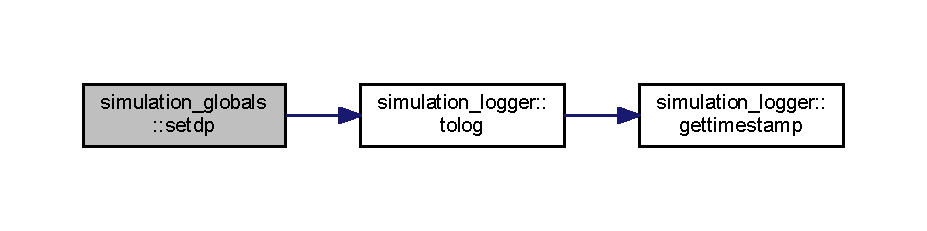
\includegraphics[width=350pt]{namespacesimulation__globals_a9a8e88c06937b7cf6be9d9bf30f54ba9_cgraph}
\end{center}
\end{figure}
\mbox{\Hypertarget{namespacesimulation__globals_a3ef0462db5a60ac79304cabd2fdd914d}\label{namespacesimulation__globals_a3ef0462db5a60ac79304cabd2fdd914d}} 
\index{simulation\+\_\+globals@{simulation\+\_\+globals}!setdt@{setdt}}
\index{setdt@{setdt}!simulation\+\_\+globals@{simulation\+\_\+globals}}
\subsubsection{\texorpdfstring{setdt()}{setdt()}}
{\footnotesize\ttfamily subroutine simulation\+\_\+globals\+::setdt (\begin{DoxyParamCaption}\item[{class(\mbox{\hyperlink{structsimulation__globals_1_1simdefs__t}{simdefs\+\_\+t}}), intent(inout)}]{self,  }\item[{type(string), intent(in)}]{read\+\_\+dt }\end{DoxyParamCaption})\hspace{0.3cm}{\ttfamily [private]}}



Birjukovs Canelas -\/ M\+A\+R\+E\+T\+EC 

Private dt setting routine. 
\begin{DoxyParams}[1]{Parameters}
\mbox{\tt in}  & {\em read\+\_\+dt} & \\
\hline
\end{DoxyParams}
Here is the call graph for this function\+:
\nopagebreak
\begin{figure}[H]
\begin{center}
\leavevmode
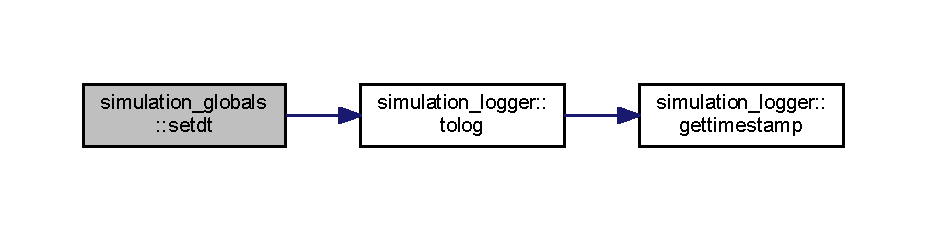
\includegraphics[width=350pt]{namespacesimulation__globals_a3ef0462db5a60ac79304cabd2fdd914d_cgraph}
\end{center}
\end{figure}
\mbox{\Hypertarget{namespacesimulation__globals_ac655f60155581a71b312f3c1a8c87db2}\label{namespacesimulation__globals_ac655f60155581a71b312f3c1a8c87db2}} 
\index{simulation\+\_\+globals@{simulation\+\_\+globals}!setgravity@{setgravity}}
\index{setgravity@{setgravity}!simulation\+\_\+globals@{simulation\+\_\+globals}}
\subsubsection{\texorpdfstring{setgravity()}{setgravity()}}
{\footnotesize\ttfamily subroutine simulation\+\_\+globals\+::setgravity (\begin{DoxyParamCaption}\item[{class(\mbox{\hyperlink{structsimulation__globals_1_1constants__t}{constants\+\_\+t}}), intent(inout)}]{self,  }\item[{type(vector)}]{grav }\end{DoxyParamCaption})\hspace{0.3cm}{\ttfamily [private]}}



Birjukovs Canelas -\/ M\+A\+R\+E\+T\+EC 

Public Gravity setting routine. 
\begin{DoxyParams}[1]{Parameters}
\mbox{\tt in}  & {\em grav} & \\
\hline
\end{DoxyParams}
\mbox{\Hypertarget{namespacesimulation__globals_aed3f671899558008ae9f0f009f581baf}\label{namespacesimulation__globals_aed3f671899558008ae9f0f009f581baf}} 
\index{simulation\+\_\+globals@{simulation\+\_\+globals}!setparameter@{setparameter}}
\index{setparameter@{setparameter}!simulation\+\_\+globals@{simulation\+\_\+globals}}
\subsubsection{\texorpdfstring{setparameter()}{setparameter()}}
{\footnotesize\ttfamily subroutine simulation\+\_\+globals\+::setparameter (\begin{DoxyParamCaption}\item[{class(\mbox{\hyperlink{structsimulation__globals_1_1parameters__t}{parameters\+\_\+t}}), intent(inout)}]{self,  }\item[{type(string), intent(in)}]{parmkey,  }\item[{type(string), intent(in)}]{parmvalue }\end{DoxyParamCaption})\hspace{0.3cm}{\ttfamily [private]}}



Birjukovs Canelas -\/ M\+A\+R\+E\+T\+EC 

Private parameter setting method. Builds the simulation parametric space from the input case file. 
\begin{DoxyParams}[1]{Parameters}
\mbox{\tt in}  & {\em parmkey,parmvalue} & \\
\hline
\end{DoxyParams}
\mbox{\Hypertarget{namespacesimulation__globals_acfdc640757f0275bccb1d8de7bd7dc92}\label{namespacesimulation__globals_acfdc640757f0275bccb1d8de7bd7dc92}} 
\index{simulation\+\_\+globals@{simulation\+\_\+globals}!setrho@{setrho}}
\index{setrho@{setrho}!simulation\+\_\+globals@{simulation\+\_\+globals}}
\subsubsection{\texorpdfstring{setrho()}{setrho()}}
{\footnotesize\ttfamily subroutine simulation\+\_\+globals\+::setrho (\begin{DoxyParamCaption}\item[{class(\mbox{\hyperlink{structsimulation__globals_1_1constants__t}{constants\+\_\+t}}), intent(inout)}]{self,  }\item[{type(string), intent(in)}]{read\+\_\+rho }\end{DoxyParamCaption})\hspace{0.3cm}{\ttfamily [private]}}



Birjukovs Canelas -\/ M\+A\+R\+E\+T\+EC 

Provate Rho\+\_\+\+Ref setting routine. 
\begin{DoxyParams}[1]{Parameters}
\mbox{\tt in}  & {\em read\+\_\+rho} & \\
\hline
\end{DoxyParams}
Here is the call graph for this function\+:
\nopagebreak
\begin{figure}[H]
\begin{center}
\leavevmode
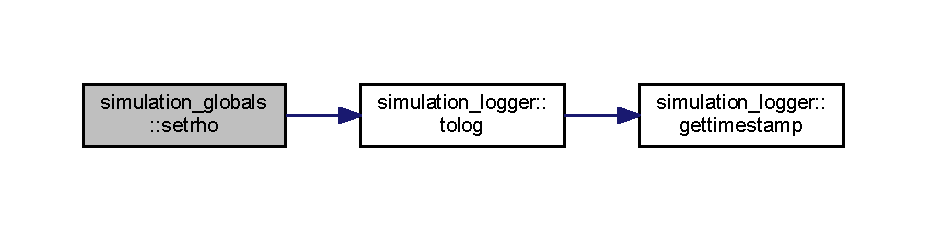
\includegraphics[width=350pt]{namespacesimulation__globals_acfdc640757f0275bccb1d8de7bd7dc92_cgraph}
\end{center}
\end{figure}


\subsection{Variable Documentation}
\mbox{\Hypertarget{namespacesimulation__globals_aa3e1a54abbb08d2c09978a3509ec4303}\label{namespacesimulation__globals_aa3e1a54abbb08d2c09978a3509ec4303}} 
\index{simulation\+\_\+globals@{simulation\+\_\+globals}!constants@{constants}}
\index{constants@{constants}!simulation\+\_\+globals@{simulation\+\_\+globals}}
\subsubsection{\texorpdfstring{constants}{constants}}
{\footnotesize\ttfamily type(\mbox{\hyperlink{structsimulation__globals_1_1constants__t}{constants\+\_\+t}}), public simulation\+\_\+globals\+::constants}

\mbox{\Hypertarget{namespacesimulation__globals_ada5ae97821ffcb77674c3470431101e3}\label{namespacesimulation__globals_ada5ae97821ffcb77674c3470431101e3}} 
\index{simulation\+\_\+globals@{simulation\+\_\+globals}!filenames@{filenames}}
\index{filenames@{filenames}!simulation\+\_\+globals@{simulation\+\_\+globals}}
\subsubsection{\texorpdfstring{filenames}{filenames}}
{\footnotesize\ttfamily type(\mbox{\hyperlink{structsimulation__globals_1_1filenames__t}{filenames\+\_\+t}}), public simulation\+\_\+globals\+::filenames}

\mbox{\Hypertarget{namespacesimulation__globals_ac23e87cbb2256792d683ab1bf5dc5e21}\label{namespacesimulation__globals_ac23e87cbb2256792d683ab1bf5dc5e21}} 
\index{simulation\+\_\+globals@{simulation\+\_\+globals}!parameters@{parameters}}
\index{parameters@{parameters}!simulation\+\_\+globals@{simulation\+\_\+globals}}
\subsubsection{\texorpdfstring{parameters}{parameters}}
{\footnotesize\ttfamily type(\mbox{\hyperlink{structsimulation__globals_1_1parameters__t}{parameters\+\_\+t}}), public simulation\+\_\+globals\+::parameters}

\mbox{\Hypertarget{namespacesimulation__globals_ae851f977b442737307cd4bb76f2f68be}\label{namespacesimulation__globals_ae851f977b442737307cd4bb76f2f68be}} 
\index{simulation\+\_\+globals@{simulation\+\_\+globals}!simdefs@{simdefs}}
\index{simdefs@{simdefs}!simulation\+\_\+globals@{simulation\+\_\+globals}}
\subsubsection{\texorpdfstring{simdefs}{simdefs}}
{\footnotesize\ttfamily type(\mbox{\hyperlink{structsimulation__globals_1_1simdefs__t}{simdefs\+\_\+t}}), public simulation\+\_\+globals\+::simdefs}

\mbox{\Hypertarget{namespacesimulation__globals_a10daac198c63b06f99ec0c01b614a352}\label{namespacesimulation__globals_a10daac198c63b06f99ec0c01b614a352}} 
\index{simulation\+\_\+globals@{simulation\+\_\+globals}!simtime@{simtime}}
\index{simtime@{simtime}!simulation\+\_\+globals@{simulation\+\_\+globals}}
\subsubsection{\texorpdfstring{simtime}{simtime}}
{\footnotesize\ttfamily real(prec\+\_\+time), public simulation\+\_\+globals\+::simtime}


\hypertarget{namespacesimulation__precision}{}\section{simulation\+\_\+precision Module Reference}
\label{namespacesimulation__precision}\index{simulation\+\_\+precision@{simulation\+\_\+precision}}


Module to control the precision of the variables trough the project.  


\subsection*{Variables}
\begin{DoxyCompactItemize}
\item 
integer, parameter \hyperlink{namespacesimulation__precision_a3657003647318cfe37c797ab37448a2e}{sp} = kind(1.\+\_\+\+R4P)
\begin{DoxyCompactList}\small\item\em Simple precision definition switch. \end{DoxyCompactList}\item 
integer, parameter \hyperlink{namespacesimulation__precision_af01fc62f503e0ff9a95c9ee2960c9a7f}{dp} = kind(1.\+\_\+\+R8P)
\begin{DoxyCompactList}\small\item\em Double precision definition switch. \end{DoxyCompactList}\item 
integer, parameter, public \hyperlink{namespacesimulation__precision_a6d3bcd3b4ff2cfb92ec9fe36ecad405b}{prec} = \hyperlink{namespacesimulation__precision_a3657003647318cfe37c797ab37448a2e}{sp}
\item 
integer, parameter, public \hyperlink{namespacesimulation__precision_a09a1db15abeed81ff2f54b363128ffed}{prec\+\_\+time} = \hyperlink{namespacesimulation__precision_a3657003647318cfe37c797ab37448a2e}{sp}
\item 
integer, parameter, public \hyperlink{namespacesimulation__precision_a049e8de4fad9c285d2cc71e8982e2971}{prec\+\_\+wrt} = \hyperlink{namespacesimulation__precision_a3657003647318cfe37c797ab37448a2e}{sp}
\item 
real(\hyperlink{namespacesimulation__precision_a6d3bcd3b4ff2cfb92ec9fe36ecad405b}{prec}), parameter, public \hyperlink{namespacesimulation__precision_a5983f631bbe7a6e5d43d2a458db81460}{missing\+\_\+value\+\_\+default} = -\/9999.\+0\+\_\+dp
\item 
real(\hyperlink{namespacesimulation__precision_a6d3bcd3b4ff2cfb92ec9fe36ecad405b}{prec}), parameter, public \hyperlink{namespacesimulation__precision_a4416a112b4fc53848f9f18fe5e9003db}{mv} = M\+I\+S\+S\+I\+N\+G\+\_\+\+V\+A\+L\+U\+E\+\_\+\+D\+E\+F\+A\+U\+LT
\item 
real(\hyperlink{namespacesimulation__precision_a6d3bcd3b4ff2cfb92ec9fe36ecad405b}{prec}), parameter, public \hyperlink{namespacesimulation__precision_ae23a853ee1499839ea702b3c01e443fc}{mv\+\_\+int} = int(M\+I\+S\+S\+I\+N\+G\+\_\+\+V\+A\+L\+U\+E\+\_\+\+D\+E\+F\+A\+U\+LT)
\item 
real(\hyperlink{namespacesimulation__precision_a6d3bcd3b4ff2cfb92ec9fe36ecad405b}{prec}), parameter, public \hyperlink{namespacesimulation__precision_acb6a32a47c43de36b53bb8033aa2738e}{err\+\_\+dist} = 1\+E8\+\_\+dp
\item 
integer, parameter, public \hyperlink{namespacesimulation__precision_a531d4e8c47b468cf4212393a5b84c7c8}{err\+\_\+ind} = -\/1
\end{DoxyCompactItemize}


\subsection{Detailed Description}
Module to control the precision of the variables trough the project. 

\begin{DoxyAuthor}{Author}
Ricardo Birjukovs Canelas 
\end{DoxyAuthor}


\subsection{Variable Documentation}
\mbox{\Hypertarget{namespacesimulation__precision_af01fc62f503e0ff9a95c9ee2960c9a7f}\label{namespacesimulation__precision_af01fc62f503e0ff9a95c9ee2960c9a7f}} 
\index{simulation\+\_\+precision@{simulation\+\_\+precision}!dp@{dp}}
\index{dp@{dp}!simulation\+\_\+precision@{simulation\+\_\+precision}}
\subsubsection{\texorpdfstring{dp}{dp}}
{\footnotesize\ttfamily integer, parameter simulation\+\_\+precision\+::dp = kind(1.\+\_\+\+R8P)\hspace{0.3cm}{\ttfamily [private]}}



Double precision definition switch. 

\mbox{\Hypertarget{namespacesimulation__precision_acb6a32a47c43de36b53bb8033aa2738e}\label{namespacesimulation__precision_acb6a32a47c43de36b53bb8033aa2738e}} 
\index{simulation\+\_\+precision@{simulation\+\_\+precision}!err\+\_\+dist@{err\+\_\+dist}}
\index{err\+\_\+dist@{err\+\_\+dist}!simulation\+\_\+precision@{simulation\+\_\+precision}}
\subsubsection{\texorpdfstring{err\+\_\+dist}{err\_dist}}
{\footnotesize\ttfamily real(\hyperlink{namespacesimulation__precision_a6d3bcd3b4ff2cfb92ec9fe36ecad405b}{prec}), parameter, public simulation\+\_\+precision\+::err\+\_\+dist = 1\+E8\+\_\+dp}

\mbox{\Hypertarget{namespacesimulation__precision_a531d4e8c47b468cf4212393a5b84c7c8}\label{namespacesimulation__precision_a531d4e8c47b468cf4212393a5b84c7c8}} 
\index{simulation\+\_\+precision@{simulation\+\_\+precision}!err\+\_\+ind@{err\+\_\+ind}}
\index{err\+\_\+ind@{err\+\_\+ind}!simulation\+\_\+precision@{simulation\+\_\+precision}}
\subsubsection{\texorpdfstring{err\+\_\+ind}{err\_ind}}
{\footnotesize\ttfamily integer, parameter, public simulation\+\_\+precision\+::err\+\_\+ind = -\/1}

\mbox{\Hypertarget{namespacesimulation__precision_a5983f631bbe7a6e5d43d2a458db81460}\label{namespacesimulation__precision_a5983f631bbe7a6e5d43d2a458db81460}} 
\index{simulation\+\_\+precision@{simulation\+\_\+precision}!missing\+\_\+value\+\_\+default@{missing\+\_\+value\+\_\+default}}
\index{missing\+\_\+value\+\_\+default@{missing\+\_\+value\+\_\+default}!simulation\+\_\+precision@{simulation\+\_\+precision}}
\subsubsection{\texorpdfstring{missing\+\_\+value\+\_\+default}{missing\_value\_default}}
{\footnotesize\ttfamily real(\hyperlink{namespacesimulation__precision_a6d3bcd3b4ff2cfb92ec9fe36ecad405b}{prec}), parameter, public simulation\+\_\+precision\+::missing\+\_\+value\+\_\+default = -\/9999.\+0\+\_\+dp}

\mbox{\Hypertarget{namespacesimulation__precision_a4416a112b4fc53848f9f18fe5e9003db}\label{namespacesimulation__precision_a4416a112b4fc53848f9f18fe5e9003db}} 
\index{simulation\+\_\+precision@{simulation\+\_\+precision}!mv@{mv}}
\index{mv@{mv}!simulation\+\_\+precision@{simulation\+\_\+precision}}
\subsubsection{\texorpdfstring{mv}{mv}}
{\footnotesize\ttfamily real(\hyperlink{namespacesimulation__precision_a6d3bcd3b4ff2cfb92ec9fe36ecad405b}{prec}), parameter, public simulation\+\_\+precision\+::mv = M\+I\+S\+S\+I\+N\+G\+\_\+\+V\+A\+L\+U\+E\+\_\+\+D\+E\+F\+A\+U\+LT}

\mbox{\Hypertarget{namespacesimulation__precision_ae23a853ee1499839ea702b3c01e443fc}\label{namespacesimulation__precision_ae23a853ee1499839ea702b3c01e443fc}} 
\index{simulation\+\_\+precision@{simulation\+\_\+precision}!mv\+\_\+int@{mv\+\_\+int}}
\index{mv\+\_\+int@{mv\+\_\+int}!simulation\+\_\+precision@{simulation\+\_\+precision}}
\subsubsection{\texorpdfstring{mv\+\_\+int}{mv\_int}}
{\footnotesize\ttfamily real(\hyperlink{namespacesimulation__precision_a6d3bcd3b4ff2cfb92ec9fe36ecad405b}{prec}), parameter, public simulation\+\_\+precision\+::mv\+\_\+int = int(M\+I\+S\+S\+I\+N\+G\+\_\+\+V\+A\+L\+U\+E\+\_\+\+D\+E\+F\+A\+U\+LT)}

\mbox{\Hypertarget{namespacesimulation__precision_a6d3bcd3b4ff2cfb92ec9fe36ecad405b}\label{namespacesimulation__precision_a6d3bcd3b4ff2cfb92ec9fe36ecad405b}} 
\index{simulation\+\_\+precision@{simulation\+\_\+precision}!prec@{prec}}
\index{prec@{prec}!simulation\+\_\+precision@{simulation\+\_\+precision}}
\subsubsection{\texorpdfstring{prec}{prec}}
{\footnotesize\ttfamily integer, parameter, public simulation\+\_\+precision\+::prec = \hyperlink{namespacesimulation__precision_a3657003647318cfe37c797ab37448a2e}{sp}}

\mbox{\Hypertarget{namespacesimulation__precision_a09a1db15abeed81ff2f54b363128ffed}\label{namespacesimulation__precision_a09a1db15abeed81ff2f54b363128ffed}} 
\index{simulation\+\_\+precision@{simulation\+\_\+precision}!prec\+\_\+time@{prec\+\_\+time}}
\index{prec\+\_\+time@{prec\+\_\+time}!simulation\+\_\+precision@{simulation\+\_\+precision}}
\subsubsection{\texorpdfstring{prec\+\_\+time}{prec\_time}}
{\footnotesize\ttfamily integer, parameter, public simulation\+\_\+precision\+::prec\+\_\+time = \hyperlink{namespacesimulation__precision_a3657003647318cfe37c797ab37448a2e}{sp}}

\mbox{\Hypertarget{namespacesimulation__precision_a049e8de4fad9c285d2cc71e8982e2971}\label{namespacesimulation__precision_a049e8de4fad9c285d2cc71e8982e2971}} 
\index{simulation\+\_\+precision@{simulation\+\_\+precision}!prec\+\_\+wrt@{prec\+\_\+wrt}}
\index{prec\+\_\+wrt@{prec\+\_\+wrt}!simulation\+\_\+precision@{simulation\+\_\+precision}}
\subsubsection{\texorpdfstring{prec\+\_\+wrt}{prec\_wrt}}
{\footnotesize\ttfamily integer, parameter, public simulation\+\_\+precision\+::prec\+\_\+wrt = \hyperlink{namespacesimulation__precision_a3657003647318cfe37c797ab37448a2e}{sp}}

\mbox{\Hypertarget{namespacesimulation__precision_a3657003647318cfe37c797ab37448a2e}\label{namespacesimulation__precision_a3657003647318cfe37c797ab37448a2e}} 
\index{simulation\+\_\+precision@{simulation\+\_\+precision}!sp@{sp}}
\index{sp@{sp}!simulation\+\_\+precision@{simulation\+\_\+precision}}
\subsubsection{\texorpdfstring{sp}{sp}}
{\footnotesize\ttfamily integer, parameter simulation\+\_\+precision\+::sp = kind(1.\+\_\+\+R4P)\hspace{0.3cm}{\ttfamily [private]}}



Simple precision definition switch. 


\hypertarget{namespacesource}{}\section{source Module Reference}
\label{namespacesource}\index{source@{source}}


Module to hold and wrap all the tracer sources respective modules. Defines a source class and related methods.  




\subsection{Detailed Description}
Module to hold and wrap all the tracer sources respective modules. Defines a source class and related methods. 

\begin{DoxyAuthor}{Author}
Ricardo Birjukovs Canelas 
\end{DoxyAuthor}

\hypertarget{namespacesource__emitter}{}\section{source\+\_\+emitter Module Reference}
\label{namespacesource__emitter}\index{source\+\_\+emitter@{source\+\_\+emitter}}


Module that defines an emitter class and related methods. This module is responsible for building a potential tracer list based on the availble sources and calling their initializers.  


\subsection*{Data Types}
\begin{DoxyCompactItemize}
\item 
type \mbox{\hyperlink{structsource__emitter_1_1emitter__t}{emitter\+\_\+t}}
\end{DoxyCompactItemize}
\subsection*{Functions/\+Subroutines}
\begin{DoxyCompactItemize}
\item 
subroutine \mbox{\hyperlink{namespacesource__emitter_a18e5a215687e0f5f13c0148be0f0c0e6}{initialize}} (self, srcs, nsrcs)
\begin{DoxyCompactList}\small\item\em Birjukovs Canelas -\/ M\+A\+R\+E\+T\+EC \end{DoxyCompactList}\item 
subroutine \mbox{\hyperlink{namespacesource__emitter_a73d054a39fc1fccfde74173a5c7f2c58}{setotalnp}} (src)
\begin{DoxyCompactList}\small\item\em Birjukovs Canelas -\/ M\+A\+R\+E\+T\+EC \end{DoxyCompactList}\end{DoxyCompactItemize}
\subsection*{Variables}
\begin{DoxyCompactItemize}
\item 
type(\mbox{\hyperlink{structsource__emitter_1_1emitter__t}{emitter\+\_\+t}}), public \mbox{\hyperlink{namespacesource__emitter_a357876a84a74e23c44e92ab8ef7dc35e}{emitter}}
\end{DoxyCompactItemize}


\subsection{Detailed Description}
Module that defines an emitter class and related methods. This module is responsible for building a potential tracer list based on the availble sources and calling their initializers. 

\begin{DoxyAuthor}{Author}
Ricardo Birjukovs Canelas 
\end{DoxyAuthor}


\subsection{Function/\+Subroutine Documentation}
\mbox{\Hypertarget{namespacesource__emitter_a18e5a215687e0f5f13c0148be0f0c0e6}\label{namespacesource__emitter_a18e5a215687e0f5f13c0148be0f0c0e6}} 
\index{source\+\_\+emitter@{source\+\_\+emitter}!initialize@{initialize}}
\index{initialize@{initialize}!source\+\_\+emitter@{source\+\_\+emitter}}
\subsubsection{\texorpdfstring{initialize()}{initialize()}}
{\footnotesize\ttfamily subroutine source\+\_\+emitter\+::initialize (\begin{DoxyParamCaption}\item[{class(\mbox{\hyperlink{structsource__emitter_1_1emitter__t}{emitter\+\_\+t}}), intent(in)}]{self,  }\item[{class(\mbox{\hyperlink{structsource__identity_1_1source__class}{source\+\_\+class}}), dimension(nsrcs), intent(inout)}]{srcs,  }\item[{integer, intent(in)}]{nsrcs }\end{DoxyParamCaption})\hspace{0.3cm}{\ttfamily [private]}}



Birjukovs Canelas -\/ M\+A\+R\+E\+T\+EC 

method that returns the total number of tracers an input source can potentially create 
\begin{DoxyParams}[1]{Parameters}
\mbox{\tt in}  & {\em self,src} & \\
\hline
\end{DoxyParams}
Here is the call graph for this function\+:\nopagebreak
\begin{figure}[H]
\begin{center}
\leavevmode
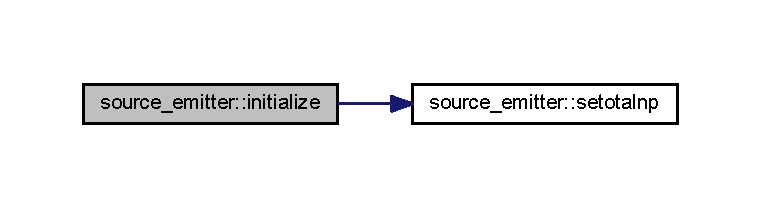
\includegraphics[width=350pt]{namespacesource__emitter_a18e5a215687e0f5f13c0148be0f0c0e6_cgraph}
\end{center}
\end{figure}
\mbox{\Hypertarget{namespacesource__emitter_a73d054a39fc1fccfde74173a5c7f2c58}\label{namespacesource__emitter_a73d054a39fc1fccfde74173a5c7f2c58}} 
\index{source\+\_\+emitter@{source\+\_\+emitter}!setotalnp@{setotalnp}}
\index{setotalnp@{setotalnp}!source\+\_\+emitter@{source\+\_\+emitter}}
\subsubsection{\texorpdfstring{setotalnp()}{setotalnp()}}
{\footnotesize\ttfamily subroutine source\+\_\+emitter\+::setotalnp (\begin{DoxyParamCaption}\item[{class(\mbox{\hyperlink{structsource__identity_1_1source__class}{source\+\_\+class}}), intent(inout)}]{src }\end{DoxyParamCaption})\hspace{0.3cm}{\ttfamily [private]}}



Birjukovs Canelas -\/ M\+A\+R\+E\+T\+EC 

private routine that returns the total number of tracers an input source will potentially create 
\begin{DoxyParams}[1]{Parameters}
\mbox{\tt in}  & {\em src} & \\
\hline
\end{DoxyParams}
${NP}_{total}^{source-i}=(T_{end}^{source-i}-T_{start}^{source-i})*{Rate}^{source-i}*{NP}_{emission}^{source-i}$ Here is the caller graph for this function\+:\nopagebreak
\begin{figure}[H]
\begin{center}
\leavevmode
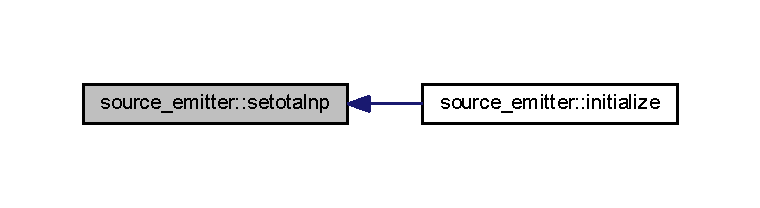
\includegraphics[width=350pt]{namespacesource__emitter_a73d054a39fc1fccfde74173a5c7f2c58_icgraph}
\end{center}
\end{figure}


\subsection{Variable Documentation}
\mbox{\Hypertarget{namespacesource__emitter_a357876a84a74e23c44e92ab8ef7dc35e}\label{namespacesource__emitter_a357876a84a74e23c44e92ab8ef7dc35e}} 
\index{source\+\_\+emitter@{source\+\_\+emitter}!emitter@{emitter}}
\index{emitter@{emitter}!source\+\_\+emitter@{source\+\_\+emitter}}
\subsubsection{\texorpdfstring{emitter}{emitter}}
{\footnotesize\ttfamily type(\mbox{\hyperlink{structsource__emitter_1_1emitter__t}{emitter\+\_\+t}}), public source\+\_\+emitter\+::emitter}


\hypertarget{namespacesource__identity}{}\section{source\+\_\+identity Module Reference}
\label{namespacesource__identity}\index{source\+\_\+identity@{source\+\_\+identity}}


Module that defines a source class and related methods.  


\subsection*{Data Types}
\begin{DoxyCompactItemize}
\item 
type \mbox{\hyperlink{structsource__identity_1_1source__class}{source\+\_\+class}}
\begin{DoxyCompactList}\small\item\em Type -\/ The source class. \end{DoxyCompactList}\item 
type \mbox{\hyperlink{structsource__identity_1_1source__par__class}{source\+\_\+par\+\_\+class}}
\item 
type \mbox{\hyperlink{structsource__identity_1_1source__state__class}{source\+\_\+state\+\_\+class}}
\begin{DoxyCompactList}\small\item\em Type -\/ state variables of a source object. \end{DoxyCompactList}\item 
type \mbox{\hyperlink{structsource__identity_1_1source__stats__class}{source\+\_\+stats\+\_\+class}}
\begin{DoxyCompactList}\small\item\em Type -\/ statistical variables of a source object. \end{DoxyCompactList}\end{DoxyCompactItemize}
\subsection*{Functions/\+Subroutines}
\begin{DoxyCompactItemize}
\item 
subroutine, public \mbox{\hyperlink{namespacesource__identity_a716b4cb4acec5756a6d4dcf20eee588e}{allocsources}} (nsources)
\begin{DoxyCompactList}\small\item\em Birjukovs Canelas -\/ M\+A\+R\+E\+T\+EC \end{DoxyCompactList}\item 
subroutine, public \mbox{\hyperlink{namespacesource__identity_a3939e59172252d0edce57e00ea41758d}{initsource}} (num, id, name, emitting\+\_\+rate, source\+\_\+geometry, geometry)
\begin{DoxyCompactList}\small\item\em Birjukovs Canelas -\/ M\+A\+R\+E\+T\+EC \end{DoxyCompactList}\item 
subroutine \mbox{\hyperlink{namespacesource__identity_ac4fc3a54de91016023a7948d261f84a5}{printsource}} (src)
\begin{DoxyCompactList}\small\item\em Birjukovs Canelas -\/ M\+A\+R\+E\+T\+EC \end{DoxyCompactList}\end{DoxyCompactItemize}
\subsection*{Variables}
\begin{DoxyCompactItemize}
\item 
type(\mbox{\hyperlink{structsource__identity_1_1source__class}{source\+\_\+class}}), dimension(\+:), allocatable, public \mbox{\hyperlink{namespacesource__identity_a5ed8006613af7461c6a2ff1cdaeb8f0f}{source}}
\end{DoxyCompactItemize}


\subsection{Detailed Description}
Module that defines a source class and related methods. 

\begin{DoxyAuthor}{Author}
Ricardo Birjukovs Canelas 
\end{DoxyAuthor}


\subsection{Function/\+Subroutine Documentation}
\mbox{\Hypertarget{namespacesource__identity_a716b4cb4acec5756a6d4dcf20eee588e}\label{namespacesource__identity_a716b4cb4acec5756a6d4dcf20eee588e}} 
\index{source\+\_\+identity@{source\+\_\+identity}!allocsources@{allocsources}}
\index{allocsources@{allocsources}!source\+\_\+identity@{source\+\_\+identity}}
\subsubsection{\texorpdfstring{allocsources()}{allocsources()}}
{\footnotesize\ttfamily subroutine, public source\+\_\+identity\+::allocsources (\begin{DoxyParamCaption}\item[{integer, intent(in)}]{nsources }\end{DoxyParamCaption})}



Birjukovs Canelas -\/ M\+A\+R\+E\+T\+EC 

source allocation routine -\/ allocates the sources objects 
\begin{DoxyParams}[1]{Parameters}
\mbox{\tt in}  & {\em nsources} & \\
\hline
\end{DoxyParams}
Here is the caller graph for this function\+:\nopagebreak
\begin{figure}[H]
\begin{center}
\leavevmode
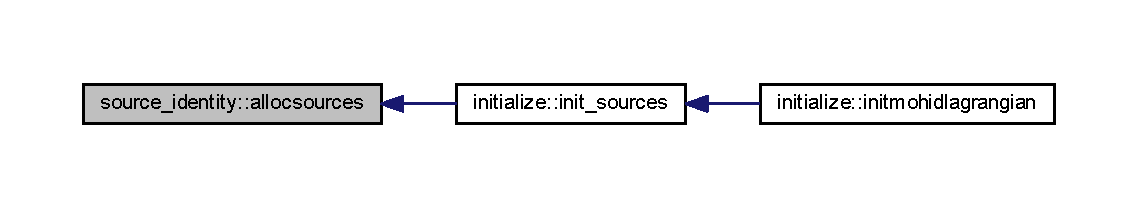
\includegraphics[width=350pt]{namespacesource__identity_a716b4cb4acec5756a6d4dcf20eee588e_icgraph}
\end{center}
\end{figure}
\mbox{\Hypertarget{namespacesource__identity_a3939e59172252d0edce57e00ea41758d}\label{namespacesource__identity_a3939e59172252d0edce57e00ea41758d}} 
\index{source\+\_\+identity@{source\+\_\+identity}!initsource@{initsource}}
\index{initsource@{initsource}!source\+\_\+identity@{source\+\_\+identity}}
\subsubsection{\texorpdfstring{initsource()}{initsource()}}
{\footnotesize\ttfamily subroutine, public source\+\_\+identity\+::initsource (\begin{DoxyParamCaption}\item[{integer, intent(in)}]{num,  }\item[{integer, intent(in)}]{id,  }\item[{type(string), intent(in)}]{name,  }\item[{real(prec), intent(in)}]{emitting\+\_\+rate,  }\item[{type(string), intent(in)}]{source\+\_\+geometry,  }\item[{class(\mbox{\hyperlink{structgeometry_1_1shape}{shape}}), intent(in)}]{geometry }\end{DoxyParamCaption})}



Birjukovs Canelas -\/ M\+A\+R\+E\+T\+EC 

source inititialization routine -\/ Generates a source and initializes its variables 
\begin{DoxyParams}[1]{Parameters}
\mbox{\tt out}  & {\em source} & \\
\hline
\mbox{\tt in}  & {\em num,id,name,emitting\+\_\+rate,source\+\_\+geometry} & \\
\hline
\end{DoxyParams}
Here is the call graph for this function\+:\nopagebreak
\begin{figure}[H]
\begin{center}
\leavevmode
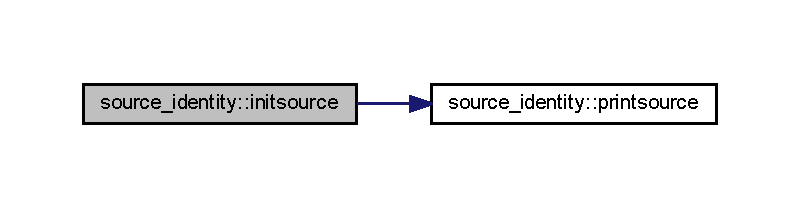
\includegraphics[width=350pt]{namespacesource__identity_a3939e59172252d0edce57e00ea41758d_cgraph}
\end{center}
\end{figure}
Here is the caller graph for this function\+:\nopagebreak
\begin{figure}[H]
\begin{center}
\leavevmode
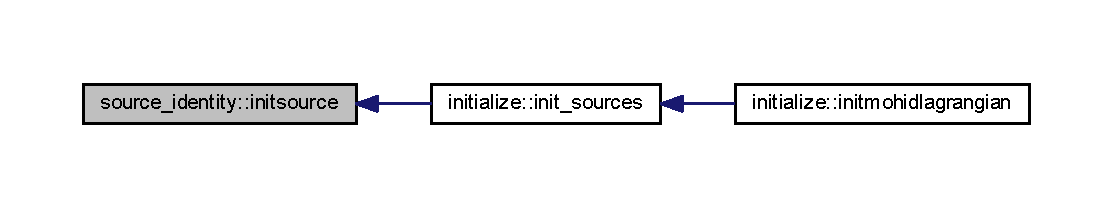
\includegraphics[width=350pt]{namespacesource__identity_a3939e59172252d0edce57e00ea41758d_icgraph}
\end{center}
\end{figure}
\mbox{\Hypertarget{namespacesource__identity_ac4fc3a54de91016023a7948d261f84a5}\label{namespacesource__identity_ac4fc3a54de91016023a7948d261f84a5}} 
\index{source\+\_\+identity@{source\+\_\+identity}!printsource@{printsource}}
\index{printsource@{printsource}!source\+\_\+identity@{source\+\_\+identity}}
\subsubsection{\texorpdfstring{printsource()}{printsource()}}
{\footnotesize\ttfamily subroutine source\+\_\+identity\+::printsource (\begin{DoxyParamCaption}\item[{type(\mbox{\hyperlink{structsource__identity_1_1source__class}{source\+\_\+class}}), intent(in)}]{src }\end{DoxyParamCaption})\hspace{0.3cm}{\ttfamily [private]}}



Birjukovs Canelas -\/ M\+A\+R\+E\+T\+EC 

source print routine -\/ prints a source info on console/log 
\begin{DoxyParams}[1]{Parameters}
\mbox{\tt in}  & {\em src} & \\
\hline
\end{DoxyParams}
Here is the caller graph for this function\+:\nopagebreak
\begin{figure}[H]
\begin{center}
\leavevmode
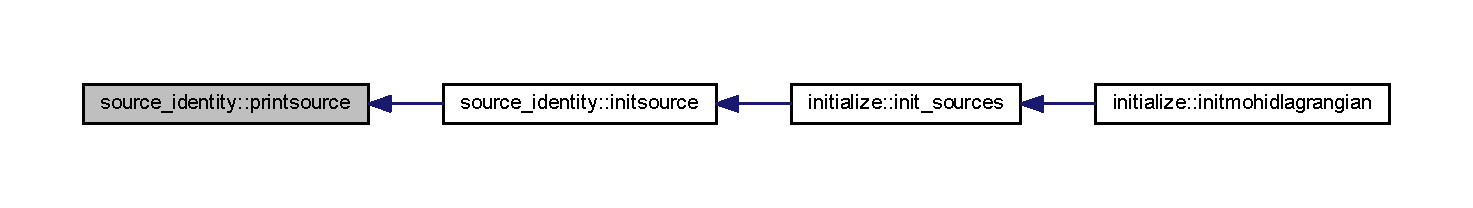
\includegraphics[width=350pt]{namespacesource__identity_ac4fc3a54de91016023a7948d261f84a5_icgraph}
\end{center}
\end{figure}


\subsection{Variable Documentation}
\mbox{\Hypertarget{namespacesource__identity_a5ed8006613af7461c6a2ff1cdaeb8f0f}\label{namespacesource__identity_a5ed8006613af7461c6a2ff1cdaeb8f0f}} 
\index{source\+\_\+identity@{source\+\_\+identity}!source@{source}}
\index{source@{source}!source\+\_\+identity@{source\+\_\+identity}}
\subsubsection{\texorpdfstring{source}{source}}
{\footnotesize\ttfamily type(\mbox{\hyperlink{structsource__identity_1_1source__class}{source\+\_\+class}}), dimension(\+:), allocatable, public source\+\_\+identity\+::source}


\hypertarget{namespacetracer}{}\section{tracer Module Reference}
\label{namespacetracer}\index{tracer@{tracer}}


Module to hold and wrap all the tracer respective modules. Defines a pure Lagrangian tracer class. This is intended to serve as the base class for every type of tracer class needed, that should be ~\newline
 built as derived of this class, with the necessary modifiers to model the desired behaviour. Basic tracer data (parameters, variables) are implemented. Tracer methods such as I/O, integration and interpolation routines are implemented.  




\subsection{Detailed Description}
Module to hold and wrap all the tracer respective modules. Defines a pure Lagrangian tracer class. This is intended to serve as the base class for every type of tracer class needed, that should be ~\newline
 built as derived of this class, with the necessary modifiers to model the desired behaviour. Basic tracer data (parameters, variables) are implemented. Tracer methods such as I/O, integration and interpolation routines are implemented. 

\begin{DoxyAuthor}{Author}
Ricardo Birjukovs Canelas 
\end{DoxyAuthor}

\hypertarget{namespacetracer2d}{}\section{tracer2d Module Reference}
\label{namespacetracer2d}\index{tracer2d@{tracer2d}}


Module that defines a pure Lagrangian 2D tracer class and related methods, as a subset of the tracer3D module.  


\subsection*{Functions/\+Subroutines}
\begin{DoxyCompactItemize}
\item 
subroutine \mbox{\hyperlink{namespacetracer2d_abebf96ac23ed37832000c68fea45f584}{tracer2d\+\_\+init}} (trc, filename, time, x, is\+\_\+sigma)
\begin{DoxyCompactList}\small\item\em Birjukovs Canelas -\/ M\+A\+R\+E\+T\+EC Routine Author Name and Affiliation. \end{DoxyCompactList}\end{DoxyCompactItemize}


\subsection{Detailed Description}
Module that defines a pure Lagrangian 2D tracer class and related methods, as a subset of the tracer3D module. 

\begin{DoxyAuthor}{Author}
Ricardo Birjukovs Canelas 
\end{DoxyAuthor}


\subsection{Function/\+Subroutine Documentation}
\mbox{\Hypertarget{namespacetracer2d_abebf96ac23ed37832000c68fea45f584}\label{namespacetracer2d_abebf96ac23ed37832000c68fea45f584}} 
\index{tracer2d@{tracer2d}!tracer2d\+\_\+init@{tracer2d\+\_\+init}}
\index{tracer2d\+\_\+init@{tracer2d\+\_\+init}!tracer2d@{tracer2d}}
\subsubsection{\texorpdfstring{tracer2d\+\_\+init()}{tracer2d\_init()}}
{\footnotesize\ttfamily subroutine tracer2d\+::tracer2d\+\_\+init (\begin{DoxyParamCaption}\item[{type(tracer\+\_\+class), intent(out)}]{trc,  }\item[{character(len=$\ast$), intent(in)}]{filename,  }\item[{real(prec\+\_\+time)}]{time,  }\item[{real(prec), dimension(\+:), intent(in)}]{x,  }\item[{logical, intent(in)}]{is\+\_\+sigma }\end{DoxyParamCaption})}



Birjukovs Canelas -\/ M\+A\+R\+E\+T\+EC Routine Author Name and Affiliation. 

Brief description of routine.

2D Tracer inititialization routine -\/ Generates a tracer collection and initializes their variables 
\begin{DoxyParams}[1]{Parameters}
\mbox{\tt out}  & {\em trc} & ~\newline
\\
\hline
\mbox{\tt in}  & {\em filename} & \\
\hline
\end{DoxyParams}

\hypertarget{namespacetracer3d}{}\section{tracer3d Module Reference}
\label{namespacetracer3d}\index{tracer3d@{tracer3d}}


Module that defines a pure Lagrangian tracer class and related methods.  


\subsection*{Functions/\+Subroutines}
\begin{DoxyCompactItemize}
\item 
subroutine, public \mbox{\hyperlink{namespacetracer3d_a42aa514ae0b5c46c797ddaaa48c49991}{tracer\+\_\+init}} (trc, id, time, x, y, z)
\begin{DoxyCompactList}\small\item\em Birjukovs Canelas -\/ M\+A\+R\+E\+T\+EC \end{DoxyCompactList}\end{DoxyCompactItemize}


\subsection{Detailed Description}
Module that defines a pure Lagrangian tracer class and related methods. 

\begin{DoxyAuthor}{Author}
Ricardo Birjukovs Canelas 
\end{DoxyAuthor}


\subsection{Function/\+Subroutine Documentation}
\mbox{\Hypertarget{namespacetracer3d_a42aa514ae0b5c46c797ddaaa48c49991}\label{namespacetracer3d_a42aa514ae0b5c46c797ddaaa48c49991}} 
\index{tracer3d@{tracer3d}!tracer\+\_\+init@{tracer\+\_\+init}}
\index{tracer\+\_\+init@{tracer\+\_\+init}!tracer3d@{tracer3d}}
\subsubsection{\texorpdfstring{tracer\+\_\+init()}{tracer\_init()}}
{\footnotesize\ttfamily subroutine, public tracer3d\+::tracer\+\_\+init (\begin{DoxyParamCaption}\item[{type(tracer\+\_\+class), intent(out)}]{trc,  }\item[{integer, intent(in)}]{id,  }\item[{real(prec\+\_\+time), intent(in)}]{time,  }\item[{real(prec), intent(in)}]{x,  }\item[{real(prec), intent(in)}]{y,  }\item[{real(prec), intent(in)}]{z }\end{DoxyParamCaption})}



Birjukovs Canelas -\/ M\+A\+R\+E\+T\+EC 

Tracer inititialization routine -\/ Generates a tracer and initializes its variables 
\begin{DoxyParams}[1]{Parameters}
\mbox{\tt out}  & {\em trc} & ~\newline
\\
\hline
\mbox{\tt in}  & {\em filename} & \\
\hline
\end{DoxyParams}

\hypertarget{namespacetracer__interp}{}\section{tracer\+\_\+interp Module Reference}
\label{namespacetracer__interp}\index{tracer\+\_\+interp@{tracer\+\_\+interp}}

\chapter{Data Type Documentation}
\hypertarget{structgeometry_1_1box}{}\section{geometry\+:\+:box Type Reference}
\label{structgeometry_1_1box}\index{geometry\+::box@{geometry\+::box}}


Type -\/ point class.  




Inheritance diagram for geometry\+:\+:box\+:\nopagebreak
\begin{figure}[H]
\begin{center}
\leavevmode
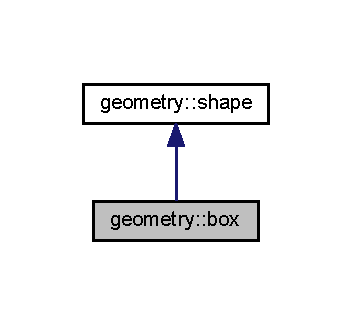
\includegraphics[width=169pt]{structgeometry_1_1box__inherit__graph}
\end{center}
\end{figure}


Collaboration diagram for geometry\+:\+:box\+:\nopagebreak
\begin{figure}[H]
\begin{center}
\leavevmode
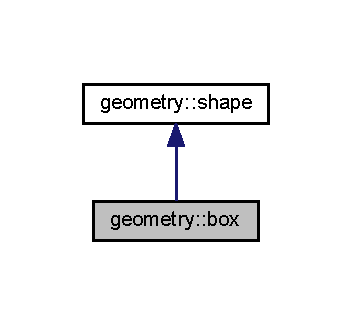
\includegraphics[width=169pt]{structgeometry_1_1box__coll__graph}
\end{center}
\end{figure}
\subsection*{Public Attributes}
\begin{DoxyCompactItemize}
\item 
type(vector) \mbox{\hyperlink{structgeometry_1_1box_a77c6ce50ff2a5d421ef59cf929f81f3d}{size}}
\begin{DoxyCompactList}\small\item\em Box size. \end{DoxyCompactList}\end{DoxyCompactItemize}


\subsection{Detailed Description}
Type -\/ point class. 

\subsection{Member Data Documentation}
\mbox{\Hypertarget{structgeometry_1_1box_a77c6ce50ff2a5d421ef59cf929f81f3d}\label{structgeometry_1_1box_a77c6ce50ff2a5d421ef59cf929f81f3d}} 
\index{geometry\+::box@{geometry\+::box}!size@{size}}
\index{size@{size}!geometry\+::box@{geometry\+::box}}
\subsubsection{\texorpdfstring{size}{size}}
{\footnotesize\ttfamily type(vector) geometry\+::box\+::size}



Box size. 



The documentation for this type was generated from the following file\+:\begin{DoxyCompactItemize}
\item 
C\+:/\+Users/administrator/\+Documents/\+Git\+Hub/\+M\+O\+H\+I\+D-\/\+Lagrangian/src/lib/\mbox{\hyperlink{geometry_8f90}{geometry.\+f90}}\end{DoxyCompactItemize}

\hypertarget{structgeometry_1_1line}{}\section{geometry\+:\+:line Type Reference}
\label{structgeometry_1_1line}\index{geometry\+::line@{geometry\+::line}}


Type -\/ line class.  




Inheritance diagram for geometry\+:\+:line\+:\nopagebreak
\begin{figure}[H]
\begin{center}
\leavevmode
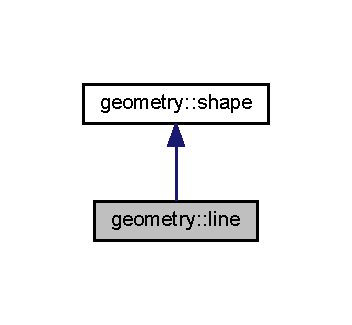
\includegraphics[width=169pt]{structgeometry_1_1line__inherit__graph}
\end{center}
\end{figure}


Collaboration diagram for geometry\+:\+:line\+:\nopagebreak
\begin{figure}[H]
\begin{center}
\leavevmode
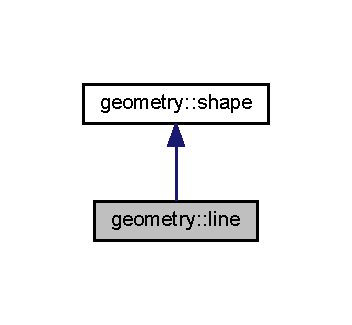
\includegraphics[width=169pt]{structgeometry_1_1line__coll__graph}
\end{center}
\end{figure}
\subsection*{Private Attributes}
\begin{DoxyCompactItemize}
\item 
type(vector) \hyperlink{structgeometry_1_1line_ab899fb3b6da58896cd14e2f1a474c457}{last}
\begin{DoxyCompactList}\small\item\em Coordinates of the end point. \end{DoxyCompactList}\end{DoxyCompactItemize}


\subsection{Detailed Description}
Type -\/ line class. 

\subsection{Member Data Documentation}
\mbox{\Hypertarget{structgeometry_1_1line_ab899fb3b6da58896cd14e2f1a474c457}\label{structgeometry_1_1line_ab899fb3b6da58896cd14e2f1a474c457}} 
\index{geometry\+::line@{geometry\+::line}!last@{last}}
\index{last@{last}!geometry\+::line@{geometry\+::line}}
\subsubsection{\texorpdfstring{last}{last}}
{\footnotesize\ttfamily type(vector) geometry\+::line\+::last\hspace{0.3cm}{\ttfamily [private]}}



Coordinates of the end point. 



The documentation for this type was generated from the following file\+:\begin{DoxyCompactItemize}
\item 
C\+:/\+Users/administrator/\+Documents/\+Git\+Hub/\+M\+O\+H\+I\+D-\/\+Lagrangian/src/lib/\hyperlink{geometry_8f90}{geometry.\+f90}\end{DoxyCompactItemize}

\hypertarget{structgeometry_1_1point}{}\section{geometry\+:\+:point Type Reference}
\label{structgeometry_1_1point}\index{geometry\+::point@{geometry\+::point}}


Type -\/ point class.  




Inheritance diagram for geometry\+:\+:point\+:\nopagebreak
\begin{figure}[H]
\begin{center}
\leavevmode
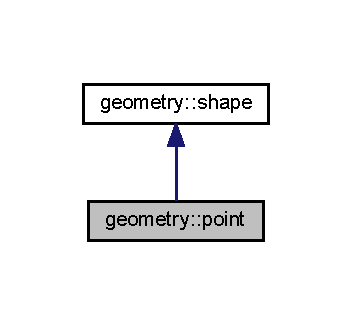
\includegraphics[width=169pt]{structgeometry_1_1point__inherit__graph}
\end{center}
\end{figure}


Collaboration diagram for geometry\+:\+:point\+:\nopagebreak
\begin{figure}[H]
\begin{center}
\leavevmode
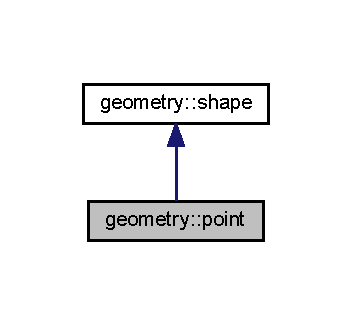
\includegraphics[width=169pt]{structgeometry_1_1point__coll__graph}
\end{center}
\end{figure}


\subsection{Detailed Description}
Type -\/ point class. 

The documentation for this type was generated from the following file\+:\begin{DoxyCompactItemize}
\item 
C\+:/\+Users/administrator/\+Documents/\+Git\+Hub/\+M\+O\+H\+I\+D-\/\+Lagrangian/src/lib/\mbox{\hyperlink{geometry_8f90}{geometry.\+f90}}\end{DoxyCompactItemize}

\hypertarget{structgeometry_1_1shape}{}\section{geometry\+:\+:shape Type Reference}
\label{structgeometry_1_1shape}\index{geometry\+::shape@{geometry\+::shape}}


Inheritance diagram for geometry\+:\+:shape\+:
% FIG 0
\subsection*{Public Attributes}
\begin{DoxyCompactItemize}
\item 
type(vector) \mbox{\hyperlink{structgeometry_1_1shape_aada595aa3503cf22350737caf2931e6a}{pt}}
\begin{DoxyCompactList}\small\item\em Type -\/ extendable shape class. \end{DoxyCompactList}\item 
type(vector) \mbox{\hyperlink{structgeometry_1_1shape_ae31a17702996581b8a7d9f0b601e426e}{coordinates}}
\item 
type(vector) \mbox{\hyperlink{structgeometry_1_1shape_a00023e2069f5764880267801959ecb30}{of}}
\item 
type(vector) \mbox{\hyperlink{structgeometry_1_1shape_a16013638e58225ff4d6ad562713d5db8}{a}}
\item 
type(vector) \mbox{\hyperlink{structgeometry_1_1shape_a56d125828996ab14b6eb030cac6d242f}{point}}
\end{DoxyCompactItemize}


\subsection{Member Data Documentation}
\mbox{\Hypertarget{structgeometry_1_1shape_a16013638e58225ff4d6ad562713d5db8}\label{structgeometry_1_1shape_a16013638e58225ff4d6ad562713d5db8}} 
\index{geometry\+::shape@{geometry\+::shape}!a@{a}}
\index{a@{a}!geometry\+::shape@{geometry\+::shape}}
\subsubsection{\texorpdfstring{a}{a}}
{\footnotesize\ttfamily type(vector) geometry\+::shape\+::a}

\mbox{\Hypertarget{structgeometry_1_1shape_ae31a17702996581b8a7d9f0b601e426e}\label{structgeometry_1_1shape_ae31a17702996581b8a7d9f0b601e426e}} 
\index{geometry\+::shape@{geometry\+::shape}!coordinates@{coordinates}}
\index{coordinates@{coordinates}!geometry\+::shape@{geometry\+::shape}}
\subsubsection{\texorpdfstring{coordinates}{coordinates}}
{\footnotesize\ttfamily type(vector) geometry\+::shape\+::coordinates}

\mbox{\Hypertarget{structgeometry_1_1shape_a00023e2069f5764880267801959ecb30}\label{structgeometry_1_1shape_a00023e2069f5764880267801959ecb30}} 
\index{geometry\+::shape@{geometry\+::shape}!of@{of}}
\index{of@{of}!geometry\+::shape@{geometry\+::shape}}
\subsubsection{\texorpdfstring{of}{of}}
{\footnotesize\ttfamily type(vector) geometry\+::shape\+::of}

\mbox{\Hypertarget{structgeometry_1_1shape_a56d125828996ab14b6eb030cac6d242f}\label{structgeometry_1_1shape_a56d125828996ab14b6eb030cac6d242f}} 
\index{geometry\+::shape@{geometry\+::shape}!point@{point}}
\index{point@{point}!geometry\+::shape@{geometry\+::shape}}
\subsubsection{\texorpdfstring{point}{point}}
{\footnotesize\ttfamily type(vector) geometry\+::shape\+::point}

\mbox{\Hypertarget{structgeometry_1_1shape_aada595aa3503cf22350737caf2931e6a}\label{structgeometry_1_1shape_aada595aa3503cf22350737caf2931e6a}} 
\index{geometry\+::shape@{geometry\+::shape}!pt@{pt}}
\index{pt@{pt}!geometry\+::shape@{geometry\+::shape}}
\subsubsection{\texorpdfstring{pt}{pt}}
{\footnotesize\ttfamily type(vector) geometry\+::shape\+::pt}



Type -\/ extendable shape class. 



The documentation for this type was generated from the following file\+:\begin{DoxyCompactItemize}
\item 
C\+:/\+Users/administrator/\+Documents/\+Git\+Hub/\+M\+O\+H\+I\+D-\/\+Lagrangian/src/lib/\mbox{\hyperlink{geometry_8f90}{geometry.\+f90}}\end{DoxyCompactItemize}

\hypertarget{structsource__identity_1_1source__class}{}\section{source\+\_\+identity\+:\+:source\+\_\+class Type Reference}
\label{structsource__identity_1_1source__class}\index{source\+\_\+identity\+::source\+\_\+class@{source\+\_\+identity\+::source\+\_\+class}}


Type -\/ The source class.  




Collaboration diagram for source\+\_\+identity\+:\+:source\+\_\+class\+:\nopagebreak
\begin{figure}[H]
\begin{center}
\leavevmode
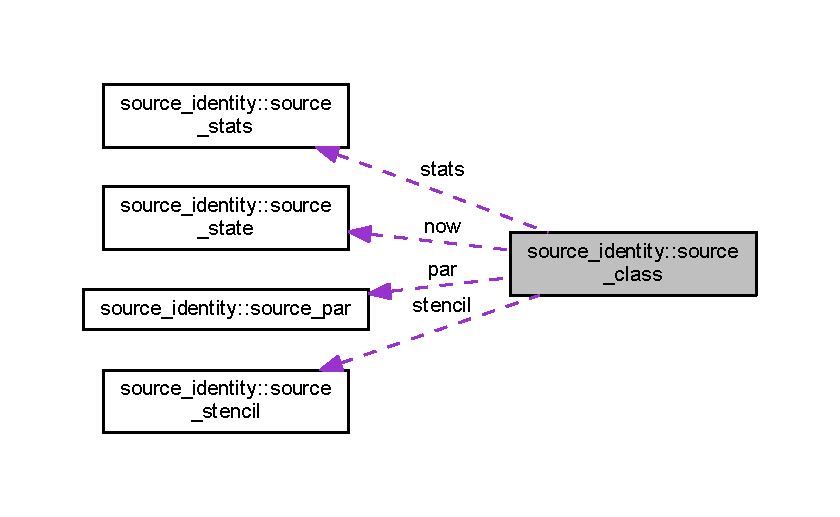
\includegraphics[width=350pt]{structsource__identity_1_1source__class__coll__graph}
\end{center}
\end{figure}
\subsection*{Private Member Functions}
\begin{DoxyCompactItemize}
\item 
procedure \mbox{\hyperlink{structsource__identity_1_1source__class_af232e5b647bcb16f34dcc2f797ef7a95}{initialize}}
\item 
procedure \mbox{\hyperlink{structsource__identity_1_1source__class_ad889c3a7ce279e199ecf059a50a73ca2}{linkproperty}}
\item 
procedure \mbox{\hyperlink{structsource__identity_1_1source__class_ac9866a62bf8838665bb929deff5bce24}{printout}}
\end{DoxyCompactItemize}
\subsection*{Private Attributes}
\begin{DoxyCompactItemize}
\item 
type(\mbox{\hyperlink{structsource__identity_1_1source__par}{source\+\_\+par}}) \mbox{\hyperlink{structsource__identity_1_1source__class_a99403ddb327779cbdbb98f15ca9116a8}{par}}
\begin{DoxyCompactList}\small\item\em To access parameters. \end{DoxyCompactList}\item 
type(\mbox{\hyperlink{structsource__identity_1_1source__state}{source\+\_\+state}}) \mbox{\hyperlink{structsource__identity_1_1source__class_a75abb328a740fa4c23201e1c311312d1}{now}}
\begin{DoxyCompactList}\small\item\em To access state variables. \end{DoxyCompactList}\item 
type(\mbox{\hyperlink{structsource__identity_1_1source__stencil}{source\+\_\+stencil}}) \mbox{\hyperlink{structsource__identity_1_1source__class_a470518874a42bab9225f3c72be0128ba}{stencil}}
\begin{DoxyCompactList}\small\item\em To acess stencil variables. \end{DoxyCompactList}\item 
type(\mbox{\hyperlink{structsource__identity_1_1source__stats}{source\+\_\+stats}}) \mbox{\hyperlink{structsource__identity_1_1source__class_a630571a5e588a6ced99787b473bf5e2f}{stats}}
\begin{DoxyCompactList}\small\item\em To access statistics. \end{DoxyCompactList}\end{DoxyCompactItemize}


\subsection{Detailed Description}
Type -\/ The source class. 

\subsection{Member Function/\+Subroutine Documentation}
\mbox{\Hypertarget{structsource__identity_1_1source__class_af232e5b647bcb16f34dcc2f797ef7a95}\label{structsource__identity_1_1source__class_af232e5b647bcb16f34dcc2f797ef7a95}} 
\index{source\+\_\+identity\+::source\+\_\+class@{source\+\_\+identity\+::source\+\_\+class}!initialize@{initialize}}
\index{initialize@{initialize}!source\+\_\+identity\+::source\+\_\+class@{source\+\_\+identity\+::source\+\_\+class}}
\subsubsection{\texorpdfstring{initialize()}{initialize()}}
{\footnotesize\ttfamily procedure source\+\_\+identity\+::source\+\_\+class\+::initialize (\begin{DoxyParamCaption}{ }\end{DoxyParamCaption})\hspace{0.3cm}{\ttfamily [private]}}

\mbox{\Hypertarget{structsource__identity_1_1source__class_ad889c3a7ce279e199ecf059a50a73ca2}\label{structsource__identity_1_1source__class_ad889c3a7ce279e199ecf059a50a73ca2}} 
\index{source\+\_\+identity\+::source\+\_\+class@{source\+\_\+identity\+::source\+\_\+class}!linkproperty@{linkproperty}}
\index{linkproperty@{linkproperty}!source\+\_\+identity\+::source\+\_\+class@{source\+\_\+identity\+::source\+\_\+class}}
\subsubsection{\texorpdfstring{linkproperty()}{linkproperty()}}
{\footnotesize\ttfamily procedure source\+\_\+identity\+::source\+\_\+class\+::linkproperty (\begin{DoxyParamCaption}{ }\end{DoxyParamCaption})\hspace{0.3cm}{\ttfamily [private]}}

\mbox{\Hypertarget{structsource__identity_1_1source__class_ac9866a62bf8838665bb929deff5bce24}\label{structsource__identity_1_1source__class_ac9866a62bf8838665bb929deff5bce24}} 
\index{source\+\_\+identity\+::source\+\_\+class@{source\+\_\+identity\+::source\+\_\+class}!printout@{printout}}
\index{printout@{printout}!source\+\_\+identity\+::source\+\_\+class@{source\+\_\+identity\+::source\+\_\+class}}
\subsubsection{\texorpdfstring{printout()}{printout()}}
{\footnotesize\ttfamily procedure source\+\_\+identity\+::source\+\_\+class\+::printout (\begin{DoxyParamCaption}{ }\end{DoxyParamCaption})\hspace{0.3cm}{\ttfamily [private]}}



\subsection{Member Data Documentation}
\mbox{\Hypertarget{structsource__identity_1_1source__class_a75abb328a740fa4c23201e1c311312d1}\label{structsource__identity_1_1source__class_a75abb328a740fa4c23201e1c311312d1}} 
\index{source\+\_\+identity\+::source\+\_\+class@{source\+\_\+identity\+::source\+\_\+class}!now@{now}}
\index{now@{now}!source\+\_\+identity\+::source\+\_\+class@{source\+\_\+identity\+::source\+\_\+class}}
\subsubsection{\texorpdfstring{now}{now}}
{\footnotesize\ttfamily type(\mbox{\hyperlink{structsource__identity_1_1source__state}{source\+\_\+state}}) source\+\_\+identity\+::source\+\_\+class\+::now\hspace{0.3cm}{\ttfamily [private]}}



To access state variables. 

\mbox{\Hypertarget{structsource__identity_1_1source__class_a99403ddb327779cbdbb98f15ca9116a8}\label{structsource__identity_1_1source__class_a99403ddb327779cbdbb98f15ca9116a8}} 
\index{source\+\_\+identity\+::source\+\_\+class@{source\+\_\+identity\+::source\+\_\+class}!par@{par}}
\index{par@{par}!source\+\_\+identity\+::source\+\_\+class@{source\+\_\+identity\+::source\+\_\+class}}
\subsubsection{\texorpdfstring{par}{par}}
{\footnotesize\ttfamily type(\mbox{\hyperlink{structsource__identity_1_1source__par}{source\+\_\+par}}) source\+\_\+identity\+::source\+\_\+class\+::par\hspace{0.3cm}{\ttfamily [private]}}



To access parameters. 

\mbox{\Hypertarget{structsource__identity_1_1source__class_a630571a5e588a6ced99787b473bf5e2f}\label{structsource__identity_1_1source__class_a630571a5e588a6ced99787b473bf5e2f}} 
\index{source\+\_\+identity\+::source\+\_\+class@{source\+\_\+identity\+::source\+\_\+class}!stats@{stats}}
\index{stats@{stats}!source\+\_\+identity\+::source\+\_\+class@{source\+\_\+identity\+::source\+\_\+class}}
\subsubsection{\texorpdfstring{stats}{stats}}
{\footnotesize\ttfamily type(\mbox{\hyperlink{structsource__identity_1_1source__stats}{source\+\_\+stats}}) source\+\_\+identity\+::source\+\_\+class\+::stats\hspace{0.3cm}{\ttfamily [private]}}



To access statistics. 

\mbox{\Hypertarget{structsource__identity_1_1source__class_a470518874a42bab9225f3c72be0128ba}\label{structsource__identity_1_1source__class_a470518874a42bab9225f3c72be0128ba}} 
\index{source\+\_\+identity\+::source\+\_\+class@{source\+\_\+identity\+::source\+\_\+class}!stencil@{stencil}}
\index{stencil@{stencil}!source\+\_\+identity\+::source\+\_\+class@{source\+\_\+identity\+::source\+\_\+class}}
\subsubsection{\texorpdfstring{stencil}{stencil}}
{\footnotesize\ttfamily type(\mbox{\hyperlink{structsource__identity_1_1source__stencil}{source\+\_\+stencil}}) source\+\_\+identity\+::source\+\_\+class\+::stencil\hspace{0.3cm}{\ttfamily [private]}}



To acess stencil variables. 



The documentation for this type was generated from the following file\+:\begin{DoxyCompactItemize}
\item 
C\+:/\+Users/administrator/\+Documents/\+Git\+Hub/\+M\+O\+H\+I\+D-\/\+Lagrangian/src/lib/\mbox{\hyperlink{source__identity_8f90}{source\+\_\+identity.\+f90}}\end{DoxyCompactItemize}

\hypertarget{structsource__identity_1_1source__par__class}{}\section{source\+\_\+identity\+:\+:source\+\_\+par\+\_\+class Type Reference}
\label{structsource__identity_1_1source__par__class}\index{source\+\_\+identity\+::source\+\_\+par\+\_\+class@{source\+\_\+identity\+::source\+\_\+par\+\_\+class}}
\subsection*{Private Attributes}
\begin{DoxyCompactItemize}
\item 
integer \mbox{\hyperlink{structsource__identity_1_1source__par__class_abde865686b1a6cfa7838aec95af3a7a1}{id}}
\begin{DoxyCompactList}\small\item\em unique source identification (integer) \end{DoxyCompactList}\item 
real(prec) \mbox{\hyperlink{structsource__identity_1_1source__par__class_a26353d5ad314f4214d45e9258412130e}{emitting\+\_\+rate}}
\begin{DoxyCompactList}\small\item\em Emitting rate of the source (Hz) \end{DoxyCompactList}\item 
type(string) \mbox{\hyperlink{structsource__identity_1_1source__par__class_a31d0608c32137ff27d27c0d5ff1b2d87}{name}}
\begin{DoxyCompactList}\small\item\em source name \end{DoxyCompactList}\item 
type(string) \mbox{\hyperlink{structsource__identity_1_1source__par__class_af8c325e348c702375d57c2c37d061e45}{property\+\_\+name}}
\begin{DoxyCompactList}\small\item\em source property name \end{DoxyCompactList}\item 
type(string) \mbox{\hyperlink{structsource__identity_1_1source__par__class_ab0cf94daa109813789aaeb280faa8dc0}{source\+\_\+geometry}}
\begin{DoxyCompactList}\small\item\em Source type \+: \textquotesingle{}point\textquotesingle{}, \textquotesingle{}line\textquotesingle{}, \textquotesingle{}sphere\textquotesingle{}, \textquotesingle{}box\textquotesingle{}. \end{DoxyCompactList}\item 
class(\mbox{\hyperlink{structgeometry_1_1shape}{shape}}), allocatable \mbox{\hyperlink{structsource__identity_1_1source__par__class_ae94237cd7ecb262db820869f2049c295}{geometry}}
\begin{DoxyCompactList}\small\item\em Source geometry. \end{DoxyCompactList}\end{DoxyCompactItemize}


\subsection{Member Data Documentation}
\mbox{\Hypertarget{structsource__identity_1_1source__par__class_a26353d5ad314f4214d45e9258412130e}\label{structsource__identity_1_1source__par__class_a26353d5ad314f4214d45e9258412130e}} 
\index{source\+\_\+identity\+::source\+\_\+par\+\_\+class@{source\+\_\+identity\+::source\+\_\+par\+\_\+class}!emitting\+\_\+rate@{emitting\+\_\+rate}}
\index{emitting\+\_\+rate@{emitting\+\_\+rate}!source\+\_\+identity\+::source\+\_\+par\+\_\+class@{source\+\_\+identity\+::source\+\_\+par\+\_\+class}}
\subsubsection{\texorpdfstring{emitting\+\_\+rate}{emitting\_rate}}
{\footnotesize\ttfamily real(prec) source\+\_\+identity\+::source\+\_\+par\+\_\+class\+::emitting\+\_\+rate\hspace{0.3cm}{\ttfamily [private]}}



Emitting rate of the source (Hz) 

\mbox{\Hypertarget{structsource__identity_1_1source__par__class_ae94237cd7ecb262db820869f2049c295}\label{structsource__identity_1_1source__par__class_ae94237cd7ecb262db820869f2049c295}} 
\index{source\+\_\+identity\+::source\+\_\+par\+\_\+class@{source\+\_\+identity\+::source\+\_\+par\+\_\+class}!geometry@{geometry}}
\index{geometry@{geometry}!source\+\_\+identity\+::source\+\_\+par\+\_\+class@{source\+\_\+identity\+::source\+\_\+par\+\_\+class}}
\subsubsection{\texorpdfstring{geometry}{geometry}}
{\footnotesize\ttfamily class(\mbox{\hyperlink{structgeometry_1_1shape}{shape}}), allocatable source\+\_\+identity\+::source\+\_\+par\+\_\+class\+::geometry\hspace{0.3cm}{\ttfamily [private]}}



Source geometry. 

\mbox{\Hypertarget{structsource__identity_1_1source__par__class_abde865686b1a6cfa7838aec95af3a7a1}\label{structsource__identity_1_1source__par__class_abde865686b1a6cfa7838aec95af3a7a1}} 
\index{source\+\_\+identity\+::source\+\_\+par\+\_\+class@{source\+\_\+identity\+::source\+\_\+par\+\_\+class}!id@{id}}
\index{id@{id}!source\+\_\+identity\+::source\+\_\+par\+\_\+class@{source\+\_\+identity\+::source\+\_\+par\+\_\+class}}
\subsubsection{\texorpdfstring{id}{id}}
{\footnotesize\ttfamily integer source\+\_\+identity\+::source\+\_\+par\+\_\+class\+::id\hspace{0.3cm}{\ttfamily [private]}}



unique source identification (integer) 

\mbox{\Hypertarget{structsource__identity_1_1source__par__class_a31d0608c32137ff27d27c0d5ff1b2d87}\label{structsource__identity_1_1source__par__class_a31d0608c32137ff27d27c0d5ff1b2d87}} 
\index{source\+\_\+identity\+::source\+\_\+par\+\_\+class@{source\+\_\+identity\+::source\+\_\+par\+\_\+class}!name@{name}}
\index{name@{name}!source\+\_\+identity\+::source\+\_\+par\+\_\+class@{source\+\_\+identity\+::source\+\_\+par\+\_\+class}}
\subsubsection{\texorpdfstring{name}{name}}
{\footnotesize\ttfamily type(string) source\+\_\+identity\+::source\+\_\+par\+\_\+class\+::name\hspace{0.3cm}{\ttfamily [private]}}



source name 

\mbox{\Hypertarget{structsource__identity_1_1source__par__class_af8c325e348c702375d57c2c37d061e45}\label{structsource__identity_1_1source__par__class_af8c325e348c702375d57c2c37d061e45}} 
\index{source\+\_\+identity\+::source\+\_\+par\+\_\+class@{source\+\_\+identity\+::source\+\_\+par\+\_\+class}!property\+\_\+name@{property\+\_\+name}}
\index{property\+\_\+name@{property\+\_\+name}!source\+\_\+identity\+::source\+\_\+par\+\_\+class@{source\+\_\+identity\+::source\+\_\+par\+\_\+class}}
\subsubsection{\texorpdfstring{property\+\_\+name}{property\_name}}
{\footnotesize\ttfamily type(string) source\+\_\+identity\+::source\+\_\+par\+\_\+class\+::property\+\_\+name\hspace{0.3cm}{\ttfamily [private]}}



source property name 

\mbox{\Hypertarget{structsource__identity_1_1source__par__class_ab0cf94daa109813789aaeb280faa8dc0}\label{structsource__identity_1_1source__par__class_ab0cf94daa109813789aaeb280faa8dc0}} 
\index{source\+\_\+identity\+::source\+\_\+par\+\_\+class@{source\+\_\+identity\+::source\+\_\+par\+\_\+class}!source\+\_\+geometry@{source\+\_\+geometry}}
\index{source\+\_\+geometry@{source\+\_\+geometry}!source\+\_\+identity\+::source\+\_\+par\+\_\+class@{source\+\_\+identity\+::source\+\_\+par\+\_\+class}}
\subsubsection{\texorpdfstring{source\+\_\+geometry}{source\_geometry}}
{\footnotesize\ttfamily type(string) source\+\_\+identity\+::source\+\_\+par\+\_\+class\+::source\+\_\+geometry\hspace{0.3cm}{\ttfamily [private]}}



Source type \+: \textquotesingle{}point\textquotesingle{}, \textquotesingle{}line\textquotesingle{}, \textquotesingle{}sphere\textquotesingle{}, \textquotesingle{}box\textquotesingle{}. 



The documentation for this type was generated from the following file\+:\begin{DoxyCompactItemize}
\item 
C\+:/\+Users/administrator/\+Documents/\+Git\+Hub/\+M\+O\+H\+I\+D-\/\+Lagrangian/src/lib/\mbox{\hyperlink{source__identity_8f90}{source\+\_\+identity.\+f90}}\end{DoxyCompactItemize}

\hypertarget{structsource__identity_1_1source__state__class}{}\section{source\+\_\+identity\+:\+:source\+\_\+state\+\_\+class Type Reference}
\label{structsource__identity_1_1source__state__class}\index{source\+\_\+identity\+::source\+\_\+state\+\_\+class@{source\+\_\+identity\+::source\+\_\+state\+\_\+class}}


Type -\/ state variables of a source object.  


\subsection*{Private Attributes}
\begin{DoxyCompactItemize}
\item 
real(prec\+\_\+time) \mbox{\hyperlink{structsource__identity_1_1source__state__class_a820dc7c568f3cb21ccb68f5fa74b2766}{age}}
\item 
logical \mbox{\hyperlink{structsource__identity_1_1source__state__class_a4f53c84cc4ecb9c9700eb5df698200d8}{active}}
\begin{DoxyCompactList}\small\item\em active switch \end{DoxyCompactList}\item 
type(vector) \mbox{\hyperlink{structsource__identity_1_1source__state__class_ae69e4ee310f6c496d8c537bc2ab5cda6}{pos}}
\begin{DoxyCompactList}\small\item\em Position of the source baricenter (m) \end{DoxyCompactList}\item 
type(vector) \mbox{\hyperlink{structsource__identity_1_1source__state__class_ad3949289a86679cb23febfe41c051e59}{vel}}
\begin{DoxyCompactList}\small\item\em Velocity of the source (m s-\/1) \end{DoxyCompactList}\item 
real(prec) \mbox{\hyperlink{structsource__identity_1_1source__state__class_a67b39860ac7d45545c522a2f3cd851e8}{depth}}
\begin{DoxyCompactList}\small\item\em Depth of the source baricenter (m) \end{DoxyCompactList}\item 
real(prec) \mbox{\hyperlink{structsource__identity_1_1source__state__class_aa6b7ef1194f4f7379e86242b4dffc03f}{t}}
\begin{DoxyCompactList}\small\item\em Temperature of the source (Celcius) \end{DoxyCompactList}\end{DoxyCompactItemize}


\subsection{Detailed Description}
Type -\/ state variables of a source object. 

\subsection{Member Data Documentation}
\mbox{\Hypertarget{structsource__identity_1_1source__state__class_a4f53c84cc4ecb9c9700eb5df698200d8}\label{structsource__identity_1_1source__state__class_a4f53c84cc4ecb9c9700eb5df698200d8}} 
\index{source\+\_\+identity\+::source\+\_\+state\+\_\+class@{source\+\_\+identity\+::source\+\_\+state\+\_\+class}!active@{active}}
\index{active@{active}!source\+\_\+identity\+::source\+\_\+state\+\_\+class@{source\+\_\+identity\+::source\+\_\+state\+\_\+class}}
\subsubsection{\texorpdfstring{active}{active}}
{\footnotesize\ttfamily logical source\+\_\+identity\+::source\+\_\+state\+\_\+class\+::active\hspace{0.3cm}{\ttfamily [private]}}



active switch 

\mbox{\Hypertarget{structsource__identity_1_1source__state__class_a820dc7c568f3cb21ccb68f5fa74b2766}\label{structsource__identity_1_1source__state__class_a820dc7c568f3cb21ccb68f5fa74b2766}} 
\index{source\+\_\+identity\+::source\+\_\+state\+\_\+class@{source\+\_\+identity\+::source\+\_\+state\+\_\+class}!age@{age}}
\index{age@{age}!source\+\_\+identity\+::source\+\_\+state\+\_\+class@{source\+\_\+identity\+::source\+\_\+state\+\_\+class}}
\subsubsection{\texorpdfstring{age}{age}}
{\footnotesize\ttfamily real(prec\+\_\+time) source\+\_\+identity\+::source\+\_\+state\+\_\+class\+::age\hspace{0.3cm}{\ttfamily [private]}}

\mbox{\Hypertarget{structsource__identity_1_1source__state__class_a67b39860ac7d45545c522a2f3cd851e8}\label{structsource__identity_1_1source__state__class_a67b39860ac7d45545c522a2f3cd851e8}} 
\index{source\+\_\+identity\+::source\+\_\+state\+\_\+class@{source\+\_\+identity\+::source\+\_\+state\+\_\+class}!depth@{depth}}
\index{depth@{depth}!source\+\_\+identity\+::source\+\_\+state\+\_\+class@{source\+\_\+identity\+::source\+\_\+state\+\_\+class}}
\subsubsection{\texorpdfstring{depth}{depth}}
{\footnotesize\ttfamily real(prec) source\+\_\+identity\+::source\+\_\+state\+\_\+class\+::depth\hspace{0.3cm}{\ttfamily [private]}}



Depth of the source baricenter (m) 

\mbox{\Hypertarget{structsource__identity_1_1source__state__class_ae69e4ee310f6c496d8c537bc2ab5cda6}\label{structsource__identity_1_1source__state__class_ae69e4ee310f6c496d8c537bc2ab5cda6}} 
\index{source\+\_\+identity\+::source\+\_\+state\+\_\+class@{source\+\_\+identity\+::source\+\_\+state\+\_\+class}!pos@{pos}}
\index{pos@{pos}!source\+\_\+identity\+::source\+\_\+state\+\_\+class@{source\+\_\+identity\+::source\+\_\+state\+\_\+class}}
\subsubsection{\texorpdfstring{pos}{pos}}
{\footnotesize\ttfamily type(vector) source\+\_\+identity\+::source\+\_\+state\+\_\+class\+::pos\hspace{0.3cm}{\ttfamily [private]}}



Position of the source baricenter (m) 

\mbox{\Hypertarget{structsource__identity_1_1source__state__class_aa6b7ef1194f4f7379e86242b4dffc03f}\label{structsource__identity_1_1source__state__class_aa6b7ef1194f4f7379e86242b4dffc03f}} 
\index{source\+\_\+identity\+::source\+\_\+state\+\_\+class@{source\+\_\+identity\+::source\+\_\+state\+\_\+class}!t@{t}}
\index{t@{t}!source\+\_\+identity\+::source\+\_\+state\+\_\+class@{source\+\_\+identity\+::source\+\_\+state\+\_\+class}}
\subsubsection{\texorpdfstring{t}{t}}
{\footnotesize\ttfamily real(prec) source\+\_\+identity\+::source\+\_\+state\+\_\+class\+::t\hspace{0.3cm}{\ttfamily [private]}}



Temperature of the source (Celcius) 

\mbox{\Hypertarget{structsource__identity_1_1source__state__class_ad3949289a86679cb23febfe41c051e59}\label{structsource__identity_1_1source__state__class_ad3949289a86679cb23febfe41c051e59}} 
\index{source\+\_\+identity\+::source\+\_\+state\+\_\+class@{source\+\_\+identity\+::source\+\_\+state\+\_\+class}!vel@{vel}}
\index{vel@{vel}!source\+\_\+identity\+::source\+\_\+state\+\_\+class@{source\+\_\+identity\+::source\+\_\+state\+\_\+class}}
\subsubsection{\texorpdfstring{vel}{vel}}
{\footnotesize\ttfamily type(vector) source\+\_\+identity\+::source\+\_\+state\+\_\+class\+::vel\hspace{0.3cm}{\ttfamily [private]}}



Velocity of the source (m s-\/1) 



The documentation for this type was generated from the following file\+:\begin{DoxyCompactItemize}
\item 
C\+:/\+Users/administrator/\+Documents/\+Git\+Hub/\+M\+O\+H\+I\+D-\/\+Lagrangian/src/lib/\mbox{\hyperlink{source__identity_8f90}{source\+\_\+identity.\+f90}}\end{DoxyCompactItemize}

\hypertarget{structsource__identity_1_1source__stats__class}{}\section{source\+\_\+identity\+:\+:source\+\_\+stats\+\_\+class Type Reference}
\label{structsource__identity_1_1source__stats__class}\index{source\+\_\+identity\+::source\+\_\+stats\+\_\+class@{source\+\_\+identity\+::source\+\_\+stats\+\_\+class}}


Type -\/ statistical variables of a source object.  


\subsection*{Private Attributes}
\begin{DoxyCompactItemize}
\item 
integer \mbox{\hyperlink{structsource__identity_1_1source__stats__class_a56ec334a178feedfc7ad55a1369fc89a}{particles\+\_\+emitted}}
\begin{DoxyCompactList}\small\item\em Number of emitted particles by this source. \end{DoxyCompactList}\item 
real(prec\+\_\+wrt) \mbox{\hyperlink{structsource__identity_1_1source__stats__class_aa5e66f9ef6c5061a25fba1c2895ee6db}{acc\+\_\+t}}
\begin{DoxyCompactList}\small\item\em Accumulated temperature of the tracer (Celcius) \end{DoxyCompactList}\item 
integer \mbox{\hyperlink{structsource__identity_1_1source__stats__class_a978883318dd2750f36ad1d6fe367dc46}{ns}}
\begin{DoxyCompactList}\small\item\em Number of sampling steps. \end{DoxyCompactList}\end{DoxyCompactItemize}


\subsection{Detailed Description}
Type -\/ statistical variables of a source object. 

\subsection{Member Data Documentation}
\mbox{\Hypertarget{structsource__identity_1_1source__stats__class_aa5e66f9ef6c5061a25fba1c2895ee6db}\label{structsource__identity_1_1source__stats__class_aa5e66f9ef6c5061a25fba1c2895ee6db}} 
\index{source\+\_\+identity\+::source\+\_\+stats\+\_\+class@{source\+\_\+identity\+::source\+\_\+stats\+\_\+class}!acc\+\_\+t@{acc\+\_\+t}}
\index{acc\+\_\+t@{acc\+\_\+t}!source\+\_\+identity\+::source\+\_\+stats\+\_\+class@{source\+\_\+identity\+::source\+\_\+stats\+\_\+class}}
\subsubsection{\texorpdfstring{acc\+\_\+t}{acc\_t}}
{\footnotesize\ttfamily real(prec\+\_\+wrt) source\+\_\+identity\+::source\+\_\+stats\+\_\+class\+::acc\+\_\+t\hspace{0.3cm}{\ttfamily [private]}}



Accumulated temperature of the tracer (Celcius) 

\mbox{\Hypertarget{structsource__identity_1_1source__stats__class_a978883318dd2750f36ad1d6fe367dc46}\label{structsource__identity_1_1source__stats__class_a978883318dd2750f36ad1d6fe367dc46}} 
\index{source\+\_\+identity\+::source\+\_\+stats\+\_\+class@{source\+\_\+identity\+::source\+\_\+stats\+\_\+class}!ns@{ns}}
\index{ns@{ns}!source\+\_\+identity\+::source\+\_\+stats\+\_\+class@{source\+\_\+identity\+::source\+\_\+stats\+\_\+class}}
\subsubsection{\texorpdfstring{ns}{ns}}
{\footnotesize\ttfamily integer source\+\_\+identity\+::source\+\_\+stats\+\_\+class\+::ns\hspace{0.3cm}{\ttfamily [private]}}



Number of sampling steps. 

\mbox{\Hypertarget{structsource__identity_1_1source__stats__class_a56ec334a178feedfc7ad55a1369fc89a}\label{structsource__identity_1_1source__stats__class_a56ec334a178feedfc7ad55a1369fc89a}} 
\index{source\+\_\+identity\+::source\+\_\+stats\+\_\+class@{source\+\_\+identity\+::source\+\_\+stats\+\_\+class}!particles\+\_\+emitted@{particles\+\_\+emitted}}
\index{particles\+\_\+emitted@{particles\+\_\+emitted}!source\+\_\+identity\+::source\+\_\+stats\+\_\+class@{source\+\_\+identity\+::source\+\_\+stats\+\_\+class}}
\subsubsection{\texorpdfstring{particles\+\_\+emitted}{particles\_emitted}}
{\footnotesize\ttfamily integer source\+\_\+identity\+::source\+\_\+stats\+\_\+class\+::particles\+\_\+emitted\hspace{0.3cm}{\ttfamily [private]}}



Number of emitted particles by this source. 



The documentation for this type was generated from the following file\+:\begin{DoxyCompactItemize}
\item 
C\+:/\+Users/administrator/\+Documents/\+Git\+Hub/\+M\+O\+H\+I\+D-\/\+Lagrangian/src/lib/\mbox{\hyperlink{source__identity_8f90}{source\+\_\+identity.\+f90}}\end{DoxyCompactItemize}

\hypertarget{structgeometry_1_1sphere}{}\section{geometry\+:\+:sphere Type Reference}
\label{structgeometry_1_1sphere}\index{geometry\+::sphere@{geometry\+::sphere}}


Type -\/ sphere class.  




Inheritance diagram for geometry\+:\+:sphere\+:\nopagebreak
\begin{figure}[H]
\begin{center}
\leavevmode
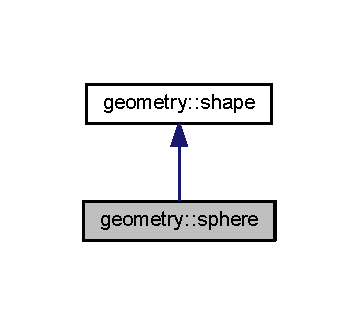
\includegraphics[width=172pt]{structgeometry_1_1sphere__inherit__graph}
\end{center}
\end{figure}


Collaboration diagram for geometry\+:\+:sphere\+:\nopagebreak
\begin{figure}[H]
\begin{center}
\leavevmode
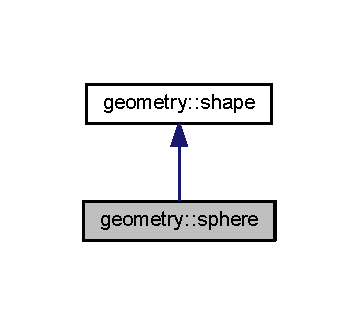
\includegraphics[width=172pt]{structgeometry_1_1sphere__coll__graph}
\end{center}
\end{figure}
\subsection*{Private Attributes}
\begin{DoxyCompactItemize}
\item 
real(prec) \hyperlink{structgeometry_1_1sphere_a906fbbdb8c6b56e7d45cea4e96b6e04d}{radius}
\begin{DoxyCompactList}\small\item\em Sphere radius. \end{DoxyCompactList}\end{DoxyCompactItemize}


\subsection{Detailed Description}
Type -\/ sphere class. 

\subsection{Member Data Documentation}
\mbox{\Hypertarget{structgeometry_1_1sphere_a906fbbdb8c6b56e7d45cea4e96b6e04d}\label{structgeometry_1_1sphere_a906fbbdb8c6b56e7d45cea4e96b6e04d}} 
\index{geometry\+::sphere@{geometry\+::sphere}!radius@{radius}}
\index{radius@{radius}!geometry\+::sphere@{geometry\+::sphere}}
\subsubsection{\texorpdfstring{radius}{radius}}
{\footnotesize\ttfamily real(prec) geometry\+::sphere\+::radius\hspace{0.3cm}{\ttfamily [private]}}



Sphere radius. 



The documentation for this type was generated from the following file\+:\begin{DoxyCompactItemize}
\item 
C\+:/\+Users/administrator/\+Documents/\+Git\+Hub/\+M\+O\+H\+I\+D-\/\+Lagrangian/src/lib/\hyperlink{geometry_8f90}{geometry.\+f90}\end{DoxyCompactItemize}

\hypertarget{structtracer3d_1_1tracer__class}{}\section{tracer3d\+:\+:tracer\+\_\+class Type Reference}
\label{structtracer3d_1_1tracer__class}\index{tracer3d\+::tracer\+\_\+class@{tracer3d\+::tracer\+\_\+class}}


Type -\/ The pure Lagrangian tracer class.  




Collaboration diagram for tracer3d\+:\+:tracer\+\_\+class\+:\nopagebreak
\begin{figure}[H]
\begin{center}
\leavevmode
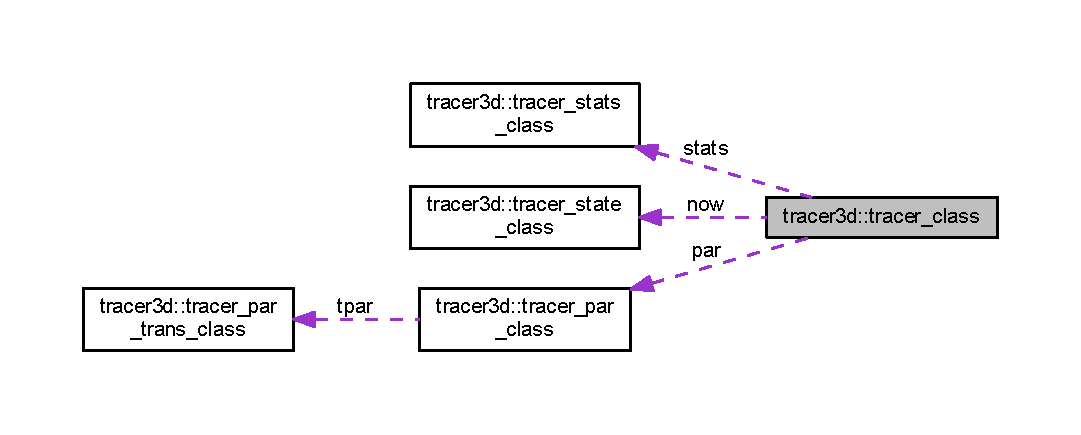
\includegraphics[width=350pt]{structtracer3d_1_1tracer__class__coll__graph}
\end{center}
\end{figure}
\subsection*{Private Attributes}
\begin{DoxyCompactItemize}
\item 
type(\mbox{\hyperlink{structtracer3d_1_1tracer__par__class}{tracer\+\_\+par\+\_\+class}}) \mbox{\hyperlink{structtracer3d_1_1tracer__class_a3745c68bd31158518852af7839b5d25d}{par}}
\begin{DoxyCompactList}\small\item\em To access parameters. \end{DoxyCompactList}\item 
type(\mbox{\hyperlink{structtracer3d_1_1tracer__state__class}{tracer\+\_\+state\+\_\+class}}) \mbox{\hyperlink{structtracer3d_1_1tracer__class_a9078a3dd8dfd7a789277f35549d31ff6}{now}}
\begin{DoxyCompactList}\small\item\em To access state variables. \end{DoxyCompactList}\item 
type(\mbox{\hyperlink{structtracer3d_1_1tracer__stats__class}{tracer\+\_\+stats\+\_\+class}}) \mbox{\hyperlink{structtracer3d_1_1tracer__class_a7145b520dad5b862da8b0fc14da0a8f0}{stats}}
\begin{DoxyCompactList}\small\item\em To access statistics. \end{DoxyCompactList}\end{DoxyCompactItemize}


\subsection{Detailed Description}
Type -\/ The pure Lagrangian tracer class. 

\subsection{Member Data Documentation}
\mbox{\Hypertarget{structtracer3d_1_1tracer__class_a9078a3dd8dfd7a789277f35549d31ff6}\label{structtracer3d_1_1tracer__class_a9078a3dd8dfd7a789277f35549d31ff6}} 
\index{tracer3d\+::tracer\+\_\+class@{tracer3d\+::tracer\+\_\+class}!now@{now}}
\index{now@{now}!tracer3d\+::tracer\+\_\+class@{tracer3d\+::tracer\+\_\+class}}
\subsubsection{\texorpdfstring{now}{now}}
{\footnotesize\ttfamily type(\mbox{\hyperlink{structtracer3d_1_1tracer__state__class}{tracer\+\_\+state\+\_\+class}}) tracer3d\+::tracer\+\_\+class\+::now\hspace{0.3cm}{\ttfamily [private]}}



To access state variables. 

\mbox{\Hypertarget{structtracer3d_1_1tracer__class_a3745c68bd31158518852af7839b5d25d}\label{structtracer3d_1_1tracer__class_a3745c68bd31158518852af7839b5d25d}} 
\index{tracer3d\+::tracer\+\_\+class@{tracer3d\+::tracer\+\_\+class}!par@{par}}
\index{par@{par}!tracer3d\+::tracer\+\_\+class@{tracer3d\+::tracer\+\_\+class}}
\subsubsection{\texorpdfstring{par}{par}}
{\footnotesize\ttfamily type(\mbox{\hyperlink{structtracer3d_1_1tracer__par__class}{tracer\+\_\+par\+\_\+class}}) tracer3d\+::tracer\+\_\+class\+::par\hspace{0.3cm}{\ttfamily [private]}}



To access parameters. 

\mbox{\Hypertarget{structtracer3d_1_1tracer__class_a7145b520dad5b862da8b0fc14da0a8f0}\label{structtracer3d_1_1tracer__class_a7145b520dad5b862da8b0fc14da0a8f0}} 
\index{tracer3d\+::tracer\+\_\+class@{tracer3d\+::tracer\+\_\+class}!stats@{stats}}
\index{stats@{stats}!tracer3d\+::tracer\+\_\+class@{tracer3d\+::tracer\+\_\+class}}
\subsubsection{\texorpdfstring{stats}{stats}}
{\footnotesize\ttfamily type(\mbox{\hyperlink{structtracer3d_1_1tracer__stats__class}{tracer\+\_\+stats\+\_\+class}}) tracer3d\+::tracer\+\_\+class\+::stats\hspace{0.3cm}{\ttfamily [private]}}



To access statistics. 



The documentation for this type was generated from the following file\+:\begin{DoxyCompactItemize}
\item 
C\+:/\+Users/administrator/\+Documents/\+Git\+Hub/\+M\+O\+H\+I\+D-\/\+Lagrangian/src/lib/\mbox{\hyperlink{tracer3_d_8f90}{tracer3\+D.\+f90}}\end{DoxyCompactItemize}

\hypertarget{structtracer3d_1_1tracer__par__class}{}\section{tracer3d\+:\+:tracer\+\_\+par\+\_\+class Type Reference}
\label{structtracer3d_1_1tracer__par__class}\index{tracer3d\+::tracer\+\_\+par\+\_\+class@{tracer3d\+::tracer\+\_\+par\+\_\+class}}
\subsection*{Public Attributes}
\begin{DoxyCompactItemize}
\item 
\mbox{\Hypertarget{structtracer3d_1_1tracer__par__class_afee9b223da2104cc94d7925a09ce1b5b}\label{structtracer3d_1_1tracer__par__class_afee9b223da2104cc94d7925a09ce1b5b}} 
integer \mbox{\hyperlink{structtracer3d_1_1tracer__par__class_afee9b223da2104cc94d7925a09ce1b5b}{n}}
\begin{DoxyCompactList}\small\item\em Type -\/ parameters of a pure Lagrangian tracer object. \end{DoxyCompactList}\item 
\mbox{\Hypertarget{structtracer3d_1_1tracer__par__class_a595e743676b4b97d7b6895ce1da701c2}\label{structtracer3d_1_1tracer__par__class_a595e743676b4b97d7b6895ce1da701c2}} 
integer {\bfseries n\+\_\+active}
\item 
\mbox{\Hypertarget{structtracer3d_1_1tracer__par__class_a88718350ee32f1a882264dd68ed377a8}\label{structtracer3d_1_1tracer__par__class_a88718350ee32f1a882264dd68ed377a8}} 
integer {\bfseries n\+\_\+max\+\_\+dep}
\item 
\mbox{\Hypertarget{structtracer3d_1_1tracer__par__class_a249769f71ff720d3ac6d594c7670f507}\label{structtracer3d_1_1tracer__par__class_a249769f71ff720d3ac6d594c7670f507}} 
integer {\bfseries id\+\_\+max}
\item 
\mbox{\Hypertarget{structtracer3d_1_1tracer__par__class_ab3070eb172aec777973175d521fde0d4}\label{structtracer3d_1_1tracer__par__class_ab3070eb172aec777973175d521fde0d4}} 
logical {\bfseries is\+\_\+sigma}
\item 
\mbox{\Hypertarget{structtracer3d_1_1tracer__par__class_a17d4f4f2e5c564cfd71aec5a9c86e9ae}\label{structtracer3d_1_1tracer__par__class_a17d4f4f2e5c564cfd71aec5a9c86e9ae}} 
real(prec\+\_\+time) {\bfseries dt}
\item 
\mbox{\Hypertarget{structtracer3d_1_1tracer__par__class_a03f19bcc6a1d85314b1e79b3339092fa}\label{structtracer3d_1_1tracer__par__class_a03f19bcc6a1d85314b1e79b3339092fa}} 
real(prec\+\_\+time) {\bfseries dt\+\_\+dep}
\item 
\mbox{\Hypertarget{structtracer3d_1_1tracer__par__class_a3c25026d05e257ab283072e7c112311b}\label{structtracer3d_1_1tracer__par__class_a3c25026d05e257ab283072e7c112311b}} 
real(prec\+\_\+time) {\bfseries dt\+\_\+write}
\item 
\mbox{\Hypertarget{structtracer3d_1_1tracer__par__class_acf2b12b8eaf5570a8f0ba0d12222269f}\label{structtracer3d_1_1tracer__par__class_acf2b12b8eaf5570a8f0ba0d12222269f}} 
real(prec) {\bfseries thk\+\_\+min}
\item 
\mbox{\Hypertarget{structtracer3d_1_1tracer__par__class_a475d343b54e274b8dfe70268f95c4d3f}\label{structtracer3d_1_1tracer__par__class_a475d343b54e274b8dfe70268f95c4d3f}} 
real(prec) {\bfseries h\+\_\+min}
\item 
\mbox{\Hypertarget{structtracer3d_1_1tracer__par__class_afff0b95b0ab6d6aad07f2bd25f74b9dc}\label{structtracer3d_1_1tracer__par__class_afff0b95b0ab6d6aad07f2bd25f74b9dc}} 
real(prec) {\bfseries depth\+\_\+max}
\item 
\mbox{\Hypertarget{structtracer3d_1_1tracer__par__class_ad0ae3a7d44261e8f378184ced0b61972}\label{structtracer3d_1_1tracer__par__class_ad0ae3a7d44261e8f378184ced0b61972}} 
real(prec) {\bfseries u\+\_\+max}
\item 
\mbox{\Hypertarget{structtracer3d_1_1tracer__par__class_a5d490688e99c3590ca3615f61da57d78}\label{structtracer3d_1_1tracer__par__class_a5d490688e99c3590ca3615f61da57d78}} 
real(prec) {\bfseries u\+\_\+max\+\_\+dep}
\item 
\mbox{\Hypertarget{structtracer3d_1_1tracer__par__class_a18eff67cc1119b68f8301a1aa78da899}\label{structtracer3d_1_1tracer__par__class_a18eff67cc1119b68f8301a1aa78da899}} 
real(prec) {\bfseries h\+\_\+min\+\_\+dep}
\item 
\mbox{\Hypertarget{structtracer3d_1_1tracer__par__class_a7784a45b39d84e70b44df3afda935acb}\label{structtracer3d_1_1tracer__par__class_a7784a45b39d84e70b44df3afda935acb}} 
real(prec) {\bfseries alpha}
\item 
\mbox{\Hypertarget{structtracer3d_1_1tracer__par__class_a4414deb31b8791b1cdf5ca5646d14225}\label{structtracer3d_1_1tracer__par__class_a4414deb31b8791b1cdf5ca5646d14225}} 
character(len=56) {\bfseries weight}
\item 
\mbox{\Hypertarget{structtracer3d_1_1tracer__par__class_af258b7ca349ce911511dbd89b24606f7}\label{structtracer3d_1_1tracer__par__class_af258b7ca349ce911511dbd89b24606f7}} 
logical {\bfseries noise}
\item 
\mbox{\Hypertarget{structtracer3d_1_1tracer__par__class_aadbc554683f144875a2a0dd60baa5450}\label{structtracer3d_1_1tracer__par__class_aadbc554683f144875a2a0dd60baa5450}} 
real(prec) {\bfseries dens\+\_\+z\+\_\+lim}
\item 
\mbox{\Hypertarget{structtracer3d_1_1tracer__par__class_a7617f9085e28d93250ebed7ad6007869}\label{structtracer3d_1_1tracer__par__class_a7617f9085e28d93250ebed7ad6007869}} 
integer {\bfseries dens\+\_\+max}
\item 
\mbox{\Hypertarget{structtracer3d_1_1tracer__par__class_a33c8edd729f2f4c19571ee04368be4e0}\label{structtracer3d_1_1tracer__par__class_a33c8edd729f2f4c19571ee04368be4e0}} 
character(len=56) {\bfseries interp\+\_\+method}
\item 
\mbox{\Hypertarget{structtracer3d_1_1tracer__par__class_a502b51714ceeed6e028b0eaea8fc41b4}\label{structtracer3d_1_1tracer__par__class_a502b51714ceeed6e028b0eaea8fc41b4}} 
character(len=512) {\bfseries par\+\_\+trans\+\_\+file}
\item 
\mbox{\Hypertarget{structtracer3d_1_1tracer__par__class_a9bb9fd6b9779087e2db2805a803ac736}\label{structtracer3d_1_1tracer__par__class_a9bb9fd6b9779087e2db2805a803ac736}} 
logical {\bfseries use\+\_\+par\+\_\+trans}
\item 
\mbox{\Hypertarget{structtracer3d_1_1tracer__par__class_a4486f0959101435f0fdeb1c845d4bbf4}\label{structtracer3d_1_1tracer__par__class_a4486f0959101435f0fdeb1c845d4bbf4}} 
type(\mbox{\hyperlink{structtracer3d_1_1tracer__par__trans__class}{tracer\+\_\+par\+\_\+trans\+\_\+class}}) {\bfseries tpar}
\end{DoxyCompactItemize}


The documentation for this type was generated from the following file\+:\begin{DoxyCompactItemize}
\item 
src/lib/tracer3\+D.\+f90\end{DoxyCompactItemize}

\hypertarget{structtracer3d_1_1tracer__par__trans__class}{}\section{tracer3d\+:\+:tracer\+\_\+par\+\_\+trans\+\_\+class Type Reference}
\label{structtracer3d_1_1tracer__par__trans__class}\index{tracer3d\+::tracer\+\_\+par\+\_\+trans\+\_\+class@{tracer3d\+::tracer\+\_\+par\+\_\+trans\+\_\+class}}
\subsection*{Public Attributes}
\begin{DoxyCompactItemize}
\item 
\mbox{\Hypertarget{structtracer3d_1_1tracer__par__trans__class_acd1f347b090a9d50fb5c248bfd5382e4}\label{structtracer3d_1_1tracer__par__trans__class_acd1f347b090a9d50fb5c248bfd5382e4}} 
integer \mbox{\hyperlink{structtracer3d_1_1tracer__par__trans__class_acd1f347b090a9d50fb5c248bfd5382e4}{nt}}
\begin{DoxyCompactList}\small\item\em Type -\/ transient parameters of a pure Lagrangian tracer object. \end{DoxyCompactList}\item 
\mbox{\Hypertarget{structtracer3d_1_1tracer__par__trans__class_acf9adabf777d904bd8b763cfeb8a4e94}\label{structtracer3d_1_1tracer__par__trans__class_acf9adabf777d904bd8b763cfeb8a4e94}} 
real(prec), dimension(\+:), allocatable {\bfseries time}
\item 
\mbox{\Hypertarget{structtracer3d_1_1tracer__par__trans__class_a62efb8dbf563d10983dfdf951d2628dc}\label{structtracer3d_1_1tracer__par__trans__class_a62efb8dbf563d10983dfdf951d2628dc}} 
real(prec), dimension(\+:), allocatable {\bfseries h\+\_\+min\+\_\+dep}
\item 
\mbox{\Hypertarget{structtracer3d_1_1tracer__par__trans__class_a076f420209f6c2ff1aa118c93c7d1506}\label{structtracer3d_1_1tracer__par__trans__class_a076f420209f6c2ff1aa118c93c7d1506}} 
real(prec), dimension(\+:), allocatable {\bfseries dt\+\_\+dep}
\item 
\mbox{\Hypertarget{structtracer3d_1_1tracer__par__trans__class_ac5403415223ceab61201747c6d141f51}\label{structtracer3d_1_1tracer__par__trans__class_ac5403415223ceab61201747c6d141f51}} 
integer, dimension(\+:), allocatable {\bfseries n\+\_\+max\+\_\+dep}
\item 
\mbox{\Hypertarget{structtracer3d_1_1tracer__par__trans__class_abd94365b132aef667b12859310a6fb3c}\label{structtracer3d_1_1tracer__par__trans__class_abd94365b132aef667b12859310a6fb3c}} 
real(prec), dimension(\+:), allocatable {\bfseries dt\+\_\+write}
\end{DoxyCompactItemize}


The documentation for this type was generated from the following file\+:\begin{DoxyCompactItemize}
\item 
src/lib/tracer3\+D.\+f90\end{DoxyCompactItemize}

\hypertarget{structtracer3d_1_1tracer__state__class}{}\section{tracer3d\+:\+:tracer\+\_\+state\+\_\+class Type Reference}
\label{structtracer3d_1_1tracer__state__class}\index{tracer3d\+::tracer\+\_\+state\+\_\+class@{tracer3d\+::tracer\+\_\+state\+\_\+class}}
\subsection*{Public Attributes}
\begin{DoxyCompactItemize}
\item 
\mbox{\Hypertarget{structtracer3d_1_1tracer__state__class_ad2c406b0c70535b9eefc6a58b5155228}\label{structtracer3d_1_1tracer__state__class_ad2c406b0c70535b9eefc6a58b5155228}} 
real(prec\+\_\+time) \mbox{\hyperlink{structtracer3d_1_1tracer__state__class_ad2c406b0c70535b9eefc6a58b5155228}{time}}
\begin{DoxyCompactList}\small\item\em Type -\/ state variables of a pure Lagrangian tracer object. \end{DoxyCompactList}\item 
\mbox{\Hypertarget{structtracer3d_1_1tracer__state__class_aff3f9a1333320499aae96ab6e0d31ded}\label{structtracer3d_1_1tracer__state__class_aff3f9a1333320499aae96ab6e0d31ded}} 
real(prec\+\_\+time) {\bfseries time\+\_\+old}
\item 
\mbox{\Hypertarget{structtracer3d_1_1tracer__state__class_a45e7a5c8c9fb20695d004397ab2ceaee}\label{structtracer3d_1_1tracer__state__class_a45e7a5c8c9fb20695d004397ab2ceaee}} 
real(prec\+\_\+time) {\bfseries time\+\_\+dep}
\item 
\mbox{\Hypertarget{structtracer3d_1_1tracer__state__class_a4778a9a01005ff19c20dbba6c081c4b9}\label{structtracer3d_1_1tracer__state__class_a4778a9a01005ff19c20dbba6c081c4b9}} 
real(prec\+\_\+time) {\bfseries time\+\_\+write}
\item 
\mbox{\Hypertarget{structtracer3d_1_1tracer__state__class_aff1762f7b19fc4480e8ab2562ccbb9e6}\label{structtracer3d_1_1tracer__state__class_aff1762f7b19fc4480e8ab2562ccbb9e6}} 
real(prec\+\_\+time) {\bfseries dt}
\item 
\mbox{\Hypertarget{structtracer3d_1_1tracer__state__class_ab350c849df637157d07b05d6df6cd035}\label{structtracer3d_1_1tracer__state__class_ab350c849df637157d07b05d6df6cd035}} 
integer, dimension(\+:), allocatable {\bfseries active}
\item 
\mbox{\Hypertarget{structtracer3d_1_1tracer__state__class_a047e35293ddbc8f44235b95db1400cc6}\label{structtracer3d_1_1tracer__state__class_a047e35293ddbc8f44235b95db1400cc6}} 
integer, dimension(\+:), allocatable {\bfseries id}
\item 
\mbox{\Hypertarget{structtracer3d_1_1tracer__state__class_a3dd71636cabb59e0138620d91b936b78}\label{structtracer3d_1_1tracer__state__class_a3dd71636cabb59e0138620d91b936b78}} 
real(prec), dimension(\+:), allocatable {\bfseries x}
\item 
\mbox{\Hypertarget{structtracer3d_1_1tracer__state__class_af37256105de6c1965ad3ec817d1793c2}\label{structtracer3d_1_1tracer__state__class_af37256105de6c1965ad3ec817d1793c2}} 
real(prec), dimension(\+:), allocatable {\bfseries y}
\item 
\mbox{\Hypertarget{structtracer3d_1_1tracer__state__class_ae68109f8656e4a460ac598a09fcd7d91}\label{structtracer3d_1_1tracer__state__class_ae68109f8656e4a460ac598a09fcd7d91}} 
real(prec), dimension(\+:), allocatable {\bfseries z}
\item 
\mbox{\Hypertarget{structtracer3d_1_1tracer__state__class_a2327dc43d8a234c7898d7d6804eb9674}\label{structtracer3d_1_1tracer__state__class_a2327dc43d8a234c7898d7d6804eb9674}} 
real(prec), dimension(\+:), allocatable {\bfseries sigma}
\item 
\mbox{\Hypertarget{structtracer3d_1_1tracer__state__class_ab91de1a2ec3332cf6ab5f694fb6c7e8b}\label{structtracer3d_1_1tracer__state__class_ab91de1a2ec3332cf6ab5f694fb6c7e8b}} 
real(prec), dimension(\+:), allocatable {\bfseries ux}
\item 
\mbox{\Hypertarget{structtracer3d_1_1tracer__state__class_ae6822a2f1d48bd274351eef5257e3757}\label{structtracer3d_1_1tracer__state__class_ae6822a2f1d48bd274351eef5257e3757}} 
real(prec), dimension(\+:), allocatable {\bfseries uy}
\item 
\mbox{\Hypertarget{structtracer3d_1_1tracer__state__class_a8379b1be1b73a1ce6737fcd332cca3dc}\label{structtracer3d_1_1tracer__state__class_a8379b1be1b73a1ce6737fcd332cca3dc}} 
real(prec), dimension(\+:), allocatable {\bfseries uz}
\item 
\mbox{\Hypertarget{structtracer3d_1_1tracer__state__class_a82dbab042574c76501610500805392c2}\label{structtracer3d_1_1tracer__state__class_a82dbab042574c76501610500805392c2}} 
real(prec), dimension(\+:), allocatable {\bfseries ax}
\item 
\mbox{\Hypertarget{structtracer3d_1_1tracer__state__class_add9d471862791f397e2788e4e14b345b}\label{structtracer3d_1_1tracer__state__class_add9d471862791f397e2788e4e14b345b}} 
real(prec), dimension(\+:), allocatable {\bfseries ay}
\item 
\mbox{\Hypertarget{structtracer3d_1_1tracer__state__class_afbe58ebc71d95db831507b307d28a5b6}\label{structtracer3d_1_1tracer__state__class_afbe58ebc71d95db831507b307d28a5b6}} 
real(prec), dimension(\+:), allocatable {\bfseries az}
\item 
\mbox{\Hypertarget{structtracer3d_1_1tracer__state__class_a1b967658f4f0a5c0d727b02be993e241}\label{structtracer3d_1_1tracer__state__class_a1b967658f4f0a5c0d727b02be993e241}} 
real(prec), dimension(\+:), allocatable {\bfseries dpth}
\item 
\mbox{\Hypertarget{structtracer3d_1_1tracer__state__class_ae5dd01566aa84508017ea302356a263b}\label{structtracer3d_1_1tracer__state__class_ae5dd01566aa84508017ea302356a263b}} 
real(prec), dimension(\+:), allocatable {\bfseries z\+\_\+srf}
\item 
\mbox{\Hypertarget{structtracer3d_1_1tracer__state__class_aba3e3096026a8e8f090c2580944fd681}\label{structtracer3d_1_1tracer__state__class_aba3e3096026a8e8f090c2580944fd681}} 
real(prec), dimension(\+:), allocatable {\bfseries thk}
\item 
\mbox{\Hypertarget{structtracer3d_1_1tracer__state__class_ae64e9e0c66c93ee01bf9fa9049c9a381}\label{structtracer3d_1_1tracer__state__class_ae64e9e0c66c93ee01bf9fa9049c9a381}} 
real(prec), dimension(\+:), allocatable {\bfseries t}
\item 
\mbox{\Hypertarget{structtracer3d_1_1tracer__state__class_a8b97bd7e1174f0b475186c6784b0d5ec}\label{structtracer3d_1_1tracer__state__class_a8b97bd7e1174f0b475186c6784b0d5ec}} 
real(prec), dimension(\+:), allocatable {\bfseries h}
\end{DoxyCompactItemize}


The documentation for this type was generated from the following file\+:\begin{DoxyCompactItemize}
\item 
src/lib/tracer3\+D.\+f90\end{DoxyCompactItemize}

\hypertarget{structtracer3d_1_1tracer__stats__class}{}\section{tracer3d\+:\+:tracer\+\_\+stats\+\_\+class Type Reference}
\label{structtracer3d_1_1tracer__stats__class}\index{tracer3d\+::tracer\+\_\+stats\+\_\+class@{tracer3d\+::tracer\+\_\+stats\+\_\+class}}


Type -\/ statistical variables of a pure Lagrangian tracer object.  


\subsection*{Private Attributes}
\begin{DoxyCompactItemize}
\item 
type(vector) \mbox{\hyperlink{structtracer3d_1_1tracer__stats__class_a1a9df2788c632bb2dcba4e303dc83e78}{acc\+\_\+pos}}
\begin{DoxyCompactList}\small\item\em Accumulated position of the tracer (m) \end{DoxyCompactList}\item 
type(vector) \mbox{\hyperlink{structtracer3d_1_1tracer__stats__class_a623f27a49b6e37a3e5c21b8bab55a323}{acc\+\_\+vel}}
\begin{DoxyCompactList}\small\item\em Accumulated velocity of the tracer (m s-\/1) \end{DoxyCompactList}\item 
real(prec\+\_\+wrt) \mbox{\hyperlink{structtracer3d_1_1tracer__stats__class_af9e6304d89967e9ade6b1188101391b6}{acc\+\_\+depth}}
\begin{DoxyCompactList}\small\item\em Accumulated depth of the tracer (m) \end{DoxyCompactList}\item 
real(prec\+\_\+wrt) \mbox{\hyperlink{structtracer3d_1_1tracer__stats__class_acdca78550575d7690eb26482ed75aeef}{acc\+\_\+t}}
\begin{DoxyCompactList}\small\item\em Accumulated temperature of the tracer (Celcius) \end{DoxyCompactList}\item 
integer \mbox{\hyperlink{structtracer3d_1_1tracer__stats__class_a0a07132ada5734cd6f132bc9ffd327b2}{ns}}
\begin{DoxyCompactList}\small\item\em Number of sampling steps. \end{DoxyCompactList}\end{DoxyCompactItemize}


\subsection{Detailed Description}
Type -\/ statistical variables of a pure Lagrangian tracer object. 

\subsection{Member Data Documentation}
\mbox{\Hypertarget{structtracer3d_1_1tracer__stats__class_af9e6304d89967e9ade6b1188101391b6}\label{structtracer3d_1_1tracer__stats__class_af9e6304d89967e9ade6b1188101391b6}} 
\index{tracer3d\+::tracer\+\_\+stats\+\_\+class@{tracer3d\+::tracer\+\_\+stats\+\_\+class}!acc\+\_\+depth@{acc\+\_\+depth}}
\index{acc\+\_\+depth@{acc\+\_\+depth}!tracer3d\+::tracer\+\_\+stats\+\_\+class@{tracer3d\+::tracer\+\_\+stats\+\_\+class}}
\subsubsection{\texorpdfstring{acc\+\_\+depth}{acc\_depth}}
{\footnotesize\ttfamily real(prec\+\_\+wrt) tracer3d\+::tracer\+\_\+stats\+\_\+class\+::acc\+\_\+depth\hspace{0.3cm}{\ttfamily [private]}}



Accumulated depth of the tracer (m) 

\mbox{\Hypertarget{structtracer3d_1_1tracer__stats__class_a1a9df2788c632bb2dcba4e303dc83e78}\label{structtracer3d_1_1tracer__stats__class_a1a9df2788c632bb2dcba4e303dc83e78}} 
\index{tracer3d\+::tracer\+\_\+stats\+\_\+class@{tracer3d\+::tracer\+\_\+stats\+\_\+class}!acc\+\_\+pos@{acc\+\_\+pos}}
\index{acc\+\_\+pos@{acc\+\_\+pos}!tracer3d\+::tracer\+\_\+stats\+\_\+class@{tracer3d\+::tracer\+\_\+stats\+\_\+class}}
\subsubsection{\texorpdfstring{acc\+\_\+pos}{acc\_pos}}
{\footnotesize\ttfamily type(vector) tracer3d\+::tracer\+\_\+stats\+\_\+class\+::acc\+\_\+pos\hspace{0.3cm}{\ttfamily [private]}}



Accumulated position of the tracer (m) 

\mbox{\Hypertarget{structtracer3d_1_1tracer__stats__class_acdca78550575d7690eb26482ed75aeef}\label{structtracer3d_1_1tracer__stats__class_acdca78550575d7690eb26482ed75aeef}} 
\index{tracer3d\+::tracer\+\_\+stats\+\_\+class@{tracer3d\+::tracer\+\_\+stats\+\_\+class}!acc\+\_\+t@{acc\+\_\+t}}
\index{acc\+\_\+t@{acc\+\_\+t}!tracer3d\+::tracer\+\_\+stats\+\_\+class@{tracer3d\+::tracer\+\_\+stats\+\_\+class}}
\subsubsection{\texorpdfstring{acc\+\_\+t}{acc\_t}}
{\footnotesize\ttfamily real(prec\+\_\+wrt) tracer3d\+::tracer\+\_\+stats\+\_\+class\+::acc\+\_\+t\hspace{0.3cm}{\ttfamily [private]}}



Accumulated temperature of the tracer (Celcius) 

\mbox{\Hypertarget{structtracer3d_1_1tracer__stats__class_a623f27a49b6e37a3e5c21b8bab55a323}\label{structtracer3d_1_1tracer__stats__class_a623f27a49b6e37a3e5c21b8bab55a323}} 
\index{tracer3d\+::tracer\+\_\+stats\+\_\+class@{tracer3d\+::tracer\+\_\+stats\+\_\+class}!acc\+\_\+vel@{acc\+\_\+vel}}
\index{acc\+\_\+vel@{acc\+\_\+vel}!tracer3d\+::tracer\+\_\+stats\+\_\+class@{tracer3d\+::tracer\+\_\+stats\+\_\+class}}
\subsubsection{\texorpdfstring{acc\+\_\+vel}{acc\_vel}}
{\footnotesize\ttfamily type(vector) tracer3d\+::tracer\+\_\+stats\+\_\+class\+::acc\+\_\+vel\hspace{0.3cm}{\ttfamily [private]}}



Accumulated velocity of the tracer (m s-\/1) 

\mbox{\Hypertarget{structtracer3d_1_1tracer__stats__class_a0a07132ada5734cd6f132bc9ffd327b2}\label{structtracer3d_1_1tracer__stats__class_a0a07132ada5734cd6f132bc9ffd327b2}} 
\index{tracer3d\+::tracer\+\_\+stats\+\_\+class@{tracer3d\+::tracer\+\_\+stats\+\_\+class}!ns@{ns}}
\index{ns@{ns}!tracer3d\+::tracer\+\_\+stats\+\_\+class@{tracer3d\+::tracer\+\_\+stats\+\_\+class}}
\subsubsection{\texorpdfstring{ns}{ns}}
{\footnotesize\ttfamily integer tracer3d\+::tracer\+\_\+stats\+\_\+class\+::ns\hspace{0.3cm}{\ttfamily [private]}}



Number of sampling steps. 



The documentation for this type was generated from the following file\+:\begin{DoxyCompactItemize}
\item 
C\+:/\+Users/administrator/\+Documents/\+Git\+Hub/\+M\+O\+H\+I\+D-\/\+Lagrangian/src/lib/\mbox{\hyperlink{tracer3_d_8f90}{tracer3\+D.\+f90}}\end{DoxyCompactItemize}

\chapter{File Documentation}
\hypertarget{main_8f90}{}\section{C\+:/\+Users/administrator/\+Documents/\+Git\+Hub/\+M\+O\+H\+I\+D-\/\+Lagrangian/src/app/main.f90 File Reference}
\label{main_8f90}\index{C\+:/\+Users/administrator/\+Documents/\+Git\+Hub/\+M\+O\+H\+I\+D-\/\+Lagrangian/src/app/main.\+f90@{C\+:/\+Users/administrator/\+Documents/\+Git\+Hub/\+M\+O\+H\+I\+D-\/\+Lagrangian/src/app/main.\+f90}}

\hypertarget{common__modules_8f90}{}\section{C\+:/\+Users/administrator/\+Documents/\+Git\+Hub/\+M\+O\+H\+I\+D-\/\+Lagrangian/src/lib/common\+\_\+modules.f90 File Reference}
\label{common__modules_8f90}\index{C\+:/\+Users/administrator/\+Documents/\+Git\+Hub/\+M\+O\+H\+I\+D-\/\+Lagrangian/src/lib/common\+\_\+modules.\+f90@{C\+:/\+Users/administrator/\+Documents/\+Git\+Hub/\+M\+O\+H\+I\+D-\/\+Lagrangian/src/lib/common\+\_\+modules.\+f90}}
\subsection*{Modules}
\begin{DoxyCompactItemize}
\item 
module \mbox{\hyperlink{namespacecommon__modules}{common\+\_\+modules}}
\begin{DoxyCompactList}\small\item\em Module to hold all of the commonly used base modules. \end{DoxyCompactList}\end{DoxyCompactItemize}

\hypertarget{geometry_8f90}{}\section{C\+:/\+Users/administrator/\+Documents/\+Git\+Hub/\+M\+O\+H\+I\+D-\/\+Lagrangian/src/lib/geometry.f90 File Reference}
\label{geometry_8f90}\index{C\+:/\+Users/administrator/\+Documents/\+Git\+Hub/\+M\+O\+H\+I\+D-\/\+Lagrangian/src/lib/geometry.\+f90@{C\+:/\+Users/administrator/\+Documents/\+Git\+Hub/\+M\+O\+H\+I\+D-\/\+Lagrangian/src/lib/geometry.\+f90}}
\subsection*{Data Types}
\begin{DoxyCompactItemize}
\item 
type \mbox{\hyperlink{structgeometry__mod_1_1geometry__class}{geometry\+\_\+mod\+::geometry\+\_\+class}}
\item 
type \mbox{\hyperlink{structgeometry__mod_1_1shape}{geometry\+\_\+mod\+::shape}}
\begin{DoxyCompactList}\small\item\em Type -\/ extendable shape class. \end{DoxyCompactList}\item 
type \mbox{\hyperlink{structgeometry__mod_1_1point}{geometry\+\_\+mod\+::point}}
\begin{DoxyCompactList}\small\item\em Type -\/ point class. \end{DoxyCompactList}\item 
type \mbox{\hyperlink{structgeometry__mod_1_1line}{geometry\+\_\+mod\+::line}}
\begin{DoxyCompactList}\small\item\em Type -\/ line class. \end{DoxyCompactList}\item 
type \mbox{\hyperlink{structgeometry__mod_1_1sphere}{geometry\+\_\+mod\+::sphere}}
\begin{DoxyCompactList}\small\item\em Type -\/ sphere class. \end{DoxyCompactList}\item 
type \mbox{\hyperlink{structgeometry__mod_1_1box}{geometry\+\_\+mod\+::box}}
\begin{DoxyCompactList}\small\item\em Type -\/ point class. \end{DoxyCompactList}\end{DoxyCompactItemize}
\subsection*{Modules}
\begin{DoxyCompactItemize}
\item 
module \mbox{\hyperlink{namespacegeometry__mod}{geometry\+\_\+mod}}
\begin{DoxyCompactList}\small\item\em Module that defines geometry classes and related methods. \end{DoxyCompactList}\end{DoxyCompactItemize}
\subsection*{Functions/\+Subroutines}
\begin{DoxyCompactItemize}
\item 
subroutine \mbox{\hyperlink{namespacegeometry__mod_a1b6f259b0b6be71e02ffae7670f7d8ba}{geometry\+\_\+mod\+::allocatelist}} (self)
\begin{DoxyCompactList}\small\item\em Public routine to allocate the possible geometry name list. \end{DoxyCompactList}\item 
logical function \mbox{\hyperlink{namespacegeometry__mod_a22dd77024fce56da299445a697256155}{geometry\+\_\+mod\+::inlist}} (self, geomname)
\begin{DoxyCompactList}\small\item\em Public function that returns a logical if the input geometry name is valid. \end{DoxyCompactList}\item 
integer function \mbox{\hyperlink{namespacegeometry__mod_ad790edd694561b33dad20cfa3a14e8f2}{geometry\+\_\+mod\+::fillsize}} (self, shapetype, dp)
\begin{DoxyCompactList}\small\item\em method to get the number of points that fill a given geometry \end{DoxyCompactList}\item 
subroutine \mbox{\hyperlink{namespacegeometry__mod_a1d97564e04562532b5389bfb91aa676b}{geometry\+\_\+mod\+::fill}} (self, shapetype, dp, fillsize, ptlist)
\begin{DoxyCompactList}\small\item\em method to get the list of points that fill a given geometry \end{DoxyCompactList}\item 
type(vector) function \mbox{\hyperlink{namespacegeometry__mod_a4a38edbff02aa0ff5f16a16c39bf778e}{geometry\+\_\+mod\+::getcenter}} (self, shapetype)
\begin{DoxyCompactList}\small\item\em method to get the baricenter of a given geometry \end{DoxyCompactList}\item 
type(vector) function, dimension(\+:), allocatable \mbox{\hyperlink{namespacegeometry__mod_a0b1a3c5aa414292ace34d59487082e3a}{geometry\+\_\+mod\+::getpoints}} (self, shapetype)
\begin{DoxyCompactList}\small\item\em method that returns the points defining a given geometry \end{DoxyCompactList}\item 
integer function \mbox{\hyperlink{namespacegeometry__mod_a524c5d28a80fb6729b102126485605ce}{geometry\+\_\+mod\+::getnumpoints}} (self, shapetype)
\begin{DoxyCompactList}\small\item\em method the points defining a given geometry \end{DoxyCompactList}\item 
subroutine \mbox{\hyperlink{namespacegeometry__mod_aed4426181ca851b41717edd50268e5f3}{geometry\+\_\+mod\+::printgeometry}} (self, shapetype)
\begin{DoxyCompactList}\small\item\em method to print the details of a given geometry \end{DoxyCompactList}\item 
integer function \mbox{\hyperlink{namespacegeometry__mod_a05de7940b4e7df5a2b31f3d0414e3743}{geometry\+\_\+mod\+::sphere\+\_\+np\+\_\+count}} (dp, r)
\begin{DoxyCompactList}\small\item\em private function that returns the number of points distributed on a grid with spacing dp inside a sphere \end{DoxyCompactList}\item 
subroutine \mbox{\hyperlink{namespacegeometry__mod_a6c03a4ea3de6763940396dbeb3908ebc}{geometry\+\_\+mod\+::sphere\+\_\+grid}} (dp, r, np, ptlist)
\begin{DoxyCompactList}\small\item\em private routine that returns the points distributed on a grid with spacing dp inside a sphere \end{DoxyCompactList}\item 
subroutine \mbox{\hyperlink{namespacegeometry__mod_ae87e4ecff2d21a839da2b82919b5fd0b}{geometry\+\_\+mod\+::box\+\_\+grid}} (dp, size, np, ptlist)
\begin{DoxyCompactList}\small\item\em private routine that returns the points distributed on a grid with spacing dp inside a box ~\newline
 \end{DoxyCompactList}\item 
subroutine \mbox{\hyperlink{namespacegeometry__mod_abcb09c0f5274c27cb79b0dd009ed94b3}{geometry\+\_\+mod\+::line\+\_\+grid}} (dp, dist, np, ptlist)
\begin{DoxyCompactList}\small\item\em private routine that returns the points distributed on a grid with spacing dp along a line ~\newline
 \end{DoxyCompactList}\end{DoxyCompactItemize}
\subsection*{Variables}
\begin{DoxyCompactItemize}
\item 
type(geometry\+\_\+class), public \mbox{\hyperlink{namespacegeometry__mod_ad2ad4f7e1138beaad5f37d5c15b7b457}{geometry\+\_\+mod\+::geometry}}
\end{DoxyCompactItemize}

\hypertarget{initialize_8f90}{}\section{C\+:/\+Users/administrator/\+Documents/\+Git\+Hub/\+M\+O\+H\+I\+D-\/\+Lagrangian/src/lib/initialize.f90 File Reference}
\label{initialize_8f90}\index{C\+:/\+Users/administrator/\+Documents/\+Git\+Hub/\+M\+O\+H\+I\+D-\/\+Lagrangian/src/lib/initialize.\+f90@{C\+:/\+Users/administrator/\+Documents/\+Git\+Hub/\+M\+O\+H\+I\+D-\/\+Lagrangian/src/lib/initialize.\+f90}}
\subsection*{Modules}
\begin{DoxyCompactItemize}
\item 
module \mbox{\hyperlink{namespaceinitialize__mod}{initialize\+\_\+mod}}
\begin{DoxyCompactList}\small\item\em Module with the simulation initialization related definitions and methods. Has one public access routine that is incharge of building the simulation space from input files. \end{DoxyCompactList}\end{DoxyCompactItemize}
\subsection*{Functions/\+Subroutines}
\begin{DoxyCompactItemize}
\item 
subroutine \mbox{\hyperlink{namespaceinitialize__mod_af38ade977df8d56db1d125bc4cc03a4a}{initialize\+\_\+mod\+::linkpropertysources}} (links\+Node)
\begin{DoxyCompactList}\small\item\em Private property xml parser routine. Reads the properties tab from the xml file and links these to the corresponding source. \end{DoxyCompactList}\item 
subroutine \mbox{\hyperlink{namespaceinitialize__mod_a4c7a93dca8bb7b573e91f877033ab22a}{initialize\+\_\+mod\+::init\+\_\+properties}} (case\+\_\+node)
\begin{DoxyCompactList}\small\item\em Private property xml parser routine. Reads the properties tab from the xml file and links these to the corresponding source. \end{DoxyCompactList}\item 
subroutine \mbox{\hyperlink{namespaceinitialize__mod_aebe8236f74bc6665b16463683c478602}{initialize\+\_\+mod\+::read\+\_\+xml\+\_\+geometry}} (source, source\+\_\+detail, source\+\_\+shape)
\begin{DoxyCompactList}\small\item\em Private geometry xml parser routine. Reads a geometry from the xml depending on the geometry type of the node. \end{DoxyCompactList}\item 
subroutine \mbox{\hyperlink{namespaceinitialize__mod_aae6a35bca190cdf65a6146f254264cd1}{initialize\+\_\+mod\+::init\+\_\+sources}} (case\+\_\+node)
\begin{DoxyCompactList}\small\item\em Private source definitions parser routine. Builds the tracer sources from the input xml case file. \end{DoxyCompactList}\item 
subroutine \mbox{\hyperlink{namespaceinitialize__mod_a18736cca205403067232125b8e510ab2}{initialize\+\_\+mod\+::init\+\_\+simdefs}} (case\+\_\+node)
\begin{DoxyCompactList}\small\item\em Private simulation definitions parser routine. Builds the simulation geometric space from the input xml case file. \end{DoxyCompactList}\item 
subroutine \mbox{\hyperlink{namespaceinitialize__mod_a9d19665b9ac12c3db8b0842bfdb6fa0c}{initialize\+\_\+mod\+::init\+\_\+caseconstants}} (case\+\_\+node)
\begin{DoxyCompactList}\small\item\em Private case constant parser routine. Builds the simulation parametric space from the input xml case file. \end{DoxyCompactList}\item 
subroutine \mbox{\hyperlink{namespaceinitialize__mod_aac9d9dabb797c83e360f9ae60a7e65e3}{initialize\+\_\+mod\+::init\+\_\+parameters}} (execution\+\_\+node)
\begin{DoxyCompactList}\small\item\em Private parameter parser routine. Builds the simulation parametric space from the input xml case file. \end{DoxyCompactList}\item 
subroutine, public \mbox{\hyperlink{namespaceinitialize__mod_a107012ffec69fe2d7c524d240193439e}{initialize\+\_\+mod\+::initfromxml}} (xmlfilename)
\begin{DoxyCompactList}\small\item\em Public xml parser routine. Builds the simulation space from the input xml case file. \end{DoxyCompactList}\end{DoxyCompactItemize}

\hypertarget{simulation__globals_8f90}{}\section{C\+:/\+Users/administrator/\+Documents/\+Git\+Hub/\+M\+O\+H\+I\+D-\/\+Lagrangian/src/lib/simulation\+\_\+globals.f90 File Reference}
\label{simulation__globals_8f90}\index{C\+:/\+Users/administrator/\+Documents/\+Git\+Hub/\+M\+O\+H\+I\+D-\/\+Lagrangian/src/lib/simulation\+\_\+globals.\+f90@{C\+:/\+Users/administrator/\+Documents/\+Git\+Hub/\+M\+O\+H\+I\+D-\/\+Lagrangian/src/lib/simulation\+\_\+globals.\+f90}}
\subsection*{Data Types}
\begin{DoxyCompactItemize}
\item 
type \hyperlink{structsimulation__globals__mod_1_1parameters__t}{simulation\+\_\+globals\+\_\+mod\+::parameters\+\_\+t}
\item 
type \hyperlink{structsimulation__globals__mod_1_1simdefs__t}{simulation\+\_\+globals\+\_\+mod\+::simdefs\+\_\+t}
\begin{DoxyCompactList}\small\item\em Simulation definitions class. \end{DoxyCompactList}\item 
type \hyperlink{structsimulation__globals__mod_1_1constants__t}{simulation\+\_\+globals\+\_\+mod\+::constants\+\_\+t}
\begin{DoxyCompactList}\small\item\em Case Constants class. \end{DoxyCompactList}\item 
type \hyperlink{structsimulation__globals__mod_1_1filenames__t}{simulation\+\_\+globals\+\_\+mod\+::filenames\+\_\+t}
\begin{DoxyCompactList}\small\item\em File names class. \end{DoxyCompactList}\item 
type \hyperlink{structsimulation__globals__mod_1_1globals__class}{simulation\+\_\+globals\+\_\+mod\+::globals\+\_\+class}
\begin{DoxyCompactList}\small\item\em Globals class -\/ This is a container for every global variable on the simulation. \end{DoxyCompactList}\end{DoxyCompactItemize}
\subsection*{Modules}
\begin{DoxyCompactItemize}
\item 
module \hyperlink{namespacesimulation__globals__mod}{simulation\+\_\+globals\+\_\+mod}
\begin{DoxyCompactList}\small\item\em Module to hold the simulation global parameter classes and their methods. \end{DoxyCompactList}\end{DoxyCompactItemize}
\subsection*{Functions/\+Subroutines}
\begin{DoxyCompactItemize}
\item 
subroutine \hyperlink{namespacesimulation__globals__mod_ac2ac06271de377004c67b6ba2f3ed353}{simulation\+\_\+globals\+\_\+mod\+::setdefaults} (self)
\begin{DoxyCompactList}\small\item\em Birjukovs Canelas -\/ M\+A\+R\+E\+T\+EC \end{DoxyCompactList}\item 
subroutine \hyperlink{namespacesimulation__globals__mod_a8a05831d4c3e3eb5741d65978f6fcf61}{simulation\+\_\+globals\+\_\+mod\+::setparameter} (self, parmkey, parmvalue)
\begin{DoxyCompactList}\small\item\em Birjukovs Canelas -\/ M\+A\+R\+E\+T\+EC \end{DoxyCompactList}\item 
subroutine \hyperlink{namespacesimulation__globals__mod_a41249abb5c33ef9e8bff448f0b3826fa}{simulation\+\_\+globals\+\_\+mod\+::check} (self)
\begin{DoxyCompactList}\small\item\em Birjukovs Canelas -\/ M\+A\+R\+E\+T\+EC \end{DoxyCompactList}\item 
subroutine \hyperlink{namespacesimulation__globals__mod_a97c04d0289a9f2d004a9329cb7ab16f0}{simulation\+\_\+globals\+\_\+mod\+::printsimparameters} (self)
\begin{DoxyCompactList}\small\item\em Birjukovs Canelas -\/ M\+A\+R\+E\+T\+EC \end{DoxyCompactList}\item 
subroutine \hyperlink{namespacesimulation__globals__mod_a68e871ed8e5d3930884e968c6fdafddc}{simulation\+\_\+globals\+\_\+mod\+::getintegratorname} (name, code)
\begin{DoxyCompactList}\small\item\em Birjukovs Canelas -\/ M\+A\+R\+E\+T\+EC \end{DoxyCompactList}\item 
subroutine \hyperlink{namespacesimulation__globals__mod_a9e92dfed4ef7388208adce768f064554}{simulation\+\_\+globals\+\_\+mod\+::setgravity} (self, grav)
\begin{DoxyCompactList}\small\item\em Birjukovs Canelas -\/ M\+A\+R\+E\+T\+EC \end{DoxyCompactList}\item 
subroutine \hyperlink{namespacesimulation__globals__mod_a64b1d91147c1cd5898fec8f23d56a65d}{simulation\+\_\+globals\+\_\+mod\+::setz0} (self, read\+\_\+z0)
\begin{DoxyCompactList}\small\item\em Birjukovs Canelas -\/ M\+A\+R\+E\+T\+EC \end{DoxyCompactList}\item 
subroutine \hyperlink{namespacesimulation__globals__mod_a68a87c39cf88bad353e28e367a721ed4}{simulation\+\_\+globals\+\_\+mod\+::setrho} (self, read\+\_\+rho)
\begin{DoxyCompactList}\small\item\em Birjukovs Canelas -\/ M\+A\+R\+E\+T\+EC \end{DoxyCompactList}\item 
subroutine \hyperlink{namespacesimulation__globals__mod_a20ba28d72a9bea823d9373a94f97026e}{simulation\+\_\+globals\+\_\+mod\+::printconstants} (self)
\begin{DoxyCompactList}\small\item\em Birjukovs Canelas -\/ M\+A\+R\+E\+T\+EC \end{DoxyCompactList}\item 
subroutine \hyperlink{namespacesimulation__globals__mod_acb8e3762572266b40a0deb166dded33a}{simulation\+\_\+globals\+\_\+mod\+::setdp} (self, read\+\_\+dp)
\begin{DoxyCompactList}\small\item\em Birjukovs Canelas -\/ M\+A\+R\+E\+T\+EC \end{DoxyCompactList}\item 
subroutine \hyperlink{namespacesimulation__globals__mod_aecf75eeccef4eeae6d10ab26cf2dcfcf}{simulation\+\_\+globals\+\_\+mod\+::setdt} (self, read\+\_\+dt)
\begin{DoxyCompactList}\small\item\em Birjukovs Canelas -\/ M\+A\+R\+E\+T\+EC \end{DoxyCompactList}\item 
subroutine \hyperlink{namespacesimulation__globals__mod_a412b0779703630189e2ea14e4b390864}{simulation\+\_\+globals\+\_\+mod\+::setboundingbox} (self, point\+\_\+, coords)
\begin{DoxyCompactList}\small\item\em Birjukovs Canelas -\/ M\+A\+R\+E\+T\+EC \end{DoxyCompactList}\item 
subroutine \hyperlink{namespacesimulation__globals__mod_aa65b43534d2d2b6366a4ebc791194805}{simulation\+\_\+globals\+\_\+mod\+::setblocksize} (self, bsize)
\begin{DoxyCompactList}\small\item\em Birjukovs Canelas -\/ M\+A\+R\+E\+T\+EC \end{DoxyCompactList}\item 
subroutine \hyperlink{namespacesimulation__globals__mod_ad331ccf019de7ed531e37c655600f90f}{simulation\+\_\+globals\+\_\+mod\+::printsimdefs} (self)
\begin{DoxyCompactList}\small\item\em Birjukovs Canelas -\/ M\+A\+R\+E\+T\+EC \end{DoxyCompactList}\end{DoxyCompactItemize}
\subsection*{Variables}
\begin{DoxyCompactItemize}
\item 
type(globals\+\_\+class), public \hyperlink{namespacesimulation__globals__mod_a04123075b6de525703edb89697fc39e9}{simulation\+\_\+globals\+\_\+mod\+::globals}
\end{DoxyCompactItemize}

\hypertarget{simulation__precision_8f90}{}\section{C\+:/\+Users/administrator/\+Documents/\+Git\+Hub/\+M\+O\+H\+I\+D-\/\+Lagrangian/src/lib/simulation\+\_\+precision.f90 File Reference}
\label{simulation__precision_8f90}\index{C\+:/\+Users/administrator/\+Documents/\+Git\+Hub/\+M\+O\+H\+I\+D-\/\+Lagrangian/src/lib/simulation\+\_\+precision.\+f90@{C\+:/\+Users/administrator/\+Documents/\+Git\+Hub/\+M\+O\+H\+I\+D-\/\+Lagrangian/src/lib/simulation\+\_\+precision.\+f90}}
\subsection*{Modules}
\begin{DoxyCompactItemize}
\item 
module \hyperlink{namespacesimulation__precision__mod}{simulation\+\_\+precision\+\_\+mod}
\begin{DoxyCompactList}\small\item\em Module to control the precision of the variables trough the project. \end{DoxyCompactList}\end{DoxyCompactItemize}
\subsection*{Variables}
\begin{DoxyCompactItemize}
\item 
integer, parameter \hyperlink{namespacesimulation__precision__mod_a15b1ab993f9b11430e9d9d3dc6c77614}{simulation\+\_\+precision\+\_\+mod\+::sp} = kind(1.\+\_\+\+R4P)
\begin{DoxyCompactList}\small\item\em Simple precision definition switch. \end{DoxyCompactList}\item 
integer, parameter \hyperlink{namespacesimulation__precision__mod_a4d49b0033a5e2bc6693c5b2dfb63a032}{simulation\+\_\+precision\+\_\+mod\+::dp} = kind(1.\+\_\+\+R8P)
\begin{DoxyCompactList}\small\item\em Double precision definition switch. \end{DoxyCompactList}\item 
integer, parameter, public \hyperlink{namespacesimulation__precision__mod_aaff1ddf996761a1e11e787d63e1612f6}{simulation\+\_\+precision\+\_\+mod\+::prec} = sp
\item 
integer, parameter, public \hyperlink{namespacesimulation__precision__mod_a3833ad1bc52c3738ac861591b7492737}{simulation\+\_\+precision\+\_\+mod\+::prec\+\_\+time} = sp
\item 
integer, parameter, public \hyperlink{namespacesimulation__precision__mod_ad515822198607dfee68a6ed8b246c7da}{simulation\+\_\+precision\+\_\+mod\+::prec\+\_\+wrt} = sp
\item 
real(prec), parameter, public \hyperlink{namespacesimulation__precision__mod_a1fb0f91226452bb43d4c61cae32a9a6d}{simulation\+\_\+precision\+\_\+mod\+::missing\+\_\+value\+\_\+default} = -\/9999.\+0\+\_\+dp
\item 
real(prec), parameter, public \hyperlink{namespacesimulation__precision__mod_a39845d8a0d331a7b9225feb5fe19ba3b}{simulation\+\_\+precision\+\_\+mod\+::mv} = M\+I\+S\+S\+I\+N\+G\+\_\+\+V\+A\+L\+U\+E\+\_\+\+D\+E\+F\+A\+U\+LT
\item 
real(prec), parameter, public \hyperlink{namespacesimulation__precision__mod_abcad51274c804cb573d8f5720c5dfa05}{simulation\+\_\+precision\+\_\+mod\+::mv\+\_\+int} = int(M\+I\+S\+S\+I\+N\+G\+\_\+\+V\+A\+L\+U\+E\+\_\+\+D\+E\+F\+A\+U\+LT)
\item 
real(prec), parameter, public \hyperlink{namespacesimulation__precision__mod_ae3222dd2d51f6b7221be1ca1c70e3e6c}{simulation\+\_\+precision\+\_\+mod\+::err\+\_\+dist} = 1\+E8\+\_\+dp
\item 
integer, parameter, public \hyperlink{namespacesimulation__precision__mod_a82a4b689dc26018c961193b991c489d4}{simulation\+\_\+precision\+\_\+mod\+::err\+\_\+ind} = -\/1
\item 
integer, parameter, public \hyperlink{namespacesimulation__precision__mod_a8a3305091ff953708508525398aa7129}{simulation\+\_\+precision\+\_\+mod\+::char\+\_\+len} = 99
\end{DoxyCompactItemize}

\hypertarget{source_8f90}{}\section{C\+:/\+Users/administrator/\+Documents/\+Git\+Hub/\+M\+O\+H\+I\+D-\/\+Lagrangian/src/lib/source.f90 File Reference}
\label{source_8f90}\index{C\+:/\+Users/administrator/\+Documents/\+Git\+Hub/\+M\+O\+H\+I\+D-\/\+Lagrangian/src/lib/source.\+f90@{C\+:/\+Users/administrator/\+Documents/\+Git\+Hub/\+M\+O\+H\+I\+D-\/\+Lagrangian/src/lib/source.\+f90}}
\subsection*{Modules}
\begin{DoxyCompactItemize}
\item 
module \mbox{\hyperlink{namespacesource}{source}}
\begin{DoxyCompactList}\small\item\em Module to hold and wrap all the tracer sources respective modules. Defines a source class and related methods. \end{DoxyCompactList}\end{DoxyCompactItemize}

\hypertarget{source__emitter_8f90}{}\section{C\+:/\+Users/administrator/\+Documents/\+Git\+Hub/\+M\+O\+H\+I\+D-\/\+Lagrangian/src/lib/source\+\_\+emitter.f90 File Reference}
\label{source__emitter_8f90}\index{C\+:/\+Users/administrator/\+Documents/\+Git\+Hub/\+M\+O\+H\+I\+D-\/\+Lagrangian/src/lib/source\+\_\+emitter.\+f90@{C\+:/\+Users/administrator/\+Documents/\+Git\+Hub/\+M\+O\+H\+I\+D-\/\+Lagrangian/src/lib/source\+\_\+emitter.\+f90}}
\subsection*{Modules}
\begin{DoxyCompactItemize}
\item 
module \mbox{\hyperlink{namespacesource__emitter}{source\+\_\+emitter}}
\begin{DoxyCompactList}\small\item\em Module that defines an emitter class and related methods. \end{DoxyCompactList}\end{DoxyCompactItemize}

\hypertarget{source__identity_8f90}{}\section{C\+:/\+Users/administrator/\+Documents/\+Git\+Hub/\+M\+O\+H\+I\+D-\/\+Lagrangian/src/lib/source\+\_\+identity.f90 File Reference}
\label{source__identity_8f90}\index{C\+:/\+Users/administrator/\+Documents/\+Git\+Hub/\+M\+O\+H\+I\+D-\/\+Lagrangian/src/lib/source\+\_\+identity.\+f90@{C\+:/\+Users/administrator/\+Documents/\+Git\+Hub/\+M\+O\+H\+I\+D-\/\+Lagrangian/src/lib/source\+\_\+identity.\+f90}}
\subsection*{Data Types}
\begin{DoxyCompactItemize}
\item 
type \mbox{\hyperlink{structsource__identity_1_1source__par}{source\+\_\+identity\+::source\+\_\+par}}
\item 
type \mbox{\hyperlink{structsource__identity_1_1source__state}{source\+\_\+identity\+::source\+\_\+state}}
\begin{DoxyCompactList}\small\item\em Type -\/ state variables of a source object. \end{DoxyCompactList}\item 
type \mbox{\hyperlink{structsource__identity_1_1source__stats}{source\+\_\+identity\+::source\+\_\+stats}}
\begin{DoxyCompactList}\small\item\em Type -\/ statistical variables of a source object. \end{DoxyCompactList}\item 
type \mbox{\hyperlink{structsource__identity_1_1source__stencil}{source\+\_\+identity\+::source\+\_\+stencil}}
\begin{DoxyCompactList}\small\item\em Type -\/ holder for the tracer creation stencil of the source. \end{DoxyCompactList}\item 
type \mbox{\hyperlink{structsource__identity_1_1source__class}{source\+\_\+identity\+::source\+\_\+class}}
\begin{DoxyCompactList}\small\item\em Type -\/ The source class. \end{DoxyCompactList}\end{DoxyCompactItemize}
\subsection*{Modules}
\begin{DoxyCompactItemize}
\item 
module \mbox{\hyperlink{namespacesource__identity}{source\+\_\+identity}}
\begin{DoxyCompactList}\small\item\em Module that defines a source class and related methods. \end{DoxyCompactList}\end{DoxyCompactItemize}
\subsection*{Functions/\+Subroutines}
\begin{DoxyCompactItemize}
\item 
subroutine, public \mbox{\hyperlink{namespacesource__identity_a716b4cb4acec5756a6d4dcf20eee588e}{source\+\_\+identity\+::allocsources}} (nsources)
\begin{DoxyCompactList}\small\item\em Birjukovs Canelas -\/ M\+A\+R\+E\+T\+EC \end{DoxyCompactList}\item 
subroutine \mbox{\hyperlink{namespacesource__identity_a8d7aaa58c575f6ed78f5ca29d64615d7}{source\+\_\+identity\+::initialize}} (src, id, name, emitting\+\_\+rate, start, finish, source\+\_\+geometry, geometry)
\begin{DoxyCompactList}\small\item\em Birjukovs Canelas -\/ M\+A\+R\+E\+T\+EC \end{DoxyCompactList}\item 
subroutine \mbox{\hyperlink{namespacesource__identity_a9715a7d707b4c80aa2d2ebd08712f6a9}{source\+\_\+identity\+::printout}} (src)
\begin{DoxyCompactList}\small\item\em Birjukovs Canelas -\/ M\+A\+R\+E\+T\+EC \end{DoxyCompactList}\end{DoxyCompactItemize}
\subsection*{Variables}
\begin{DoxyCompactItemize}
\item 
type(source\+\_\+class), dimension(\+:), allocatable, public \mbox{\hyperlink{namespacesource__identity_a5ed8006613af7461c6a2ff1cdaeb8f0f}{source\+\_\+identity\+::source}}
\end{DoxyCompactItemize}

\hypertarget{tracer_8f90}{}\section{C\+:/\+Users/administrator/\+Documents/\+Git\+Hub/\+M\+O\+H\+I\+D-\/\+Lagrangian/src/lib/tracer.f90 File Reference}
\label{tracer_8f90}\index{C\+:/\+Users/administrator/\+Documents/\+Git\+Hub/\+M\+O\+H\+I\+D-\/\+Lagrangian/src/lib/tracer.\+f90@{C\+:/\+Users/administrator/\+Documents/\+Git\+Hub/\+M\+O\+H\+I\+D-\/\+Lagrangian/src/lib/tracer.\+f90}}
\subsection*{Modules}
\begin{DoxyCompactItemize}
\item 
module \mbox{\hyperlink{namespacetracer}{tracer}}
\begin{DoxyCompactList}\small\item\em Module to hold and wrap all the tracer respective modules. Defines a pure Lagrangian tracer class. This is intended to serve as the base class for every type of tracer class needed, that should be ~\newline
 built as derived of this class, with the necessary modifiers to model the desired behaviour. Basic tracer data (parameters, variables) are implemented. Tracer methods such as I/O, integration and interpolation routines are implemented. \end{DoxyCompactList}\end{DoxyCompactItemize}

\hypertarget{tracer2_d_8f90}{}\section{C\+:/\+Users/administrator/\+Documents/\+Git\+Hub/\+M\+O\+H\+I\+D-\/\+Lagrangian/src/lib/tracer2D.f90 File Reference}
\label{tracer2_d_8f90}\index{C\+:/\+Users/administrator/\+Documents/\+Git\+Hub/\+M\+O\+H\+I\+D-\/\+Lagrangian/src/lib/tracer2\+D.\+f90@{C\+:/\+Users/administrator/\+Documents/\+Git\+Hub/\+M\+O\+H\+I\+D-\/\+Lagrangian/src/lib/tracer2\+D.\+f90}}
\subsection*{Modules}
\begin{DoxyCompactItemize}
\item 
module \mbox{\hyperlink{namespacetracer2d}{tracer2d}}
\begin{DoxyCompactList}\small\item\em Module that holds the functions for 2D tracer models -\/ typicaly these are called to cancel the vertical component computed for a general tracer. \end{DoxyCompactList}\end{DoxyCompactItemize}

\hypertarget{tracer3_d_8f90}{}\section{C\+:/\+Users/administrator/\+Documents/\+Git\+Hub/\+M\+O\+H\+I\+D-\/\+Lagrangian/src/lib/tracer3D.f90 File Reference}
\label{tracer3_d_8f90}\index{C\+:/\+Users/administrator/\+Documents/\+Git\+Hub/\+M\+O\+H\+I\+D-\/\+Lagrangian/src/lib/tracer3\+D.\+f90@{C\+:/\+Users/administrator/\+Documents/\+Git\+Hub/\+M\+O\+H\+I\+D-\/\+Lagrangian/src/lib/tracer3\+D.\+f90}}
\subsection*{Modules}
\begin{DoxyCompactItemize}
\item 
module \mbox{\hyperlink{namespacetracer3d}{tracer3d}}
\begin{DoxyCompactList}\small\item\em Module that defines a pure Lagrangian tracer class and related methods. \end{DoxyCompactList}\end{DoxyCompactItemize}
\subsection*{Functions/\+Subroutines}
\begin{DoxyCompactItemize}
\item 
subroutine, public \mbox{\hyperlink{namespacetracer3d_a42aa514ae0b5c46c797ddaaa48c49991}{tracer3d\+::tracer\+\_\+init}} (trc, id, time, x, y, z)
\begin{DoxyCompactList}\small\item\em Birjukovs Canelas -\/ M\+A\+R\+E\+T\+EC \end{DoxyCompactList}\end{DoxyCompactItemize}

\hypertarget{tracer__interp_8f90}{}\section{C\+:/\+Users/administrator/\+Documents/\+Git\+Hub/\+M\+O\+H\+I\+D-\/\+Lagrangian/src/lib/tracer\+\_\+interp.f90 File Reference}
\label{tracer__interp_8f90}\index{C\+:/\+Users/administrator/\+Documents/\+Git\+Hub/\+M\+O\+H\+I\+D-\/\+Lagrangian/src/lib/tracer\+\_\+interp.\+f90@{C\+:/\+Users/administrator/\+Documents/\+Git\+Hub/\+M\+O\+H\+I\+D-\/\+Lagrangian/src/lib/tracer\+\_\+interp.\+f90}}
\subsection*{Modules}
\begin{DoxyCompactItemize}
\item 
module \hyperlink{namespacetracer__interp__mod}{tracer\+\_\+interp\+\_\+mod}
\end{DoxyCompactItemize}

%--- End generated contents ---

% Index
\backmatter
\newpage
\phantomsection
\clearemptydoublepage
\addcontentsline{toc}{chapter}{Index}
\printindex

\end{document}
